
\documentclass[12pt,a4paper]{article}

\usepackage[utf8]{inputenc}
\usepackage[T1]{fontenc}
\usepackage{amsmath,amssymb,amsthm}
\usepackage{graphicx}
\usepackage{booktabs}
\usepackage[margin=2.5cm]{geometry}
\usepackage{caption}
\usepackage{subcaption}
\usepackage{float}
\usepackage{hyperref}
\usepackage{array}
\usepackage{multirow}
\usepackage{xcolor}
\usepackage{tikz}
\usetikzlibrary{shapes.geometric, arrows.meta, calc}

\graphicspath{{figures/}}

\newtheorem{definition}{Definition}[section]
\newtheorem{proposition}{Proposition}[section]
\newtheorem{corollary}{Corollary}[section]
\newtheorem{example}{Example}[section]
\newtheorem{remark}{Remark}[section]

%------------------------------------------------------------
\title{\textbf{Iterated Symmetric Centipede Game:\\
Full Evolutionary Analysis}\\[0.5em]
\large Four Variations: All-$M/2$ Modification, Rigorous Three-Strategy Analysis,\\
Five-Strategy Extension, and Two-Population Framework}
\author{}
\date{2026}
%------------------------------------------------------------

\begin{document}
\maketitle

\begin{abstract}
This report presents a unified and complete evolutionary game-theoretic analysis
of the Iterated Symmetric Centipede (ISC) game across four distinct project
variations, all grounded in the framework of Lazaridis and Kehagias~\cite{LK2026}.
The ISC involves $T$ repeated plays of the One-Shot Symmetric Centipede (OSC),
in which the first-moving player is selected uniformly at random.

\textbf{Variation~1} replaces the All-$M$ strategy of the original paper with
All-$M/2$, studying co-evolutionary dynamics with All-$1$ and Grim under both
Replicator Dynamics and Markov Chain Dynamics. \textbf{Variation~2} provides a
rigorous mathematical treatment of the same three-strategy game, deriving all
Nash equilibria, stability conditions, and evolutionarily stable strategies with
full proofs. \textbf{Variation~3} extends the strategy set to five strategies---
All-$M$, All-$1$, Grim, Grim-Patient, and Grim-Forgiver---exploiting the rich
degeneracy structure of the resulting payoff matrix. \textbf{Variation~4}
replaces the single evolving population with two populations playing exclusively
against each other, uncovering asymmetric Nash equilibria and richer absorbing
structures.

Across all variations, a critical threshold $p^* = 2/3$ governs the stability
of the all-defector equilibrium. The Grim strategy (and its variants) emerges as
dominant in cooperative regimes, while the two-population framework and the
five-strategy extension reveal new equilibrium structures not present in the
original one-population three-strategy game.
\end{abstract}

\tableofcontents
\newpage

%============================================================
\section{Introduction}
\label{sec:intro}
%============================================================

This report consolidates four related evolutionary analyses of the Iterated
Symmetric Centipede (ISC) game, based on the framework of Lazaridis and
Kehagias~\cite{LK2026}. Each variation modifies a different structural aspect
of the original model --- the strategy set, the population structure, or the
mathematical depth of analysis --- and together they form a comprehensive study
of how cooperation emerges and is sustained in repeated strategic interactions.

The One-Shot Symmetric Centipede (OSC) is a two-player extensive-form game with
$M$ stages. At each stage $i$, the active player may \emph{terminate} (taking
action $\rho_i$, ending the game) or \emph{pass} the move to the opponent. The
first-moving player is selected uniformly at random, so each player moves first
with probability $1/2$. The terminator receives share $p \in (1/2, 1]$ of the
joint payoff, while the passive player receives $1-p$. The resulting expected
payoff matrix $A$ to the row player is:
\[
  A(i,j) = \begin{cases}
    i                  & \text{if } i = j, \\
    (2i+1)\,p          & \text{if } i < j, \\
    (2j+1)\,(1-p)      & \text{if } i > j.
  \end{cases}
\]
Four values from this matrix recur throughout the report:
\[
  A_{MM} = M, \quad A_{11} = 1, \quad A_{M1} = 3(1-p), \quad A_{1M} = 3p.
\]
The ISC consists of $T$ repeated plays of the OSC, with full history observable
between rounds. The unique subgame-perfect equilibrium of the OSC is $(\rho_1,
\rho_1)$, yielding $(p, 1-p)$, which is Pareto-dominated by $(\rho_M, \rho_M)$
yielding $(pM, (1-p)M)$. The central question of the ISC is whether iterated
play and evolutionary pressure can sustain cooperative outcomes.

We study evolutionary dynamics under two frameworks: (i) \emph{Replicator
Dynamics} (RD), governing large-population continuous evolution, and (ii)
\emph{Markov Chain Dynamics} with Pairwise Proportional Imitation (PPI),
governing small finite-population stochastic evolution.

The report is organised as follows. Sections~\ref{sec:var1}--\ref{sec:var4}
each present one project variation in full, including the relevant payoff matrix,
Nash equilibria, replicator dynamics, evolutionary stability, and Markov chain
analysis. Section~\ref{sec:remarks} presents cross-variation observations and
comparative remarks. Section~\ref{sec:conclusions} states the overall conclusions.

%============================================================
\section{Variation 1: All-\texorpdfstring{$M/2$}{M/2}, All-1, and Grim ---\\
Numerical Analysis}
\label{sec:var1}
%============================================================

\subsection{Overview and Modification}

This variation replaces the \textbf{All-$M$} strategy of the original
paper~\cite{LK2026} with \textbf{All-$M/2$}, which cooperates at the midpoint
level $\rho_{M/2}$ rather than the maximum $\rho_M$. Three ISC strategies are
studied (default parameters: $M=4$, $k = M/2 = 2$):

\begin{center}
\begin{tabular}{cllp{7cm}}
\toprule
Index & Symbol & Name & Description \\
\midrule
1 & $\sigma_{\text{All-}M/2}$ & All-$M/2$ &
    Always play $\rho_{M/2}$: cooperates at the mid-level. \\
2 & $\sigma_{\text{All-}1}$   & All-$1$ &
    Always play $\rho_1$: always defects immediately. \\
3 & $\sigma_G$                & Grim &
    Play $\rho_M$ in round 1; if the opponent ever plays $\rho_m$ with
    $m < M$, switch permanently to $\rho_1$. \\
\bottomrule
\end{tabular}
\end{center}

\medskip
\noindent\textbf{Grim trigger rule.} The trigger condition is $m < M$:
\begin{itemize}
  \item Grim \emph{triggers} against All-$M/2$ (plays $\rho_{M/2}$, and $M/2 < M$).
  \item Grim \emph{triggers} against All-$1$ (plays $\rho_1$, and $1 < M$).
  \item Grim does \emph{not} trigger against another Grim (plays $\rho_M$, and $M \not< M$).
\end{itemize}
Consequently, two Grim players cooperate at the highest level every round,
yielding the self-play payoff $C(3,3) = T \cdot M$.

\subsection{The ISC Payoff Matrix}

The entry $C(i,j)$ is the payoff to strategy $i$ when facing strategy $j$ over
$T$ rounds. The symbolic matrix is:
\[
C = \begin{bmatrix}
\dfrac{M}{2}\,T & 3(1-p)\,T & (M+1)p + (T-1)\,3(1-p) \\[10pt]
3p\,T & T & 3p + (T-1) \\[10pt]
(M+1)(1-p) + (T-1)\,3p & 3(1-p) + (T-1) & T\,M
\end{bmatrix}
\]



\begin{table}[H]
\centering
\caption{Round-by-round derivation of each $C(i,j)$ entry (Variation~1).}
\label{tab:v1_C_derivation}
\small
\begin{tabular}{clccll}
\toprule
Cell & Matchup & Round 1 & Trigger? & Rounds $2\ldots T$ & Formula \\
\midrule
$C(1,1)$ & All-$M/2$ vs All-$M/2$ & $A(k,k)$ & No  & $A(k,k)$   & $T\cdot(M/2)$ \\
$C(1,2)$ & All-$M/2$ vs All-$1$   & $A(k,1)$ & No  & $A(k,1)$   & $3(1-p)\,T$ \\
$C(1,3)$ & All-$M/2$ vs Grim      & $A(k,M)$ & Yes & $A(k,1)$   & $(M+1)p+(T-1)\cdot3(1-p)$ \\
$C(2,1)$ & All-$1$ vs All-$M/2$   & $A(1,k)$ & No  & $A(1,k)$   & $3p\,T$ \\
$C(2,2)$ & All-$1$ vs All-$1$     & $A(1,1)$ & No  & $A(1,1)$   & $T$ \\
$C(2,3)$ & All-$1$ vs Grim        & $A(1,k)$ & Yes & $A(1,1)$   & $3p+(T-1)$ \\
$C(3,1)$ & Grim vs All-$M/2$      & $A(M,k)$ & Yes & $A(1,k)$   & $(M+1)(1-p)+(T-1)\cdot3p$ \\
$C(3,2)$ & Grim vs All-$1$        & $A(M,1)$ & Yes & $A(1,1)$   & $3(1-p)+(T-1)$ \\
$C(3,3)$ & Grim vs Grim           & $A(M,M)$ & No  & $A(M,M)$   & $T\cdot M$ \\
\bottomrule
\end{tabular}
\end{table}

\begin{table}[H]
\centering
\caption{Numerical payoff matrix $C$ for $p=3/4$, $M=4$, $T=10$.}
\label{tab:v1_C_p075}
\begin{tabular}{lccc}
\toprule
           & vs All-$M/2$ & vs All-$1$ & vs Grim \\
\midrule
All-$M/2$  & 20    & 7.5   & 10.5   \\
All-$1$    & 22.5  & 10    & 11.25  \\
Grim       & 21.5  & 9.75  & 40     \\
\bottomrule
\end{tabular}
\end{table}

\begin{table}[H]
\centering
\caption{Numerical payoff matrix $C$ for $p=3/5$, $M=4$, $T=10$.}
\label{tab:v1_C_p060}
\begin{tabular}{lccc}
\toprule
           & vs All-$M/2$ & vs All-$1$ & vs Grim \\
\midrule
All-$M/2$  & 20    & 12    & 13.8   \\
All-$1$    & 18    & 10    & 10.8   \\
Grim       & 18.2  & 10.2  & 40     \\
\bottomrule
\end{tabular}
\end{table}

\noindent\textbf{Why Grim dominates.} The diagonal self-play payoffs are:
All-$M/2$: $T \cdot (M/2) = 20$; All-$1$: $T = 10$; Grim: $T \cdot M = 40$.
Grim earns twice the payoff of All-$M/2$ in a homogeneous population because it
cooperates at $\rho_M$ without triggering against other Grims.

\noindent\textbf{Contrast with original paper.} In~\cite{LK2026}, All-$M$ and
Grim both earn $TM = 40$ in self-play, so the $s_2=0$ face is absorbing. Here,
$C(1,1) = 20 \neq 40 = C(3,3)$: All-$M/2$ players will switch to Grim on that
face, so the only absorbing states are the three pure vertices $(N,0,0)$, $(0,N,0)$,
$(0,0,N)$.

\subsection{Replicator Dynamics}

Let $x = (x_1, x_2, x_3)$ denote the population frequencies of All-$M/2$,
All-$1$, and Grim respectively, with $x_1+x_2+x_3=1$ and $x_i \geq 0$. The
replicator equation is:
\[
  \dot{x}_m = x_m \left[ (Cx)_m - x^\top C x \right], \quad m = 1,2,3.
\]

\begin{figure}[H]
  \centering
  \begin{subfigure}[b]{0.48\textwidth}
    \includegraphics[width=\textwidth]{figures1/rep_phase_p075}
    \caption{$p = 3/4$}
    \label{fig:v1_phase_p075}
  \end{subfigure}
  \hfill
  \begin{subfigure}[b]{0.48\textwidth}
    \includegraphics[width=\textwidth]{figures1/rep_phase_p060}
    \caption{$p = 3/5$}
    \label{fig:v1_phase_p060}
  \end{subfigure}
  \caption{Phase portraits of the replicator dynamics, Variation~1 ($M=4$, $T=10$).
           Axes: $x_1$ = All-$M/2$ frequency, $x_2$ = All-$1$ frequency.
           The Grim frequency is $x_3 = 1-x_1-x_2$.}
  \label{fig:v1_phase_both}
\end{figure}

\begin{figure}[H]
  \centering
  \begin{subfigure}[b]{0.48\textwidth}
    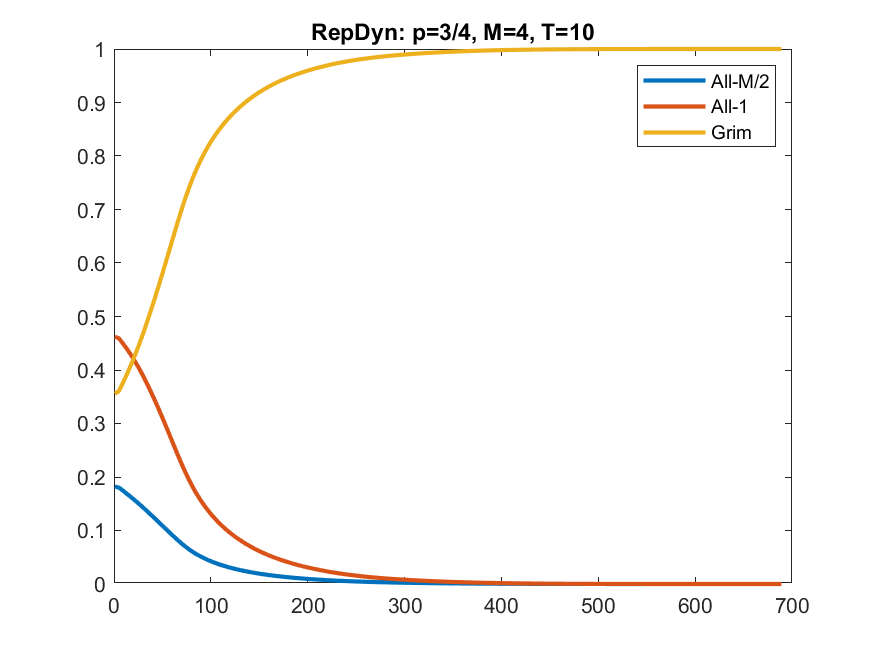
\includegraphics[width=\textwidth]{figures1/rep_timeseries_p075}
    \caption{$p = 3/4$}
  \end{subfigure}
  \hfill
  \begin{subfigure}[b]{0.48\textwidth}
    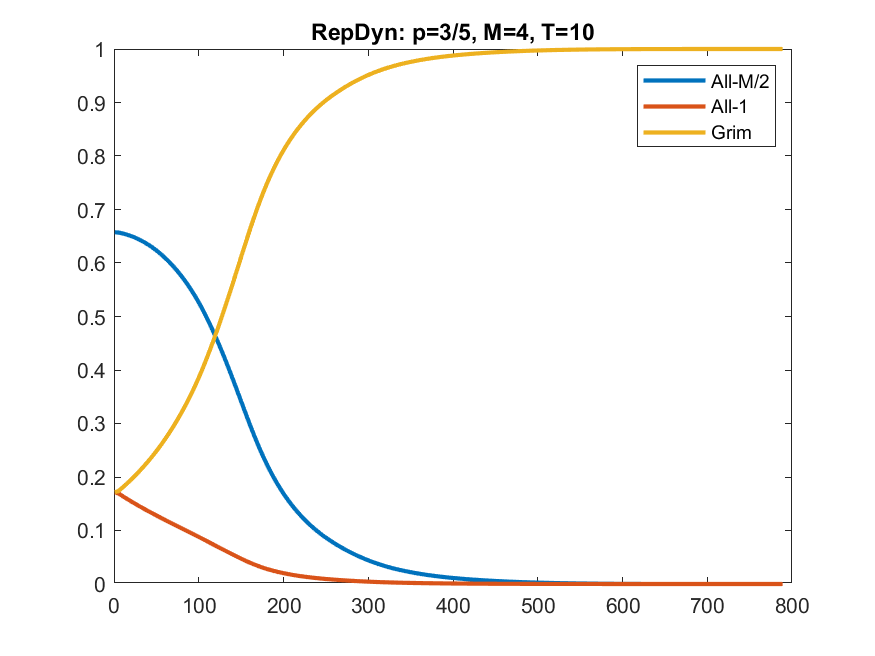
\includegraphics[width=\textwidth]{figures1/rep_timeseries_p060}
    \caption{$p = 3/5$}
  \end{subfigure}
  \caption{Replicator dynamics time series, Variation~1 ($M=4$, $T=10$).}
  \label{fig:v1_rep_timeseries}
\end{figure}

\subsubsection*{Parameter Sensitivity}

\begin{figure}[H]
  \centering
  \includegraphics[width=\textwidth]{figures1/rep_overlay_vary_p}
  \caption{Replicator dynamics: effect of varying $p \in \{3/5,\,2/3,\,3/4,\,9/10\}$
           ($M=4$, $T=10$), Variation~1.}
  \label{fig:v1_rep_vary_p}
\end{figure}

\begin{figure}[H]
  \centering
  \includegraphics[width=\textwidth]{figures1/rep_overlay_vary_M}
  \caption{Replicator dynamics: effect of varying $M \in \{2,4,6,8\}$
           ($p=3/4$, $T=10$), Variation~1.}
  \label{fig:v1_rep_vary_M}
\end{figure}

\begin{figure}[H]
  \centering
  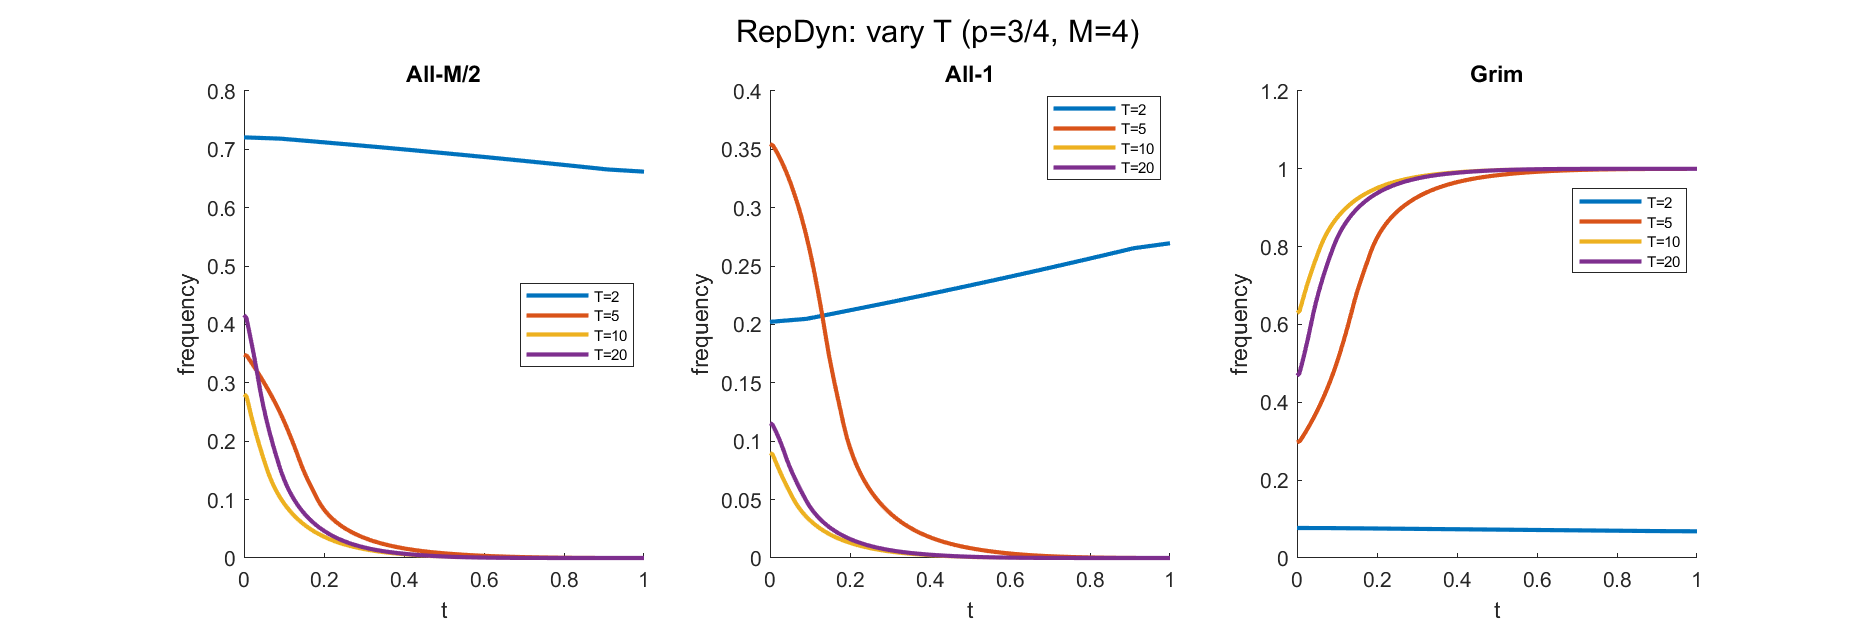
\includegraphics[width=\textwidth]{figures1/rep_overlay_vary_T}
  \caption{Replicator dynamics: effect of varying $T \in \{2,5,10,20\}$
           ($p=3/4$, $M=4$), Variation~1.}
  \label{fig:v1_rep_vary_T}
\end{figure}

\begin{figure}[H]
  \centering
  \includegraphics[width=\textwidth]{figures1/rep_overlay_vary_x0_p075}
  \caption{Replicator dynamics: effect of varying initial condition $x_0$
           ($p=3/4$, $M=4$, $T=10$), Variation~1.}
  \label{fig:v1_rep_x0_p075}
\end{figure}

\begin{figure}[H]
  \centering
  \includegraphics[width=\textwidth]{figures1/rep_overlay_vary_x0_p060}
  \caption{Replicator dynamics: effect of varying initial condition $x_0$
           ($p=3/5$, $M=4$, $T=10$), Variation~1.}
  \label{fig:v1_rep_x0_p060}
\end{figure}

\subsection{Markov Chain Dynamics}

The population state is $s = (s_1, s_2, s_3)$ with $s_1+s_2+s_3 = N$ and
$s_i \geq 0$ integers. The per-player payoff of strategy $m$ in state $s$ is:
\[
  q_m(s) = (s_m - 1)\,C(m,m) + \sum_{n \neq m} s_n\,C(m,n).
\]

Under the \textbf{Pairwise Proportional Imitation (PPI)} revision protocol, a
randomly selected player using strategy $m_1$ switches to $m_2$ with probability:
\[
  \varrho_{m_1 m_2}(s) =
  \frac{x_{m_2}\,[q_{m_2}(s) - q_{m_1}(s)]_+}
       {\sum_m x_m\,[q_m(s) - q_{m_1}(s)]_+}.
\]

\noindent\textbf{Absorbing states.} Because $C(1,1) = T \cdot (M/2) = 20
\neq 40 = C(3,3)$, Grim earns strictly more than All-$M/2$ on the $s_2=0$
face. The \textbf{only absorbing states} are the three pure vertices:
$(N,0,0)$, $(0,N,0)$, $(0,0,N)$.

\begin{figure}[H]
  \centering
  \begin{subfigure}[b]{0.48\textwidth}
    \includegraphics[width=\textwidth]{figures1/mark_stategraph_p075}
    \caption{$p = 3/4$}
    \label{fig:v1_stategraph_p075}
  \end{subfigure}
  \hfill
  \begin{subfigure}[b]{0.48\textwidth}
    \includegraphics[width=\textwidth]{figures1/mark_stategraph_p060}
    \caption{$p = 3/5$}
    \label{fig:v1_stategraph_p060}
  \end{subfigure}
  \caption{Markov state transition graphs, Variation~1 ($M=4$, $T=10$, $N=10$).
           Blue dots: absorbing (pure) states. Red dots: transient states.
           Arrow thickness indicates transition probability.}
  \label{fig:v1_stategraph_both}
\end{figure}

\begin{figure}[H]
  \centering
  \begin{subfigure}[b]{0.48\textwidth}
    \includegraphics[width=\textwidth]{figures1/mark_timeseries_p075}
    \caption{$p = 3/4$}
  \end{subfigure}
  \hfill
  \begin{subfigure}[b]{0.48\textwidth}
    \includegraphics[width=\textwidth]{figures1/mark_timeseries_p060}
    \caption{$p = 3/5$}
  \end{subfigure}
  \caption{Markov dynamics time series, Variation~1 ($M=4$, $T=10$, $N=10$, $T_m=100$,
           $s_0=[3,4,3]$).}
  \label{fig:v1_mark_timeseries}
\end{figure}

\subsubsection*{Parameter Sensitivity}

\begin{figure}[H]
  \centering
  \includegraphics[width=\textwidth]{figures1/mark_overlay_vary_p}
  \caption{Markov dynamics: effect of varying $p \in \{3/5,\,2/3,\,3/4,\,9/10\}$
           ($M=4$, $T=10$, $N=10$), Variation~1.}
  \label{fig:v1_mark_vary_p}
\end{figure}

\begin{figure}[H]
  \centering
  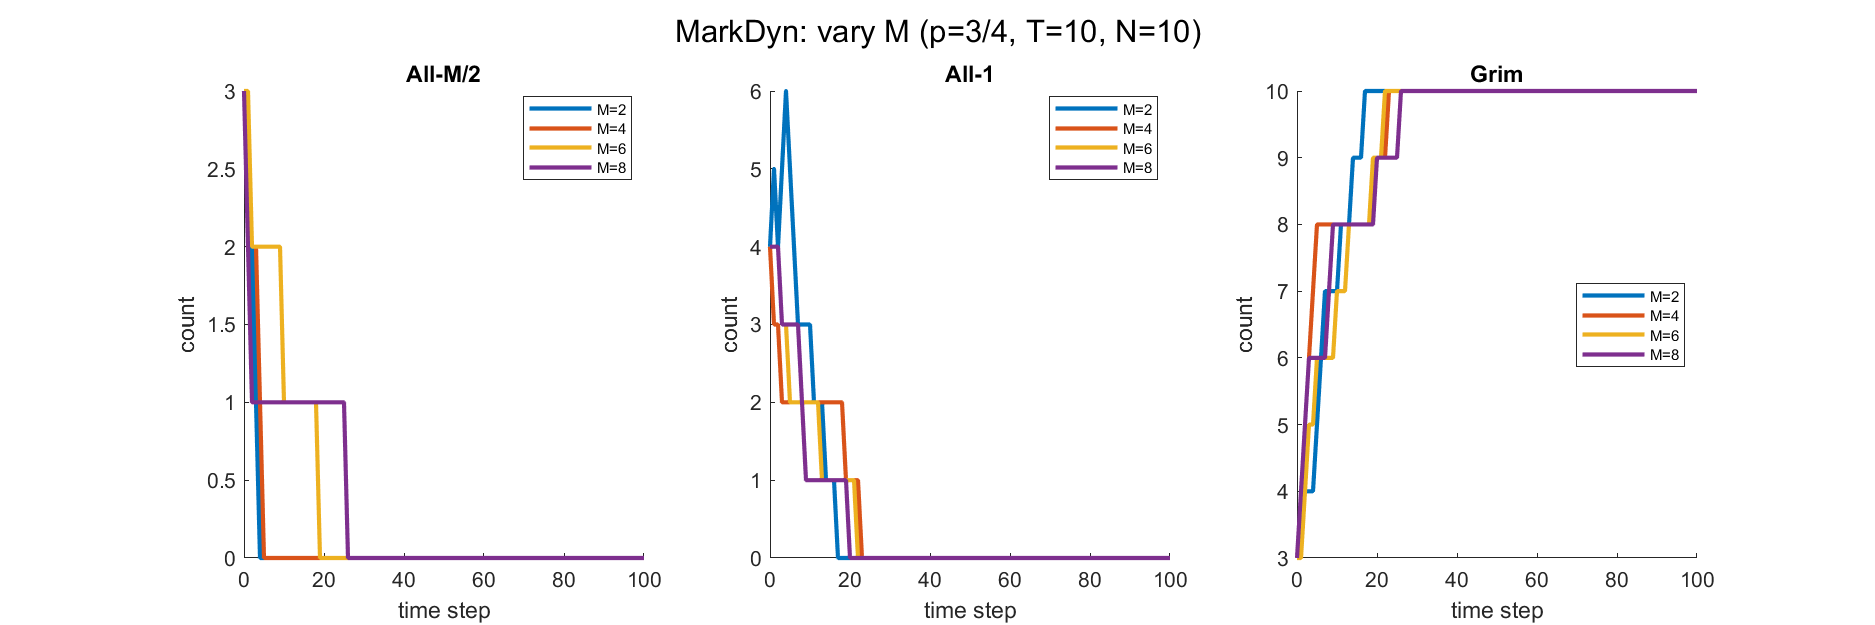
\includegraphics[width=\textwidth]{figures1/mark_overlay_vary_M}
  \caption{Markov dynamics: effect of varying $M \in \{2,4,6,8\}$
           ($p=3/4$, $T=10$, $N=10$), Variation~1.}
  \label{fig:v1_mark_vary_M}
\end{figure}

\begin{figure}[H]
  \centering
  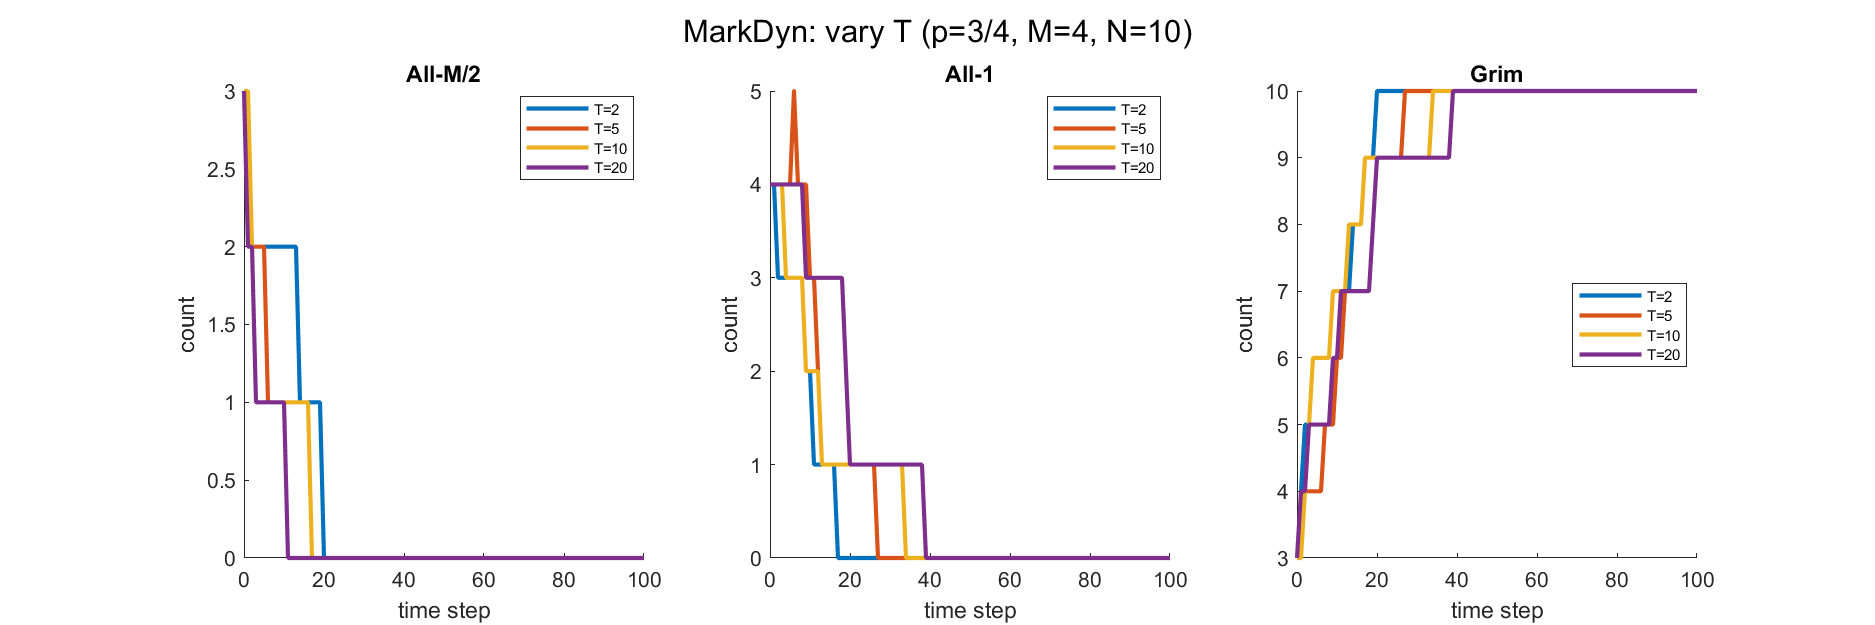
\includegraphics[width=\textwidth]{figures1/mark_overlay_vary_T}
  \caption{Markov dynamics: effect of varying $T \in \{2,5,10,20\}$
           ($p=3/4$, $M=4$, $N=10$), Variation~1.}
  \label{fig:v1_mark_vary_T}
\end{figure}

\begin{figure}[H]
  \centering
  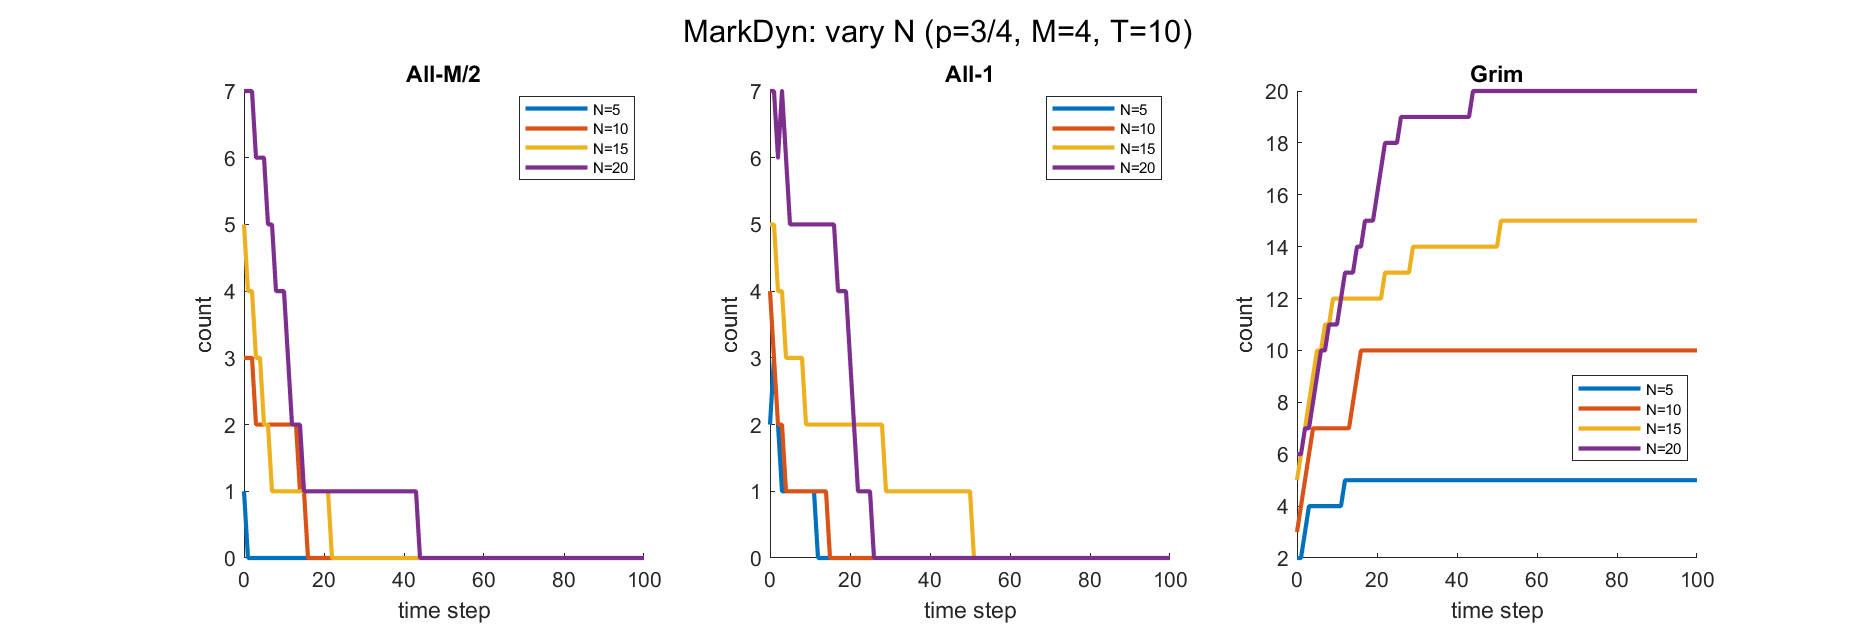
\includegraphics[width=\textwidth]{figures1/mark_overlay_vary_N}
  \caption{Markov dynamics: effect of varying $N \in \{5,10,15,20\}$
           ($p=3/4$, $M=4$, $T=10$), Variation~1.}
  \label{fig:v1_mark_vary_N}
\end{figure}

\begin{figure}[H]
  \centering
  \includegraphics[width=\textwidth]{figures1/mark_overlay_vary_s0_p075}
  \caption{Markov dynamics: effect of varying initial state $s_0$
           ($p=3/4$, $M=4$, $T=10$, $N=10$), Variation~1.}
  \label{fig:v1_mark_s0_p075}
\end{figure}

\begin{figure}[H]
  \centering
  \includegraphics[width=\textwidth]{figures1/mark_overlay_vary_s0_p060}
  \caption{Markov dynamics: effect of varying initial state $s_0$
           ($p=3/5$, $M=4$, $T=10$, $N=10$), Variation~1.}
  \label{fig:v1_mark_s0_p060}
\end{figure}

\subsection{Key Findings of Variation 1}

\begin{table}[H]
\centering
\caption{Comparison: original paper (All-$M$) vs.\ Variation~1 (All-$M/2$).}
\label{tab:v1_differences}
\small
\begin{tabular}{lll}
\toprule
Aspect & Original (All-$M$) & Variation~1 (All-$M/2$) \\
\midrule
Cooperator strategy       & Always play $\rho_M$       & Always play $\rho_{M/2}$ \\
$C(1,1)$                  & $T \cdot M = 40$           & $T \cdot (M/2) = 20$ \\
$C(3,3)$                  & $T \cdot M = 40$           & $T \cdot M = 40$ (unchanged) \\
Grim trigger vs cooperator & Never ($M \not< M$)        & Always ($M/2 < M$) \\
$s_2{=}0$ face absorbing? & Yes (entire face)          & No (only pure vertices) \\
Absorbing states          & $(0,N,0)$ + $s_2{=}0$ face & $(N,0,0)$, $(0,N,0)$, $(0,0,N)$ \\
\bottomrule
\end{tabular}
\end{table}

A critical threshold emerges at $p = 2/3$:
\begin{itemize}
  \item $p > 2/3$ (e.g.\ $p = 3/4$): the pure-defector state $(0,1,0)$ is
        asymptotically stable. Both Grim and All-$1$ can be long-run outcomes.
  \item $p < 2/3$ (e.g.\ $p = 3/5$): $(0,1,0)$ is unstable. All-$1$ is
        driven out; the population converges to the All-$M/2$--Grim edge.
\end{itemize}

%============================================================
\section{Variation 2: All-\texorpdfstring{$M/2$}{M/2}, All-1, and Grim ---\\
Rigorous Mathematical Analysis}
\label{sec:var2}
%============================================================

\subsection{Overview}

This variation provides a complete rigorous mathematical treatment of the same
three-strategy ISC game as Variation~1, deriving all Nash equilibria, stability
conditions of rest points, and evolutionarily stable strategies with full proofs.
The strategy set and payoff matrix $C$ are identical to Variation~1 (see
Tables~\ref{tab:v1_C_p075}--\ref{tab:v1_C_p060}); the large-$T$ approximation
is:
\begin{equation}\label{eq:v2_Capprox}
C \approx T\begin{bmatrix}
k & 3(1-p) & 3(1-p) \\
3p & 1 & 1 \\
3p & 1 & M
\end{bmatrix}, \quad k = M/2.
\end{equation}

\begin{figure}[H]
  \centering
  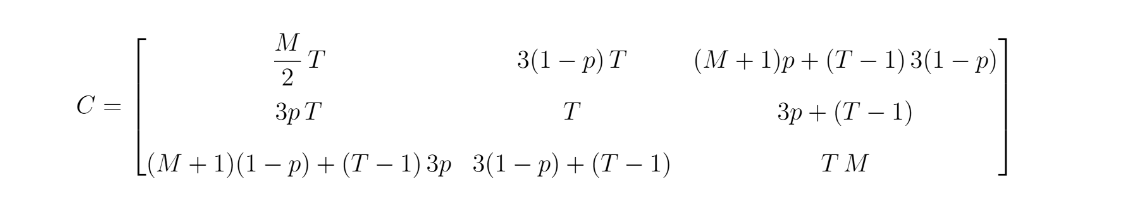
\includegraphics[width=0.9\textwidth]{figures2/c_matrix_figure}
  \caption{Symbolic payoff matrix $C$ for Variation~2.}
  \label{fig:v2_c_matrix}
\end{figure}

\subsection{Nash Equilibria}

\begin{definition}[Nash Equilibrium]
A pair of mixed strategies $(\hat\sigma_1,\hat\sigma_2)$ is a \emph{Nash
equilibrium} (NE) iff
\[
  \forall\sigma_1:\; Q_1(\hat\sigma_1,\hat\sigma_2)\geq Q_1(\sigma_1,\hat\sigma_2)
  \quad\text{and}\quad
  \forall\sigma_2:\; Q_2(\hat\sigma_1,\hat\sigma_2)\geq Q_2(\hat\sigma_1,\sigma_2).
\]
\end{definition}

\begin{proposition}[Pure-Strategy NE]\label{prop:v2_pure_NE}
For $M\geq 4$, $k=M/2$, and $T$ large enough:
\begin{enumerate}
  \item $\bigl((0,0,1),(0,0,1)\bigr)$ is a NE for all $p\in(\tfrac{1}{2},1]$.
  \item $\bigl((0,1,0),(0,1,0)\bigr)$ is a NE if and only if $p\geq\tfrac{2}{3}$.
  \item $\bigl((1,0,0),(1,0,0)\bigr)$ is a NE if and only if $p\leq \tfrac{k}{3}=\tfrac{M}{6}$.
\end{enumerate}
\end{proposition}

\begin{proof}
\textit{(1) Pure Grim.} For a deviation $(a,b,1-a-b)$:
$\delta Q_1 = a(TM-C(1,3))+b(TM-C(2,3)) \geq 0$, since $TM-C(1,3)\approx T(M-3+3p)>0$
and $TM-C(2,3)\approx T(M-1)>0$ for $M\geq 2$.

\textit{(2) Pure All-$1$.} Deviation toward strategy 1: $\delta Q_1 = aT(3p-2)$.
Deviation toward strategy 3: $\delta Q_1 = c(2-3p)$.
Both are non-negative iff $p\geq 2/3$.

\textit{(3) Pure All-$k$.} Deviation toward strategies 2 or 3:
$\delta Q_1 \approx T(k-3p)$, which is non-negative iff $p\leq k/3 = M/6$.
\end{proof}

\begin{remark}
For $M=4$ ($k=2$), the thresholds for parts (2) and (3) coincide at $p^*=2/3$:
\begin{itemize}
  \item $p<2/3$: $(0,0,1)$ and $(1,0,0)$ are pure NE; $(0,1,0)$ is not.
  \item $p>2/3$: $(0,0,1)$ and $(0,1,0)$ are pure NE; $(1,0,0)$ is not.
  \item $p=2/3$: only $(0,0,1)$ is a pure NE.
\end{itemize}
\end{remark}

\begin{proposition}[Mixed NE on the All-$k$/Grim Face]\label{prop:v2_mixed_13}
For $M\geq 4$ and large $T$, if $p < k/3 = M/6$, then
$\bigl((x_1^*,\,0,\,1-x_1^*),\;(x_1^*,\,0,\,1-x_1^*)\bigr)$
is a symmetric NE, where
\[
  x_1^* = \frac{2(M-3+3p)}{3(M-2)}.
\]
For $M=4$: $x_1^* = (1+3p)/3$. This rest point is \textbf{unstable}.
\end{proposition}

\begin{example}[NE for $M=4$, $T=10$]
For $p=3/4>2/3$: symmetric NE are $((0,0,1),(0,0,1))$ and $((0,1,0),(0,1,0))$;
no mixed NE exists.

For $p=3/5<2/3$: symmetric NE are $((0,0,1),(0,0,1))$, $((1,0,0),(1,0,0))$,
and $((x_1^*,0,1-x_1^*),(x_1^*,0,1-x_1^*))$ with $x_1^*=14/15\approx 0.933$.
\end{example}

\subsection{Replicator Dynamics and Stability}

The replicator equation is identical to Variation~1:
\[
  \dot{x}_m = x_m\left[(C{\bf x})_m - {\bf x}^\top C{\bf x}\right], \quad m=1,2,3.
\]

\begin{proposition}[Rest Points]\label{prop:v2_restpoints}
For $M=4$, $k=2$, and large $T$, the admissible rest points are:
\begin{enumerate}
  \item The three pure vertices $(1,0,0)$, $(0,1,0)$, $(0,0,1)$.
  \item The interior All-$k$/Grim rest point $(x_1^*,0,1-x_1^*)$ with $x_1^*=(1+3p)/3$,
        existing iff $p<2/3$.
\end{enumerate}
There are no interior rest points and no rest points on the All-$1$/Grim face.
\end{proposition}

\begin{proposition}[Stability of Pure Grim]\label{prop:v2_stab_grim}
For $M\geq 4$ and all $p\in(\tfrac{1}{2},1]$, the rest point $(0,0,1)$ is
asymptotically stable. The Jacobian eigenvalues are:
\[
  \lambda_1 = C(1,3)-C(3,3)\approx T(3-3p-M)<0, \quad
  \lambda_2 = C(2,3)-C(3,3)\approx T(1-M)<0.
\]
\end{proposition}

\begin{proposition}[Stability of Pure All-$1$]\label{prop:v2_stab_allone}
For $M\geq 4$ and large $T$:
\begin{enumerate}
  \item If $p>2/3$, then $(0,1,0)$ is asymptotically stable.
  \item If $p\leq 2/3$, then $(0,1,0)$ is unstable.
\end{enumerate}
The eigenvalues are $\lambda_1=T(2-3p)$ and $\lambda_3=2-3p$.
\end{proposition}

\begin{proposition}[Stability of Pure All-$k$]\label{prop:v2_stab_allk}
For $M=4$, $k=2$, and large $T$:
\begin{enumerate}
  \item If $p<2/3$, then $(1,0,0)$ is asymptotically stable.
  \item If $p\geq 2/3$, then $(1,0,0)$ is unstable.
\end{enumerate}
\end{proposition}

\begin{proposition}[Mixed All-$k$/Grim Rest Point is Unstable]
For $M=4$ and $p<2/3$, the rest point ${\bf x}^*=(x_1^*,0,1-x_1^*)$ is unstable.
On the All-$k$/Grim face: $\dot{x}_1=Tx_1(1-x_1)(3x_1-(1+3p))$, which is
negative for $x_1<x_1^*$ and positive for $x_1>x_1^*$: a repeller on this edge.
\end{proposition}

\subsubsection*{Phase Portraits and Sensitivity}

\begin{figure}[H]
  \centering
  \begin{subfigure}[b]{0.48\textwidth}
    \includegraphics[width=\textwidth]{figures2/rep_phase_p075}
    \caption{$p = 3/4$: $(0,1,0)$ and $(0,0,1)$ are stable.}
    \label{fig:v2_phase_p075}
  \end{subfigure}
  \hfill
  \begin{subfigure}[b]{0.48\textwidth}
    \includegraphics[width=\textwidth]{figures2/rep_phase_p060}
    \caption{$p = 3/5$: $(1,0,0)$ and $(0,0,1)$ are stable; mixed rest point at $x_1^*\approx0.933$.}
    \label{fig:v2_phase_p060}
  \end{subfigure}
  \caption{Phase portraits, Variation~2 ($M=4$, $T=10$).}
  \label{fig:v2_phase_both}
\end{figure}

\begin{figure}[H]
  \centering
  \includegraphics[width=\textwidth]{figures2/rep_overlay_vary_p}
  \caption{Replicator dynamics: effect of $p \in \{3/5,\,2/3,\,3/4,\,9/10\}$
           ($M=4$, $T=10$), Variation~2.}
  \label{fig:v2_rep_vary_p}
\end{figure}

\begin{figure}[H]
  \centering
  \includegraphics[width=\textwidth]{figures2/rep_overlay_vary_M}
  \caption{Replicator dynamics: effect of $M \in \{2,4,6,8\}$ ($p=3/4$, $T=10$),
           Variation~2. For larger $M$, the threshold $p^*=M/6$ shifts.}
  \label{fig:v2_rep_vary_M}
\end{figure}

\begin{figure}[H]
  \centering
  \includegraphics[width=\textwidth]{figures2/rep_overlay_vary_x0_p075}
  \caption{Replicator dynamics: initial condition sensitivity ($p=3/4$, $M=4$, $T=10$),
           Variation~2.}
  \label{fig:v2_rep_x0_p075}
\end{figure}

\begin{figure}[H]
  \centering
  \includegraphics[width=\textwidth]{figures2/rep_overlay_vary_x0_p060}
  \caption{Replicator dynamics: initial condition sensitivity ($p=3/5$, $M=4$, $T=10$),
           Variation~2.}
  \label{fig:v2_rep_x0_p060}
\end{figure}

\subsection{Evolutionarily Stable Strategies}

\begin{definition}[ESS]
A mixed strategy $\hat{\bf x}$ is an \emph{evolutionarily stable strategy}
(ESS) iff for all ${\bf x}\neq\hat{\bf x}$:
$\hat{\bf x}^\top C\hat{\bf x} \geq {\bf x}^\top C\hat{\bf x}$,
and equality implies $\hat{\bf x}^\top C{\bf x} > {\bf x}^\top C{\bf x}$.
\end{definition}

\begin{proposition}[Pure Grim is Always ESS]
For $M\geq 4$ and large $T$, $(0,0,1)$ is the unique ESS for all $p$. The
deviation gain $\hat{\bf x}^\top C\hat{\bf x}-{\bf x}^\top C\hat{\bf x}\approx
aT(M-3+3p)+bT(M-1)>0$ for all ${\bf x}\neq(0,0,1)$.
\end{proposition}

\begin{proposition}[Conditional ESS]
\begin{enumerate}
  \item $(0,1,0)$ is an ESS if and only if $p>2/3$.
  \item $(1,0,0)$ is an ESS if and only if $p<2/3$.
  \item The mixed rest point $(x_1^*,0,1-x_1^*)$ is never an ESS (it is unstable).
\end{enumerate}
\end{proposition}

\subsection{Markov Chain Analysis}

The Markov chain model and PPI protocol are as in Variation~1.

\begin{proposition}[Absorbing States and Interior Transitions]
For $M\geq 4$, $N\geq 4$, and large $T$, the only absorbing states are
$(N,0,0)$, $(0,N,0)$, $(0,0,N)$. In the interior, all transitions from
All-$1$ go south/southeast (toward Grim or All-$k$), never north. The
All-$k$--Grim direction is governed by:
\begin{itemize}
  \item $p>2/3$: west transitions (All-$k\to$Grim); the $s_2=0$ face is
        absorbed entirely into $(0,0,N)$.
  \item $p<2/3$: east transitions (Grim$\to$All-$k$); the $s_2=0$ face
        is separated by the line $\ell:\;s_1(2-3p)=s_3(1+3p)-2$.
\end{itemize}
\end{proposition}

\begin{figure}[H]
  \centering
  \begin{subfigure}[b]{0.48\textwidth}
    \includegraphics[width=\textwidth]{figures2/mark_stategraph_p075}
    \caption{$p = 3/4$}
    \label{fig:v2_stategraph_p075}
  \end{subfigure}
  \hfill
  \begin{subfigure}[b]{0.48\textwidth}
    \includegraphics[width=\textwidth]{figures2/mark_stategraph_p060}
    \caption{$p = 3/5$}
    \label{fig:v2_stategraph_p060}
  \end{subfigure}
  \caption{Markov state transition graphs, Variation~2 ($M=4$, $T=10$, $N=10$).}
  \label{fig:v2_stategraph_both}
\end{figure}

\begin{figure}[H]
  \centering
  \begin{subfigure}[b]{0.48\textwidth}
    \includegraphics[width=\textwidth]{figures2/mark_timeseries_p075}
    \caption{$p = 3/4$}
  \end{subfigure}
  \hfill
  \begin{subfigure}[b]{0.48\textwidth}
    \includegraphics[width=\textwidth]{figures2/mark_timeseries_p060}
    \caption{$p = 3/5$}
  \end{subfigure}
  \caption{Markov dynamics time series, Variation~2 ($M=4$, $T=10$, $N=10$, $s_0=[3,4,3]$).}
  \label{fig:v2_mark_timeseries}
\end{figure}

\begin{figure}[H]
  \centering
  \includegraphics[width=\textwidth]{figures2/mark_overlay_vary_p}
  \caption{Markov dynamics: effect of $p \in \{3/5,\,2/3,\,3/4,\,9/10\}$
           ($M=4$, $T=10$, $N=10$), Variation~2.}
  \label{fig:v2_mark_vary_p}
\end{figure}

\begin{figure}[H]
  \centering
  \includegraphics[width=\textwidth]{figures2/mark_overlay_vary_s0_p075}
  \caption{Markov dynamics: initial state sensitivity ($p=3/4$, $M=4$, $T=10$, $N=10$),
           Variation~2.}
  \label{fig:v2_mark_s0_p075}
\end{figure}

\begin{figure}[H]
  \centering
  \includegraphics[width=\textwidth]{figures2/mark_overlay_vary_s0_p060}
  \caption{Markov dynamics: initial state sensitivity ($p=3/5$, $M=4$, $T=10$, $N=10$),
           Variation~2.}
  \label{fig:v2_mark_s0_p060}
\end{figure}

\subsection{Connection to Learning Theory (Variations 1 \& 2)}

Both evolutionary game theory (EGT) and learning models describe adaptive
behaviour in strategic environments and generate identical dynamics under
distinct interpretations. In EGT, the population share $x_i(t)$ evolves via the
replicator dynamic. In learning models, individual agents adjust mixed strategies
based on reinforcement: the propensity $q_i$ to play action $i$ evolves as
$q_i(t+1) = q_i(t)+\alpha\pi_i(t)$, with $x_i(t)=q_i(t)/\sum_j q_j(t)$.
It can be shown~\cite{BorgersSarin1997} that in large populations and continuous
time this rule converges to the replicator dynamic.

In the ISC context:
\begin{itemize}
  \item \textbf{Evolutionary:} The fraction of players using Grim grows when
        Grim earns above-average payoffs; the stable outcomes represent
        population-level selection pressures governed by $p^*=2/3$.
  \item \textbf{Learning:} Individual players accumulate experience and shift
        probability toward more profitable strategies; Grim's superior self-play
        payoff $C(3,3)=TM$ means rational learners reinforce cooperative
        reciprocal strategies over time.
\end{itemize}

%============================================================
\section{Variation 3: Five-Strategy Extension ---\\
All-\texorpdfstring{$M$}{M}, All-1, Grim, Grim-Patient, Grim-Forgiver}
\label{sec:var3}
%============================================================

\subsection{Overview and New Strategies}

This variation restores the original All-$M$ strategy and augments the strategy
set with two new Grim variants, for a total of five strategies:

\begin{definition}[Five ISC Strategies]\label{def:v3_strats}
\hfill
\begin{enumerate}
  \item $\sigma_1$ (\textbf{All-$M$}): play $\rho_M$ in every round.
  \item $\sigma_2$ (\textbf{All-$1$}): play $\rho_1$ in every round.
  \item $\sigma_3$ (\textbf{Grim}): play $\rho_M$ until the opponent plays
        $\rho_m$ with $m<M$; then switch permanently to $\rho_1$.
  \item $\sigma_4$ (\textbf{Grim-Patient}): play $\rho_M$ until the opponent
        plays $\rho_m$ with $m<M$ for \emph{two consecutive rounds}; then
        switch permanently to $\rho_1$.
  \item $\sigma_5$ (\textbf{Grim-Forgiver}): play $\rho_M$; when the opponent
        plays $\rho_m$ with $m<M$, switch to $\rho_1$ for \emph{exactly two
        rounds}, then return unconditionally to $\rho_M$ and repeat.
\end{enumerate}
\end{definition}

Strategies $\sigma_1$, $\sigma_3$, $\sigma_4$, $\sigma_5$ all play $\rho_M$
when the opponent plays $\rho_M$. Consequently, none of them ever triggers
against each other; they all cooperate at $\rho_M$ throughout any matchup among
themselves.

\subsection{The Five-Strategy Payoff Matrix}

Let $n_3(T) = \lceil T/3 \rceil$.

\begin{proposition}[ISC Payoff Matrix]\label{prop:v3_Cmatrix}
\begin{equation}\label{eq:v3_C}
C = \begin{pmatrix}
T M & 3(1-p)T & TM & TM & TM \\[4pt]
3pT & T & 3p + (T-1) & 6p + (T-2) & 3p\,n_3 + (T-n_3) \\[4pt]
TM & 3(1-p)+(T-1) & TM & TM & TM \\[4pt]
TM & 6(1-p)+(T-2) & TM & TM & TM \\[4pt]
TM & 3(1-p)\,n_3+(T-n_3) & TM & TM & TM
\end{pmatrix}.
\end{equation}
\end{proposition}

\begin{proof}[Derivation sketch]
All matchups among $\{1,3,4,5\}$ yield $TM$ since no trigger is ever fired.
Against All-$1$: Grim plays $\rho_M$ in round 1 then triggers ($C(3,2)=3(1-p)+(T-1)$);
Grim-Patient plays $\rho_M$ in rounds 1--2 then triggers ($C(4,2)=6(1-p)+(T-2)$);
Grim-Forgiver cycles with period 3 ($C(5,2)=3(1-p)n_3+(T-n_3)$). All-$1$ earns
$3p$ per round against Grim's $\rho_M$ rounds, etc.
\end{proof}

\begin{remark}[Payoff degeneracy]
The matrix $C$ is highly degenerate: $C(i,j)=TM$ for all $i,j\in\{1,3,4,5\}$.
This means all four cooperating strategies earn identical payoffs against each other.
Moreover, $C(2,1)<C(2,3)<C(2,4)<C(2,5)$ always: Grim-Forgiver is the most
exploitable by All-$1$ because it repeatedly returns to full cooperation.
Conversely, $C(1,2)>C(3,2)>C(4,2)>C(5,2)$ for $p>2/3$.
\end{remark}

\begin{table}[H]
\centering
\caption{Payoff matrix $C$ for $p=3/4$, $M=4$, $T=10$, Variation~3.}
\label{tab:v3_C_p075}
\renewcommand{\arraystretch}{1.25}
\begin{tabular}{lccccc}
\toprule
          & All-$M$ & All-$1$ & Grim   & GrimP  & GrimF  \\
\midrule
All-$M$   & 40      & 7.5     & 40     & 40     & 40     \\
All-$1$   & 22.5    & 10      & 11.25  & 12.5   & 15     \\
Grim      & 40      & 9.75    & 40     & 40     & 40     \\
GrimP     & 40      & 9.5     & 40     & 40     & 40     \\
GrimF     & 40      & 9       & 40     & 40     & 40     \\
\bottomrule
\end{tabular}
\end{table}

\begin{table}[H]
\centering
\caption{Payoff matrix $C$ for $p=3/5$, $M=4$, $T=10$, Variation~3.}
\label{tab:v3_C_p060}
\renewcommand{\arraystretch}{1.25}
\begin{tabular}{lccccc}
\toprule
          & All-$M$ & All-$1$ & Grim   & GrimP  & GrimF  \\
\midrule
All-$M$   & 40      & 12      & 40     & 40     & 40     \\
All-$1$   & 18      & 10      & 10.8   & 11.6   & 13.4   \\
Grim      & 40      & 10.2    & 40     & 40     & 40     \\
GrimP     & 40      & 10.4    & 40     & 40     & 40     \\
GrimF     & 40      & 11      & 40     & 40     & 40     \\
\bottomrule
\end{tabular}
\end{table}

\subsection{Nash Equilibria}

\begin{proposition}[Pure-Strategy NE]\label{prop:v3_pureNE}
For $M\geq 4$ and large $T$:
\begin{enumerate}
  \item All pure states $(\sigma_i,\sigma_i)$ for $i\in\{1,3,4,5\}$ are NE.
  \item $(\sigma_2,\sigma_2)$ is a NE if and only if $p\geq\tfrac{2}{3}$.
\end{enumerate}
\end{proposition}

\begin{proposition}[Cooperative Equilibrium Set]\label{prop:v3_coopset}
For every $M\geq 4$ and large $T$, all mixed strategies of the form
$\mathbf{x}=(x_1,0,x_3,x_4,x_5)$ with $x_1+x_3+x_4+x_5=1$ are Nash equilibria.
The ISC has a \emph{continuum} of NE due to the payoff degeneracy $C(i,j)=TM$
for all $i,j\in\{1,3,4,5\}$.
\end{proposition}

\subsection{Replicator Dynamics}

Let $\mathbf{x}=(x_1,x_2,x_3,x_4,x_5)$ with $\sum_m x_m=1$. The replicator equation is:
\[
  \dot{x}_m = x_m\Bigl[(C\mathbf{x})_m - \mathbf{x}^\top C\mathbf{x}\Bigr],
  \quad m=1,\ldots,5.
\]

\begin{proposition}[Rest Points]
The admissible rest points are:
\begin{enumerate}
  \item The entire cooperative face $\mathcal{F} = \{\mathbf{x}\in S_5 : x_2=0\}$.
  \item The pure All-$1$ state $(0,1,0,0,0)$.
  \item For $p\geq\tfrac{2}{3}$, all mixtures between All-$1$ and any
        cooperating profile.
\end{enumerate}
Within $\mathcal{F}$, the replicator dynamics has \emph{no drift} --- there is
no selection pressure among cooperating strategies.
\end{proposition}

\begin{proposition}[Stability of $\mathcal{F}$]
For $M\geq 4$ and large $T$:
\begin{enumerate}
  \item If $p<\tfrac{2}{3}$: $\mathcal{F}$ is asymptotically stable
        (All-$1$ cannot invade).
  \item If $p>\tfrac{2}{3}$: $\mathcal{F}$ is unstable (All-$1$ invades).
  \item If $p=\tfrac{2}{3}$: $\mathcal{F}$ is unstable (Grim variants invade).
\end{enumerate}
The eigenvalue for All-$1$ invasion is $\mu_m = C(m,2) - T$, which is positive
(cooperative strategy invades All-$1$) iff $p<2/3$ for all $m\in\{1,3,4,5\}$.
\end{proposition}

\begin{proposition}[Grim Variant Ranking Under All-$1$ Invasion]
For $p>2/3$, when the population is near $\mathcal{F}$ with a small fraction
$\varepsilon$ of All-$1$ invaders, the fitness ranking is
$f_3>f_4>f_5>f_1$: Grim is most resistant to exploitation, and Grim-Forgiver
is least resistant (though more resistant than All-$M$).
\end{proposition}

\subsubsection*{Pentagon Phase Portrait}

Because $S_5$ is four-dimensional, we represent dynamics using a
\emph{pentagon projection}: each strategy $\sigma_m$ is placed at vertex $m$
of a regular pentagon, and a population state is projected to
$(X,Y)=\sum_m x_m(\cos\theta_m, \sin\theta_m)$ where $\theta_m = \pi/2 - 2\pi(m-1)/5$.

\begin{figure}[H]
  \centering
  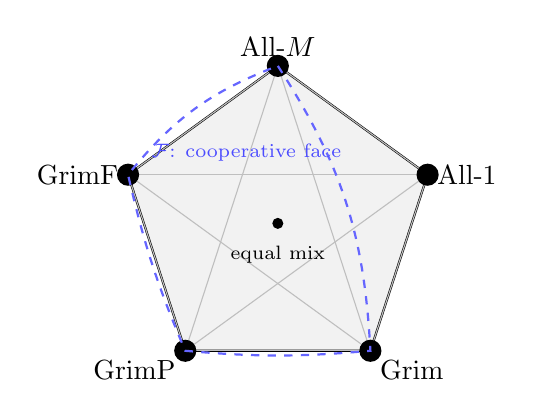
\begin{tikzpicture}[scale=2.0]
    \coordinate (v1) at ({cos(90)},{sin(90)});
    \coordinate (v2) at ({cos(90-72)},{sin(90-72)});
    \coordinate (v3) at ({cos(90-144)},{sin(90-144)});
    \coordinate (v4) at ({cos(90-216)},{sin(90-216)});
    \coordinate (v5) at ({cos(90-288)},{sin(90-288)});
    \fill[gray!10] (v1)--(v2)--(v3)--(v4)--(v5)--cycle;
    \draw[thick] (v1)--(v2)--(v3)--(v4)--(v5)--cycle;
    \foreach \i in {1,...,5} {
      \foreach \j in {1,...,5} {
        \ifnum\i<\j
          \draw[gray!50,thin] (v\i)--(v\j);
        \fi
      }
    }
    \foreach \i in {1,...,5} { \fill (v\i) circle (2pt); }
    \node[above] at (v1) {All-$M$};
    \node[right] at (v2) {All-$1$};
    \node[below right] at (v3) {Grim};
    \node[below left] at (v4) {GrimP};
    \node[left] at (v5) {GrimF};
    \fill (0,0) circle (1pt);
    \node[below, font=\scriptsize] at (0,-0.08) {equal mix};
    \draw[blue!60, thick, dashed] (v1) to[bend left=15] (v3) to[bend left=5] (v4)
      to[bend left=5] (v5) to[bend left=15] (v1);
    \node[blue!70, font=\scriptsize] at (-0.2,0.45) {$\mathcal{F}$: cooperative face};
  \end{tikzpicture}
  \caption{Pentagon representation of the five-strategy simplex $S_5$.
           The dashed region $\mathcal{F}$ is the cooperative face; all points
           in $\mathcal{F}$ are rest points of the replicator dynamics.}
  \label{fig:v3_pentagon}
\end{figure}

\begin{figure}[H]
  \centering
  \begin{subfigure}[b]{0.48\textwidth}
    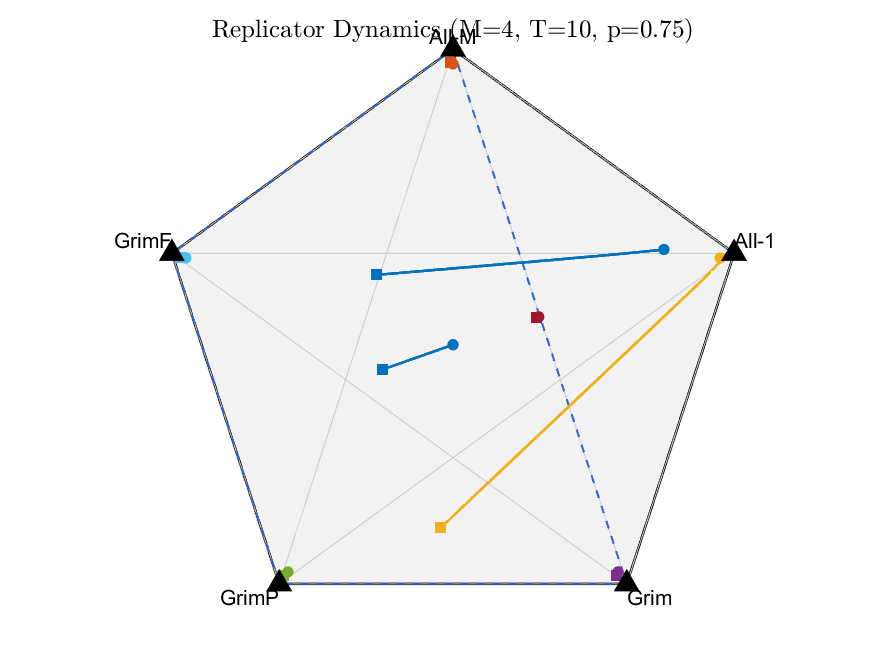
\includegraphics[width=\textwidth]{figures3/rep_phase_p075}
  \end{subfigure}
  \hfill
  \begin{subfigure}[b]{0.48\textwidth}
    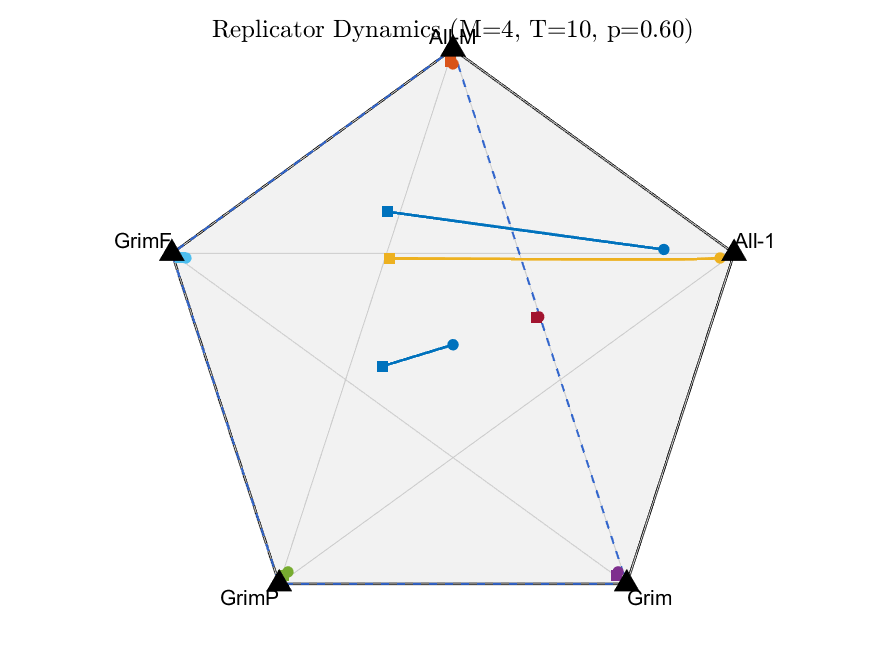
\includegraphics[width=\textwidth]{figures3/rep_phase_p060}
  \end{subfigure}
  \caption{Phase portraits on the pentagon, Variation~3 ($M=4$, $T=10$).}
  \label{fig:v3_phase_both}
\end{figure}

\begin{figure}[H]
  \centering
  \begin{subfigure}[b]{0.48\textwidth}
    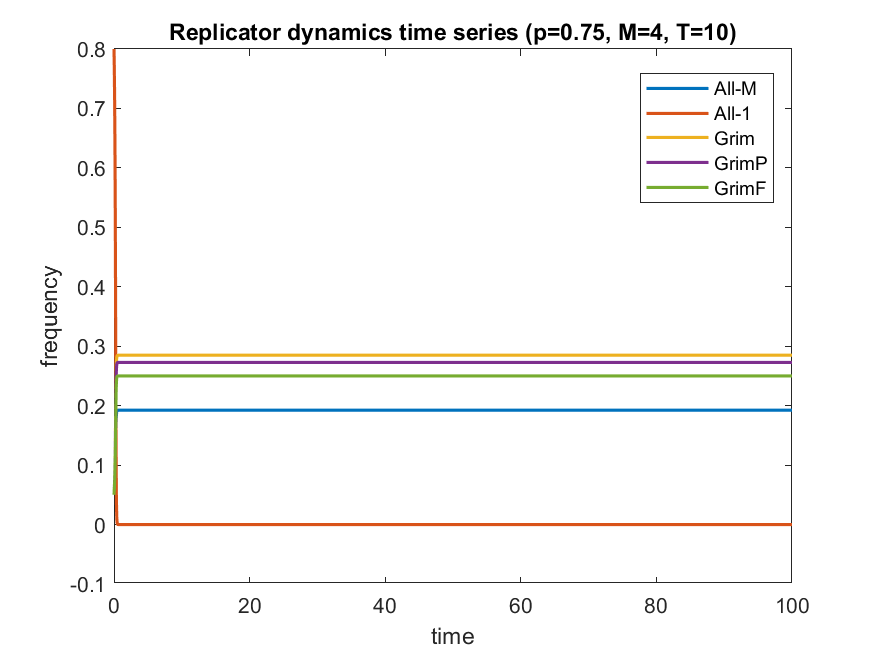
\includegraphics[width=\textwidth]{figures3/rep_timeseries_p075}
    \caption{$p=3/5$.}
  \end{subfigure}
  \caption{Replicator dynamics time series, Variation~3 ($M=4$, $T=10$).
           Line colours: All-$M$ blue, All-$1$ red, Grim green, GrimP orange, GrimF purple.}
  \label{fig:v3_rep_timeseries}
\end{figure}

\begin{figure}[H]
  \centering
  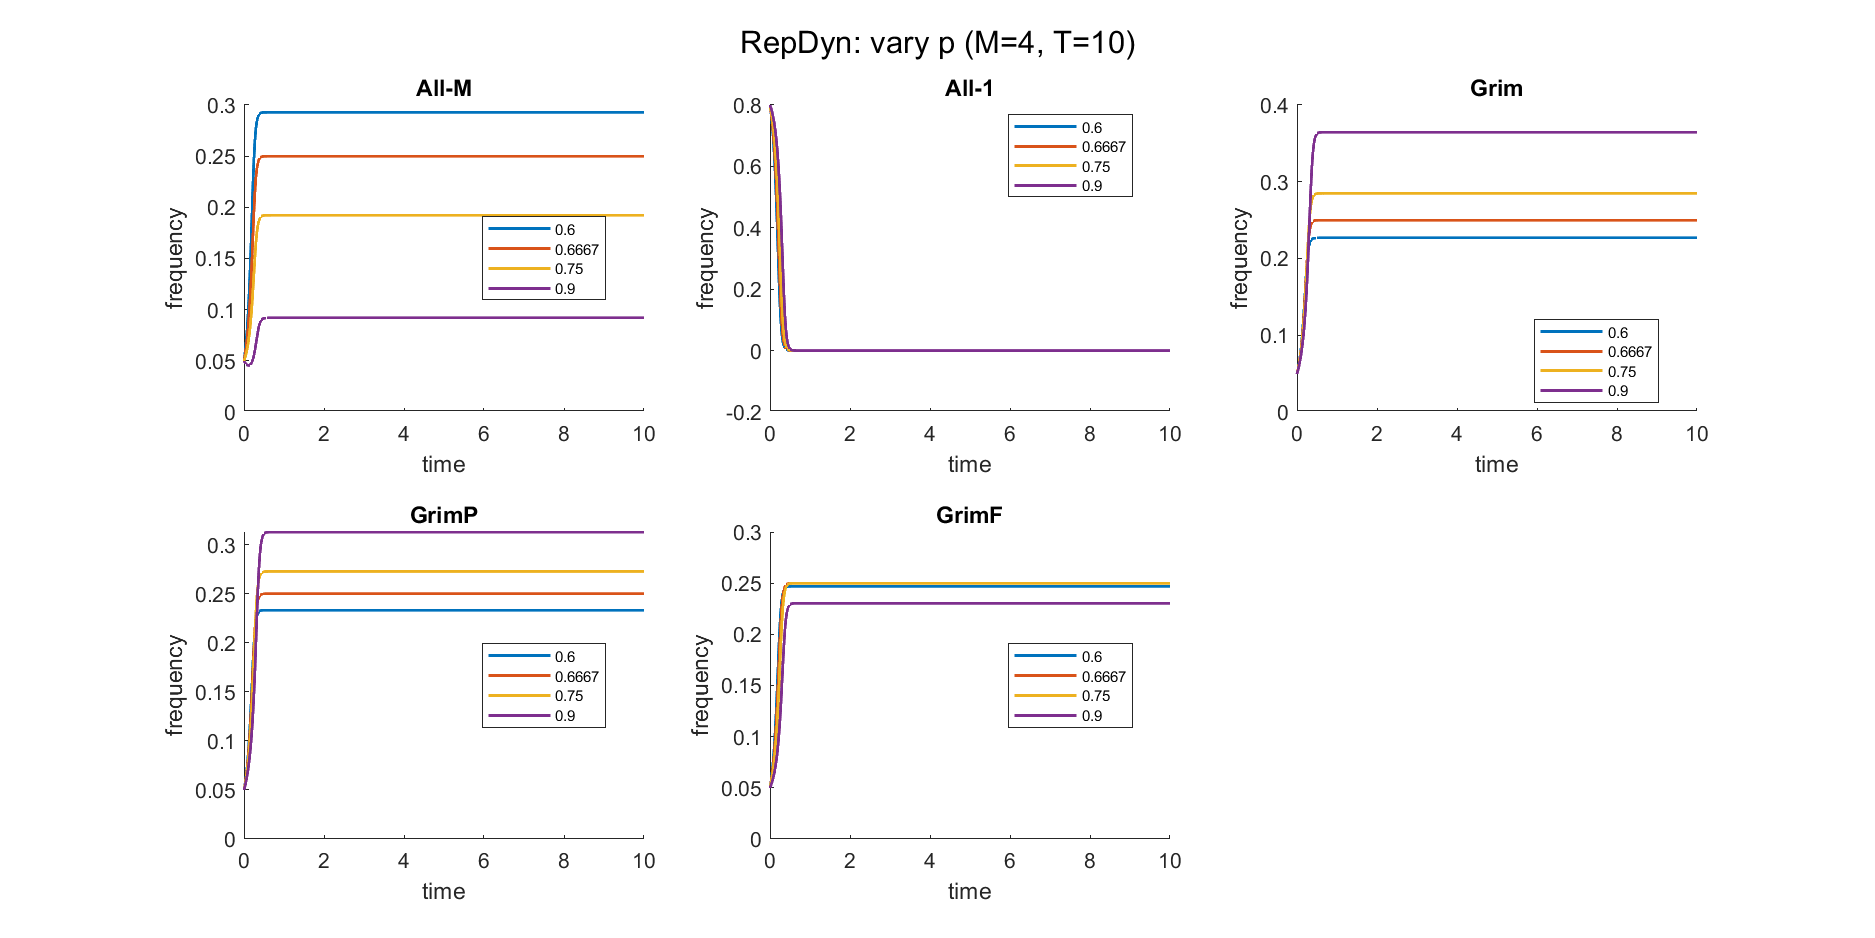
\includegraphics[width=\textwidth]{figures3/rep_overlay_vary_p}
  \label{fig:v3_rep_vary_p}
\end{figure}

\begin{figure}[H]
  \centering
  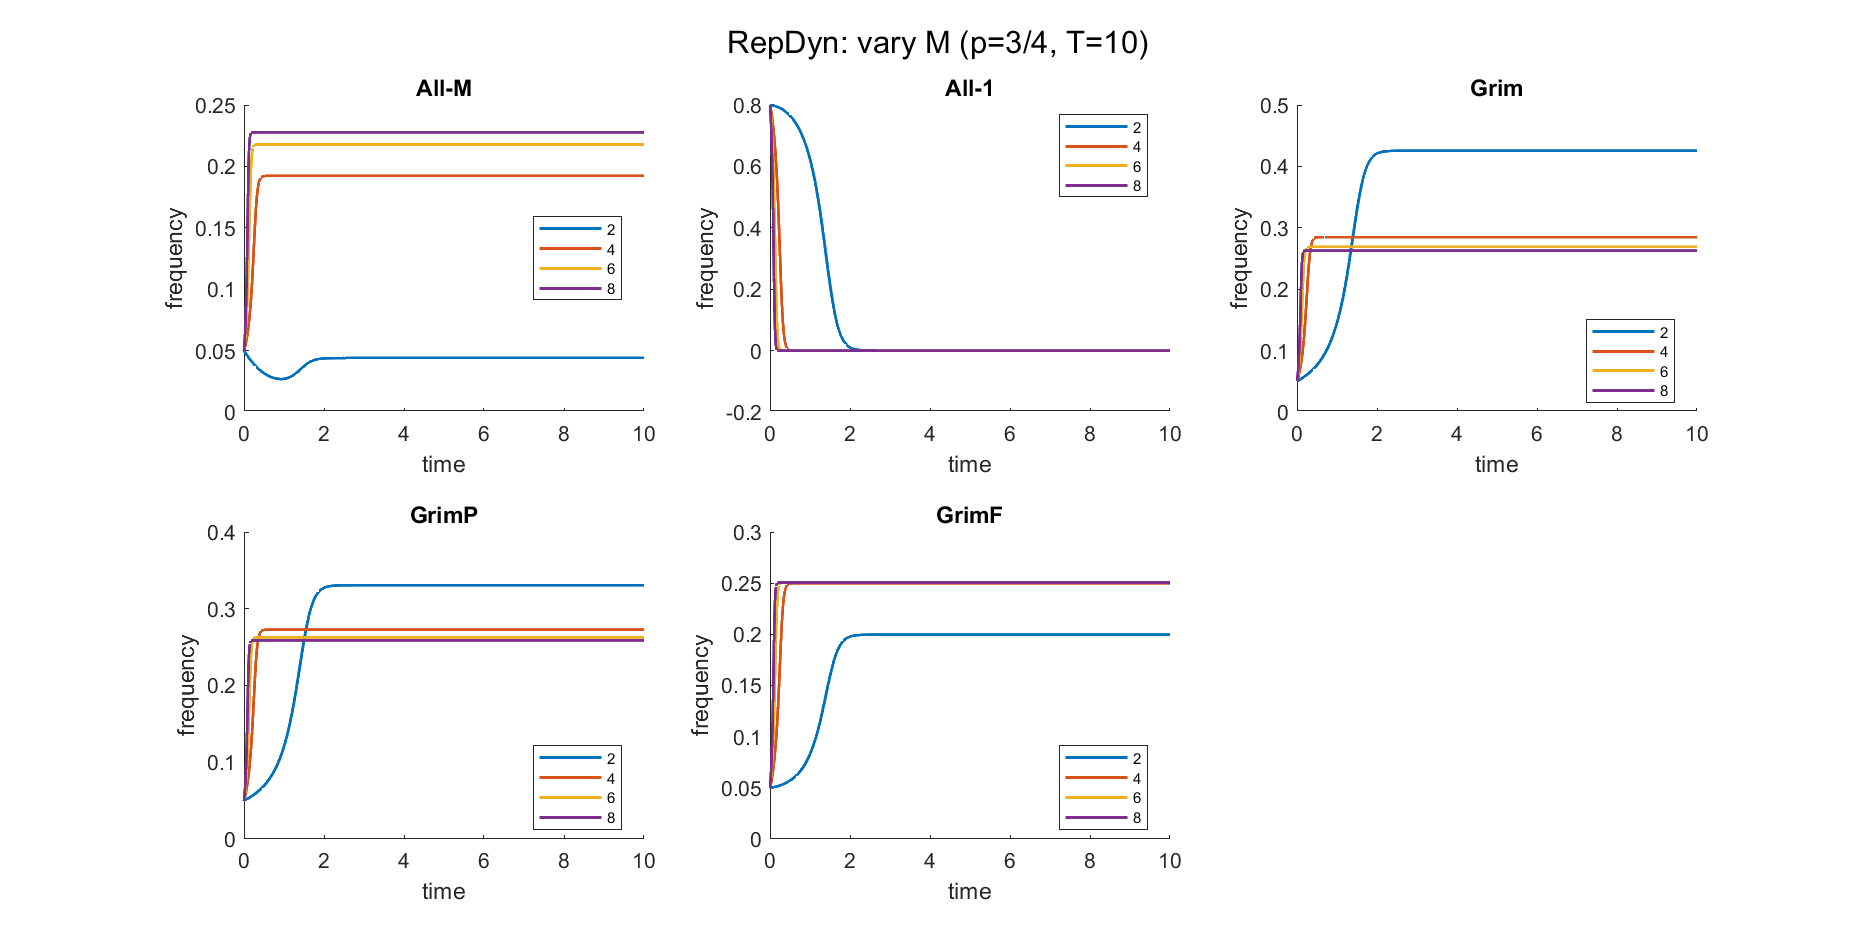
\includegraphics[width=\textwidth]{figures3/rep_overlay_vary_M}
  \label{fig:v3_rep_vary_M}
\end{figure}

\begin{figure}[H]
  \centering
  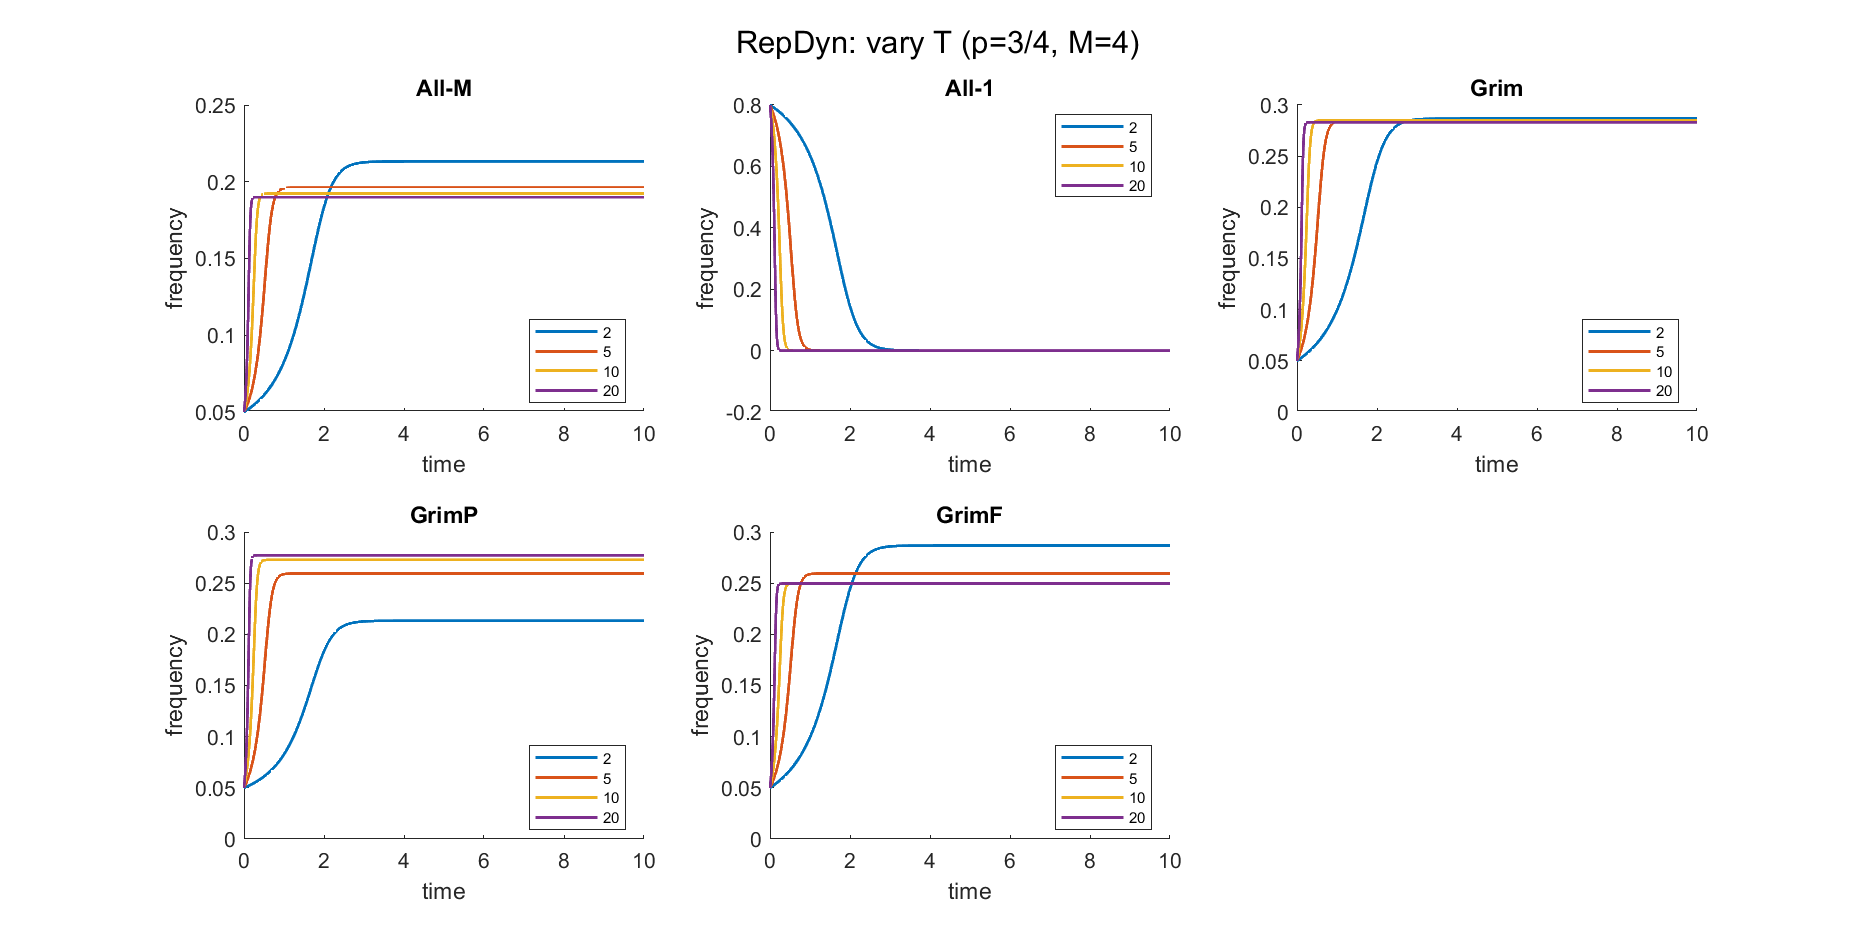
\includegraphics[width=\textwidth]{figures3/rep_overlay_vary_T}
  \label{fig:v3_rep_vary_T}
\end{figure}

\subsection{Evolutionary Stable Strategies}

\begin{proposition}[No Pure ESS from Cooperating Strategies]
For $M\geq 4$ and large $T$, no pure strategy $\sigma_i$ with $i\in\{1,3,4,5\}$
is an ESS, because any other cooperating strategy $\sigma_j$ ($j\neq i$, $j\in\{1,3,4,5\}$)
earns exactly the same payoff $TM$ as $\sigma_i$ against $\sigma_i$, violating
the strict ESS condition.
\end{proposition}

\begin{proposition}[All-$1$ ESS Condition]\label{prop:v3_ESSA1}
For $M\geq 4$ and large $T$:
\begin{enumerate}
  \item If $p>\tfrac{2}{3}$: $(0,1,0,0,0)$ is an ESS.
  \item If $p\leq\tfrac{2}{3}$: $(0,1,0,0,0)$ is not an ESS.
\end{enumerate}
\end{proposition}

\begin{proposition}[No Interior ESS]
No mixed strategy in the interior of $\mathcal{F}$ is an ESS, because points
in $\mathcal{F}$ are neutral to perturbations within $\mathcal{F}$.
\end{proposition}

\subsection{Markov Chain Analysis}

The population state is $\mathbf{s}=(s_1,s_2,s_3,s_4,s_5)$ with $\sum_m s_m=N$.

\begin{proposition}[Absorbing States]\label{prop:v3_absorbing}
For $M\geq 4$, $N\geq 2$, and large $T$, the absorbing states are:
\begin{enumerate}
  \item The pure All-$1$ state $(0,N,0,0,0)$.
  \item The entire cooperative face:
        $\mathcal{A} = \{(s_1,0,s_3,s_4,s_5) : s_1+s_3+s_4+s_5=N\}$.
\end{enumerate}
There are $\binom{N+3}{3}+1$ absorbing states in total.
\end{proposition}

This is a significant generalisation of the original paper: the entire $s_2=0$
four-dimensional face is absorbing, because all four cooperating strategies earn
identical payoffs $TM$ against each other.

\begin{figure}[H]
  \centering
  \begin{subfigure}[b]{0.48\textwidth}
    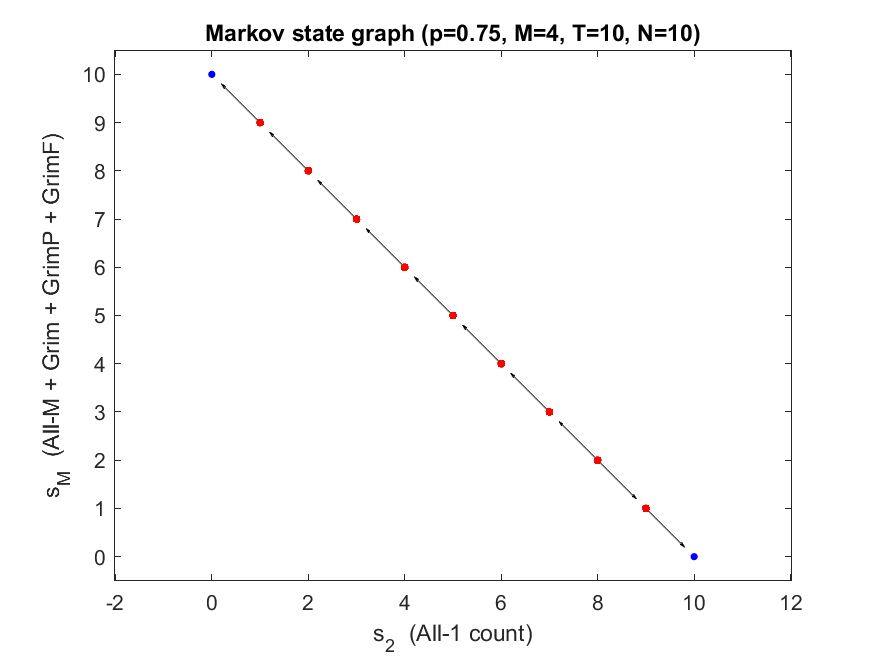
\includegraphics[width=\textwidth]{figures3/mark_stategraph_p075}
    \caption{$p=3/4$.}
  \end{subfigure}
  \hfill
  \begin{subfigure}[b]{0.48\textwidth}
    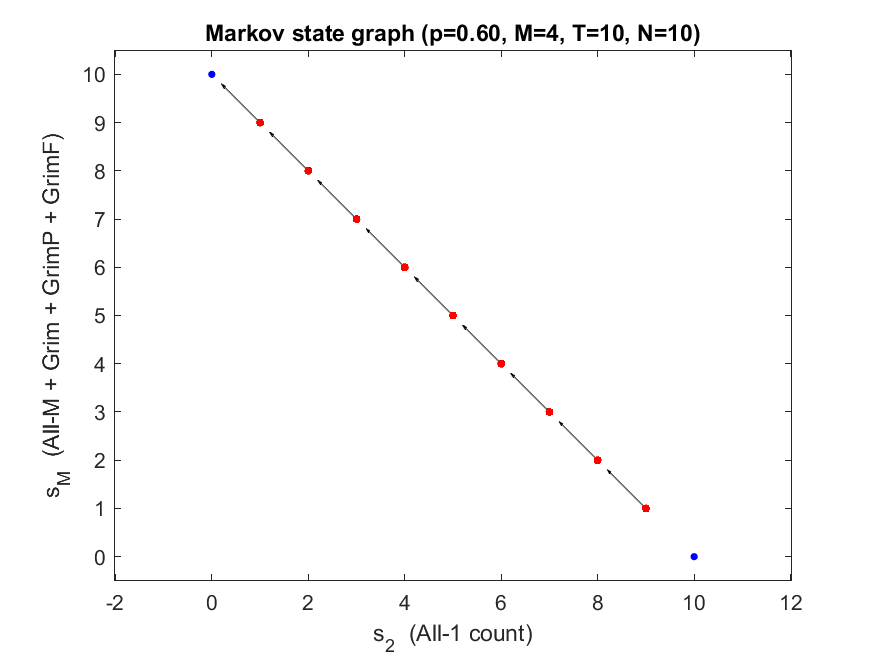
\includegraphics[width=\textwidth]{figures3/mark_stategraph_p060}
  \label{fig:v3_stategraph_both}
  \end{subfigure}
\end{figure}

\begin{figure}[H]
  \centering
  \begin{subfigure}[b]{0.48\textwidth}
    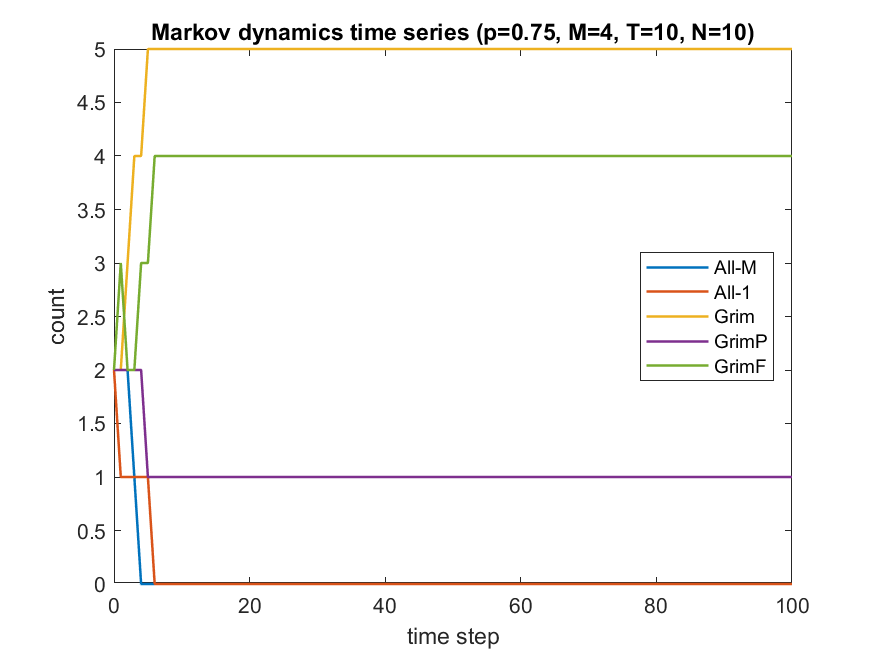
\includegraphics[width=\textwidth]{figures3/mark_timeseries_p075}
    \caption{$p=3/4$.}
  \end{subfigure}
  \hfill
  \begin{subfigure}[b]{0.48\textwidth}
    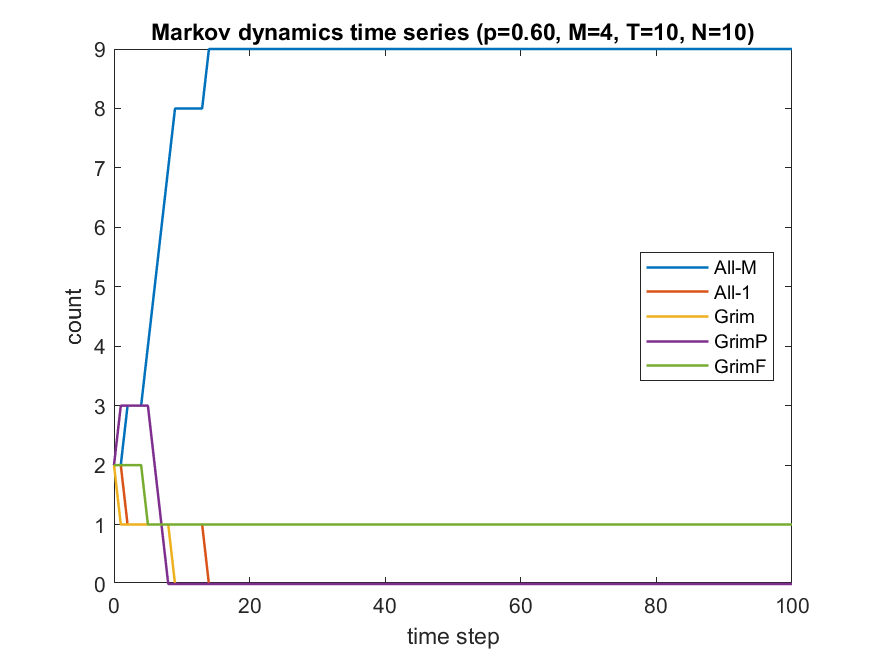
\includegraphics[width=\textwidth]{figures3/mark_timeseries_p060}
  \label{fig:v3_mark_timeseries}
  \end{subfigure}
\end{figure}

\begin{figure}[H]
  \centering
  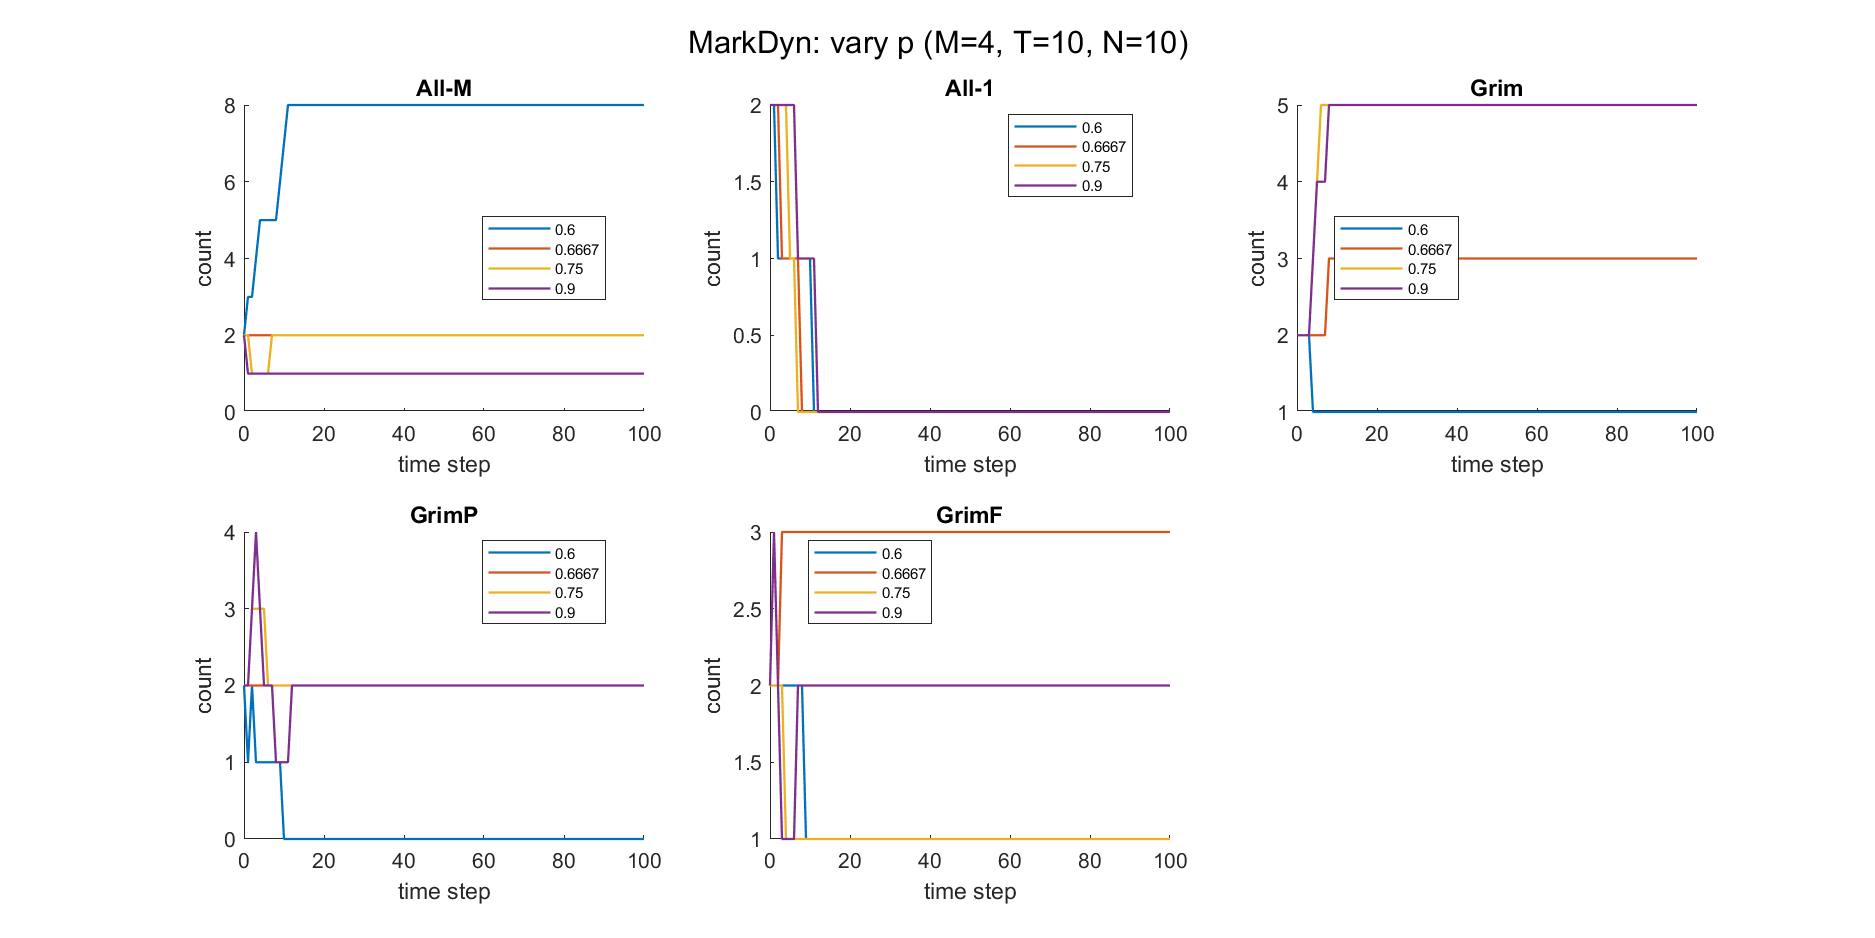
\includegraphics[width=\textwidth]{figures3/mark_overlay_vary_p}
  \label{fig:v3_mark_vary_p}
\end{figure}

\begin{figure}[H]
  \centering
  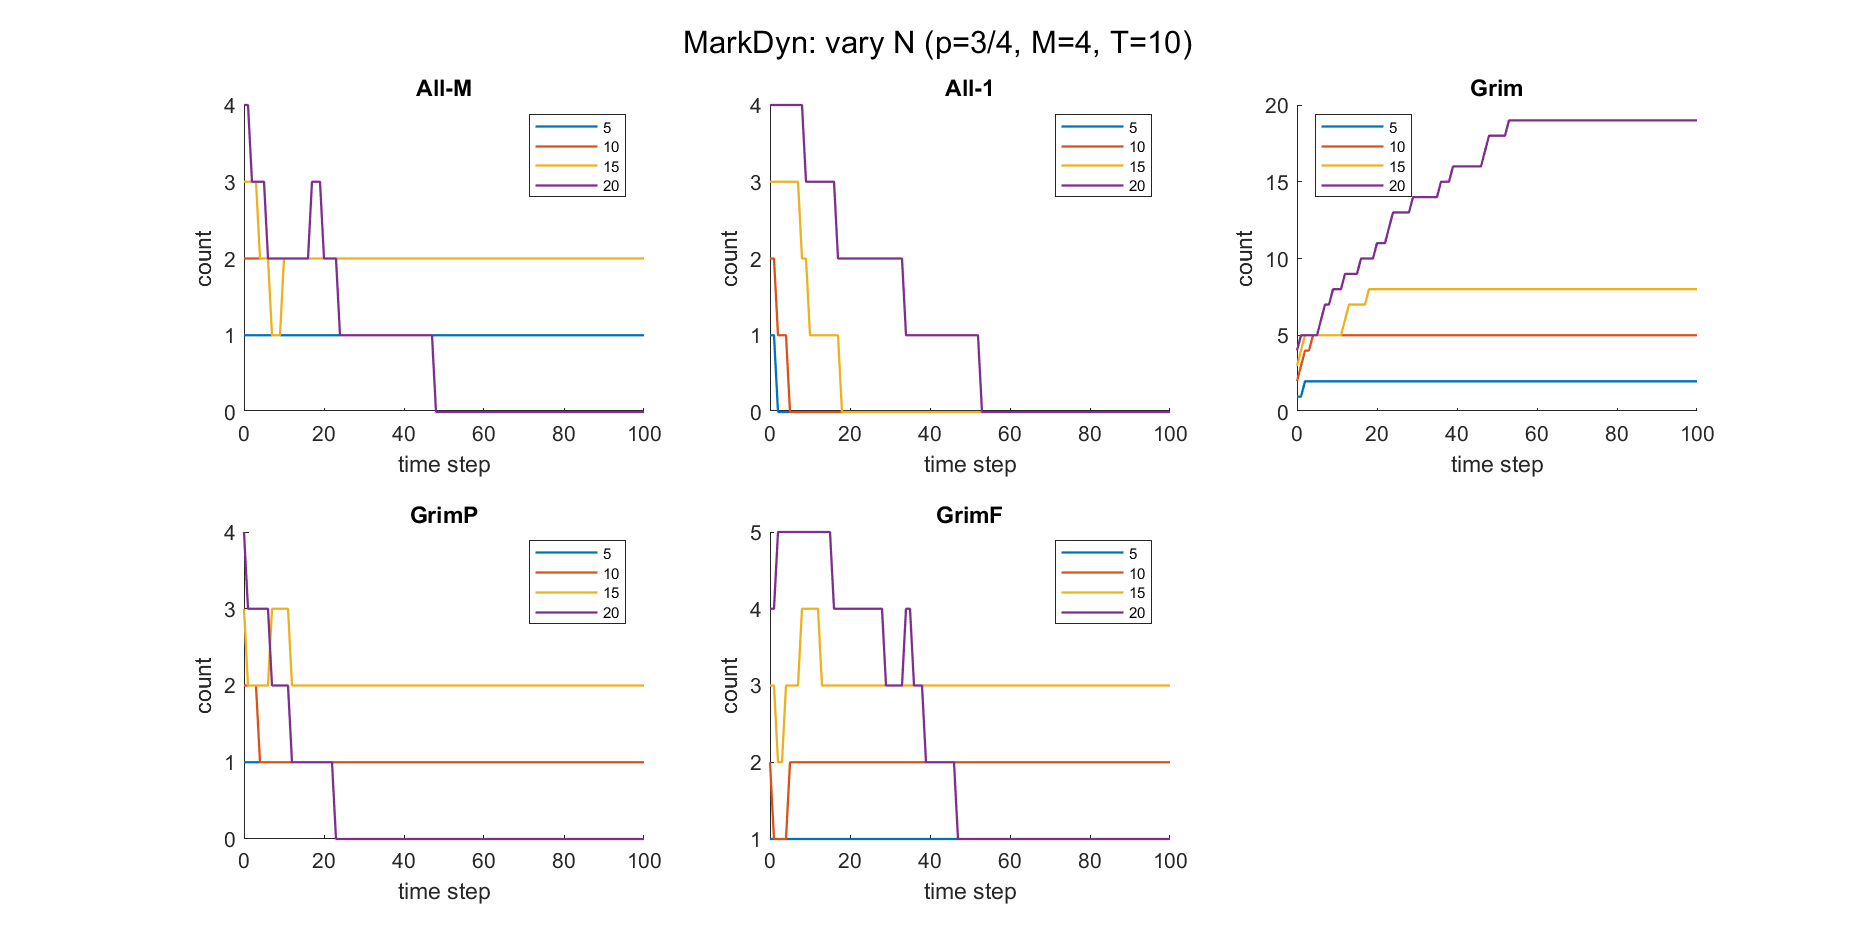
\includegraphics[width=\textwidth]{figures3/mark_overlay_vary_N}
  \label{fig:v3_mark_vary_N}
\end{figure}

\begin{figure}[H]
  \centering
  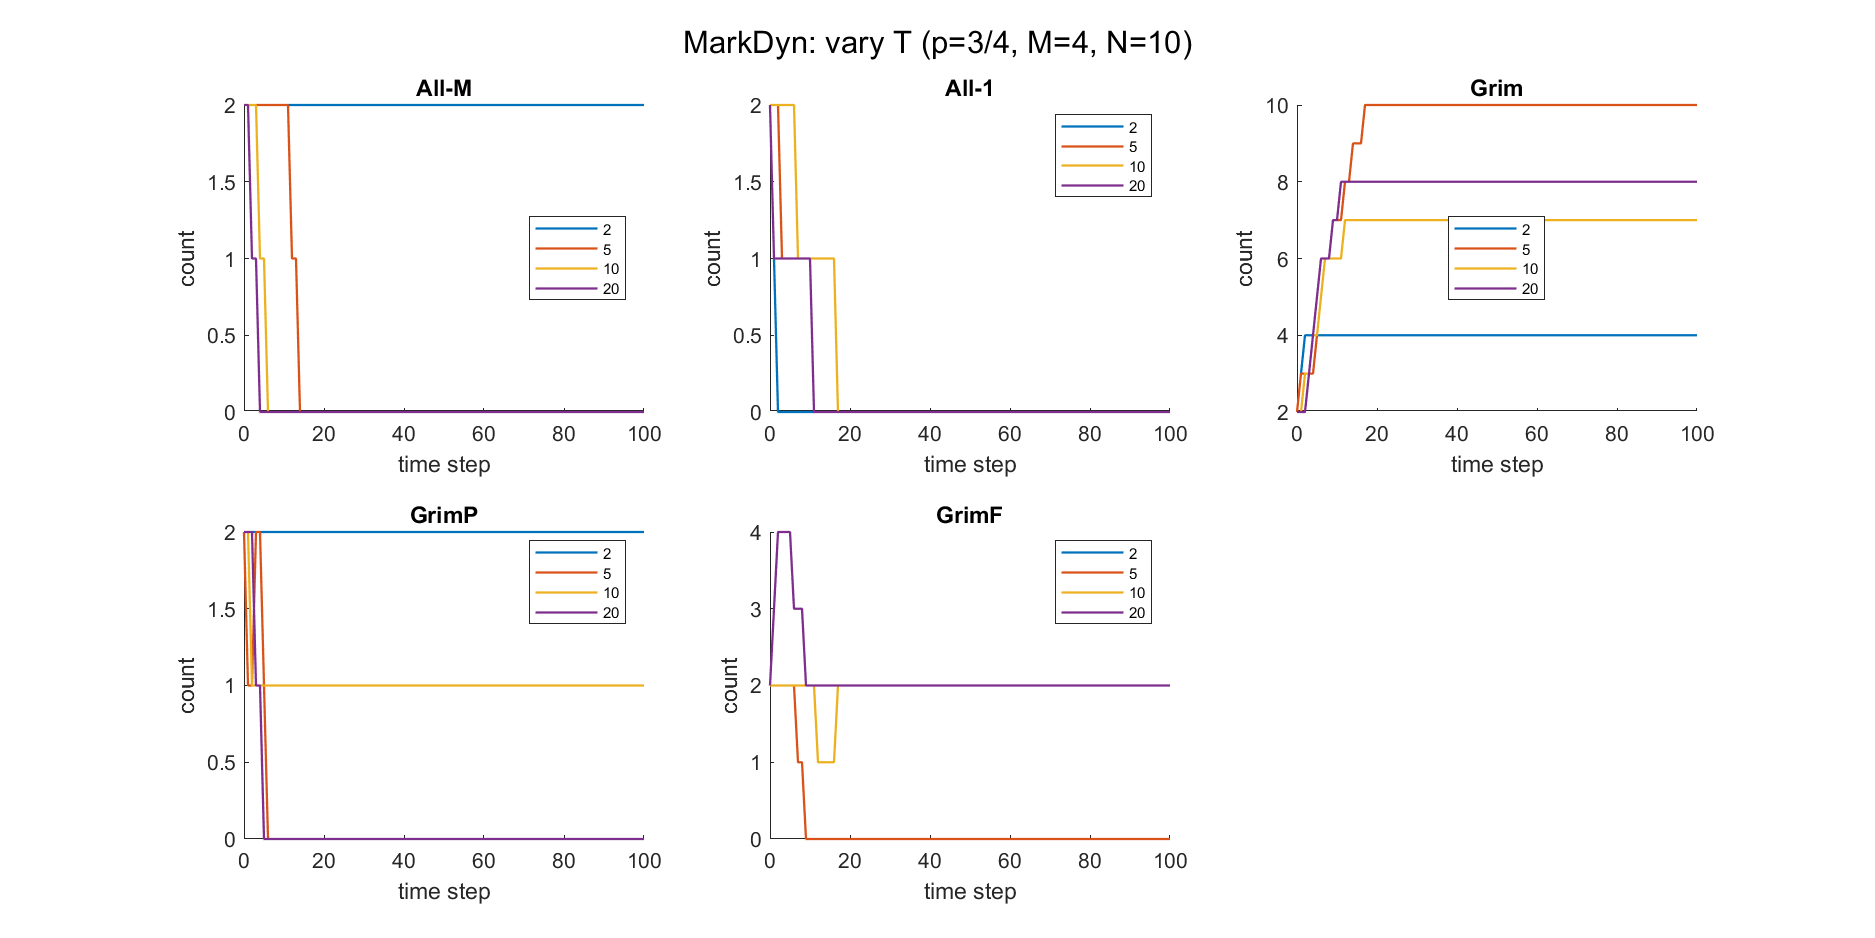
\includegraphics[width=\textwidth]{figures3/mark_overlay_vary_T}
  \label{fig:v3_mark_vary_T}
\end{figure}

\begin{figure}[H]
  \centering
  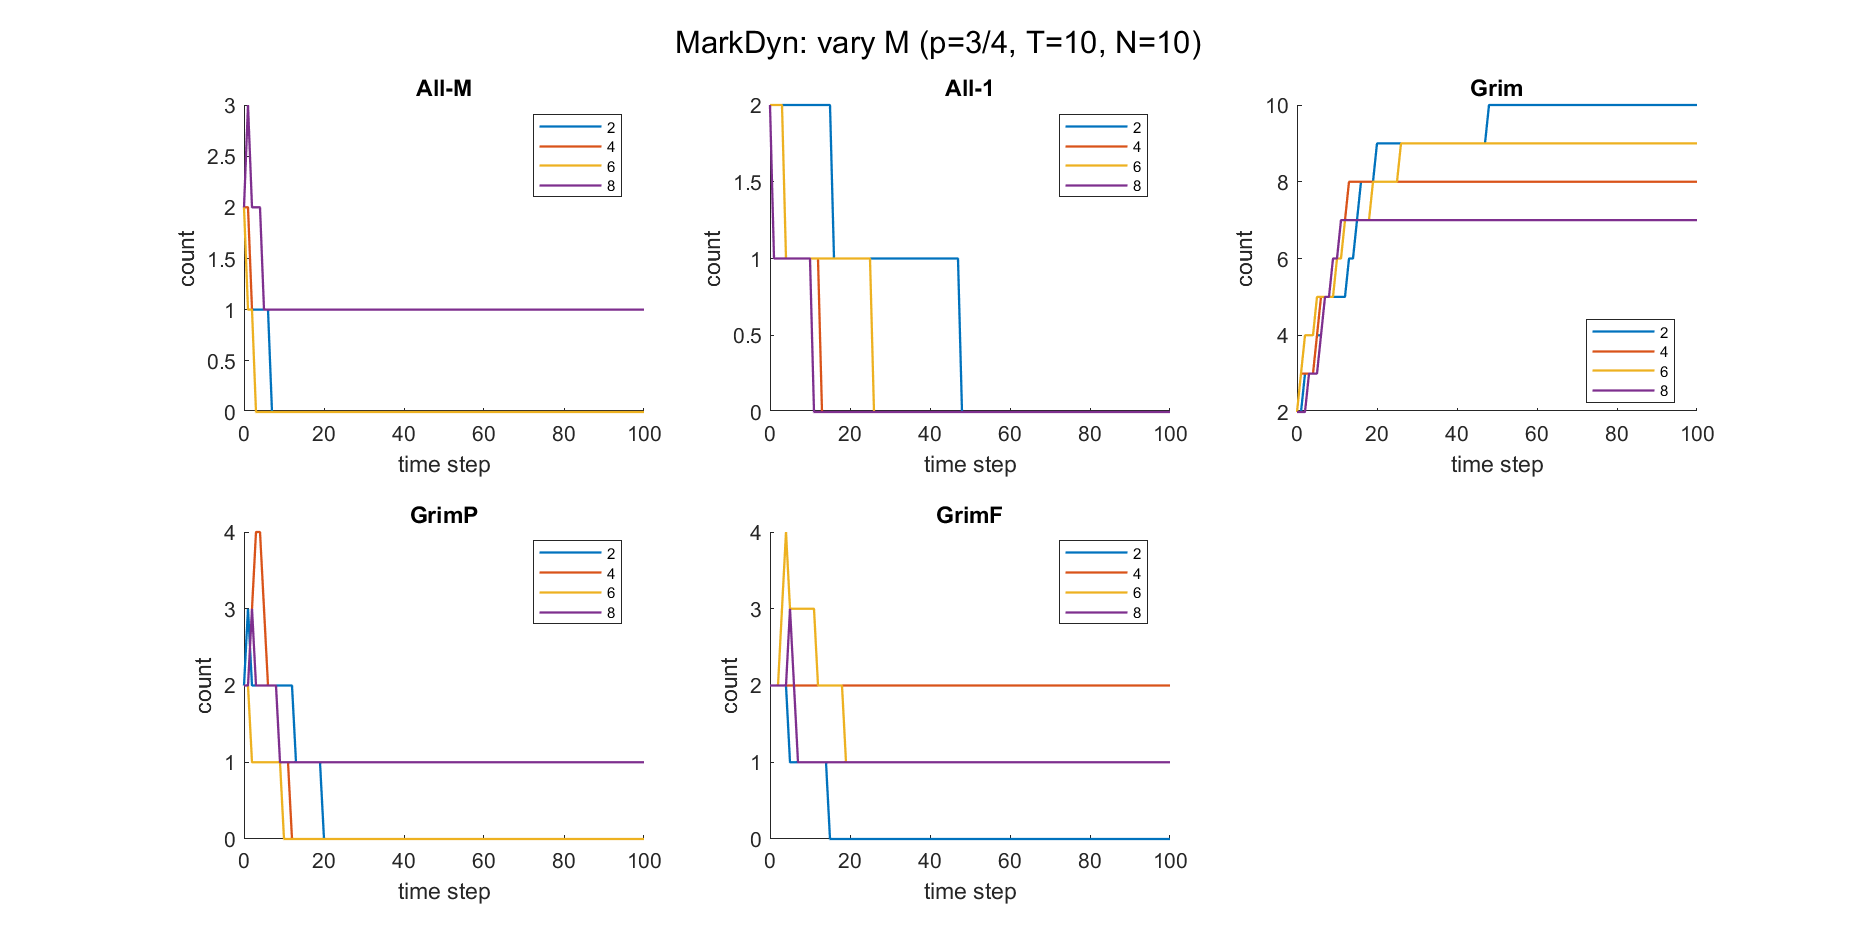
\includegraphics[width=\textwidth]{figures3/mark_overlay_vary_M}
  \label{fig:v3_mark_vary_M}
\end{figure}

\subsection{Connection to Learning Theory (Variation 3)}

In the five-strategy ISC context:
\begin{itemize}
  \item \textbf{Evolutionary.} The four cooperating strategies are
        \emph{evolutionarily neutral} relative to each other on $\mathcal{F}$.
        Natural selection acts only on the All-$1$/cooperator axis, with threshold $p^*=2/3$.
  \item \textbf{Learning.} A rational learner will reinforce any cooperating
        strategy over All-$1$ when $p<2/3$ (cooperation yields $TM$ vs.\ $T$).
        Among cooperating strategies, reinforcement is indifferent; the internal
        mix is determined by initial conditions.
  \item \textbf{Finite-population.} Under PPI, the absorbing face $\mathcal{A}$
        captures the long-run state where social learning has eliminated All-$1$.
\end{itemize}

%============================================================
\section{Variation 4: Two-Population Framework ---\\
All-\texorpdfstring{$M$}{M}, All-1, and Grim}
\label{sec:var4}
%============================================================

\subsection{Overview and Motivation}

This variation replaces the single evolving population with \emph{two} populations
that play exclusively against each other (no within-population games). Two key
motivations drive this extension:
\begin{enumerate}
  \item One-population replicator dynamics can only converge to \emph{symmetric}
        Nash equilibria~\cite{Sandholm2010}. The ISC possesses asymmetric NE
        (e.g.\ Population~1 all All-$M$, Population~2 all Grim) that are
        inaccessible to one-population dynamics.
  \item Many real interactions are inter-group: buyers vs.\ sellers, incumbents
        vs.\ entrants, immune systems vs.\ pathogens.
\end{enumerate}

The strategy set is $\{\sigma_1=\text{All-}M,\;\sigma_2=\text{All-}1,\;\sigma_3=\text{Grim}\}$
for both populations. The bimatrix game is $(C, C^\top)$, where $C$ is the same
$3\times3$ matrix as in~\cite{LK2026}:
\begin{equation}
C = \begin{pmatrix}
T M & 3(1-p)\,T & T M \\[4pt]
3p\,T & T & 3p+(T-1) \\[4pt]
T M & 3(1-p)+(T-1) & T M
\end{pmatrix}.
\end{equation}

\begin{table}[H]
\centering
\caption{Payoff matrix $C$ for $p=3/4$, $M=4$, $T=10$, Variation~4.
         Population~2 payoff matrix is $C^\top$.}
\label{tab:v4_C_p075}
\renewcommand{\arraystretch}{1.2}
\begin{tabular}{lccc}
\toprule
           & vs All-$M$ & vs All-$1$ & vs Grim \\
\midrule
All-$M$    & 40 & 7.5  & 40    \\
All-$1$    & 22.5 & 10 & 11.25 \\
Grim       & 40 & 9.75 & 40    \\
\bottomrule
\end{tabular}
\end{table}

\begin{table}[H]
\centering
\caption{Payoff matrix $C$ for $p=3/5$, $M=4$, $T=10$, Variation~4.}
\label{tab:v4_C_p060}
\renewcommand{\arraystretch}{1.2}
\begin{tabular}{lccc}
\toprule
           & vs All-$M$ & vs All-$1$ & vs Grim \\
\midrule
All-$M$    & 40 & 12  & 40    \\
All-$1$    & 18 & 10  & 10.8  \\
Grim       & 40 & 10.2 & 40   \\
\bottomrule
\end{tabular}
\end{table}

\subsection{Nash Equilibria}

\begin{definition}[Two-Population Nash Equilibrium]
A pair of mixed strategies $(\hat x, \hat y)$ with $\hat x,\hat y\in\Delta_3$
is a NE of $(C,C^\top)$ iff
$\hat x^\top C\hat y \geq x^\top C\hat y$ for all $x$ and
$\hat y^\top C^\top\hat x \geq y^\top C^\top\hat x$ for all $y$.
\end{definition}

\begin{proposition}[Asymmetric NE Family]\label{prop:v4_NEfamily}
For every $M\in\{3,4,\ldots\}$, large $T$, and any $a',a''\in[0,1]$:
\[
  \bigl((1-a',\,0,\,a'),\;(1-a'',\,0,\,a'')\bigr)
\]
is a NE of the two-population ISC. This includes genuinely \emph{asymmetric} NE
such as $(e_1,e_3)$ (Pop~1 all All-$M$, Pop~2 all Grim).
\end{proposition}

\begin{proposition}[Symmetric NE]
The symmetric NE $(\hat x,\hat x)$ of the two-population ISC coincide exactly
with the NE of the one-population game: all $(1-a',0,a')$ profiles,
$((0,1,0),(0,1,0))$ iff $p\geq 2/3$, and the mixed NE from~\cite{LK2026}.
\end{proposition}

\begin{example}[$M=4$, $T=10$, $p=3/4$]
NE include: all pairs $((1-a',0,a'),(1-a'',0,a''))$ for $a',a''\in[0,1]$,
plus the symmetric mixed NE
$\bigl((\tfrac{1}{8},\tfrac{7}{8},0),(\tfrac{1}{8},\tfrac{7}{8},0)\bigr)$.
\end{example}

\subsection{Two-Population Replicator Dynamics}

Let $x(t)=(x_1,x_2,x_3)$ and $y(t)=(y_1,y_2,y_3)$ be the strategy frequency
vectors of Population~1 and Population~2. Fitness of strategy $m$ in Population~1
is $(Cy)_m$; in Population~2 it is $(C^\top x)_m$. The two-population
replicator equations are:
\begin{align}
  \dot x_m &= x_m\bigl((Cy)_m - x^\top Cy\bigr), \label{eq:v4_rep1}\\
  \dot y_m &= y_m\bigl((x^\top C)_m - x^\top Cy\bigr). \label{eq:v4_rep2}
\end{align}
The system conserves the simplices $\Delta_3^x$ and $\Delta_3^y$ separately.
Setting $y=x$ recovers the standard one-population replicator.

\begin{proposition}[Cooperative Face Always Stable]
For every $M\geq 4$ and large $T$, the entire face
$\mathcal{F}=\{(x,y):x_2=y_2=0\}$ is stable in both transverse directions.
The eigenvalue for All-$1$ invasion of Population~1 is:
\[
  \lambda_{x_2} \approx T[1-M+(3p-1)b] \leq -1 < 0,
\]
for $y^*=(1-b,0,b)$ and $M\geq 4$. Similarly for Population~2. This is
\emph{stronger} than the one-population result (where $\mathcal{F}$ was only
neutrally stable).
\end{proposition}

\begin{proposition}[Threshold Preserved]
The critical threshold $p^*=2/3$ for All-$1$ stability is preserved:
\begin{itemize}
  \item $p>2/3$: All-$1$ is stable in both populations simultaneously.
  \item $p<2/3$: All-$1$ is unstable; the system converges to $\mathcal{F}$.
\end{itemize}
\end{proposition}

\subsubsection*{Phase Portraits and Sensitivity}

\begin{figure}[H]
  \centering
  \begin{subfigure}[b]{0.48\textwidth}
    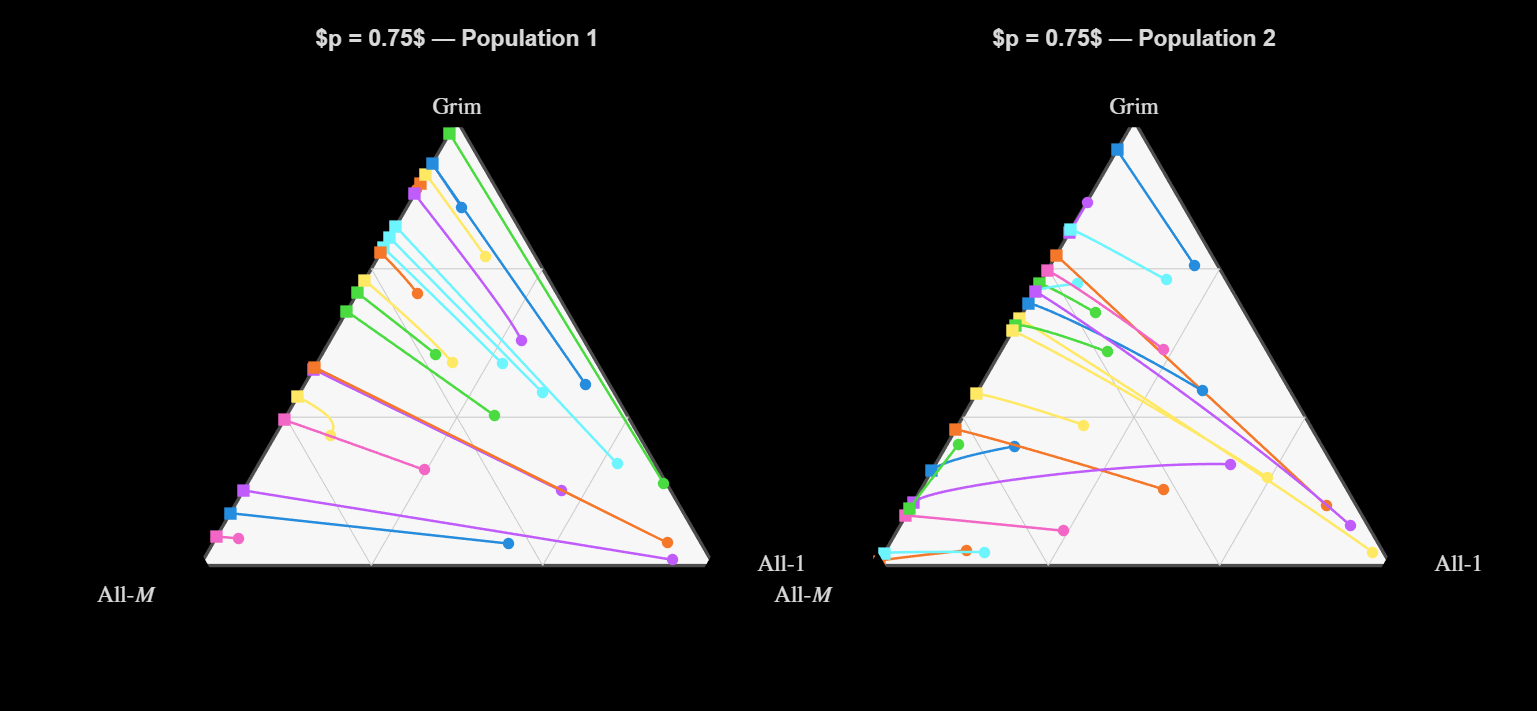
\includegraphics[width=\textwidth]{figures4/rep_phase_p075}
    \caption{$p=3/4$.}
  \end{subfigure}
  \hfill
  \begin{subfigure}[b]{0.48\textwidth}
    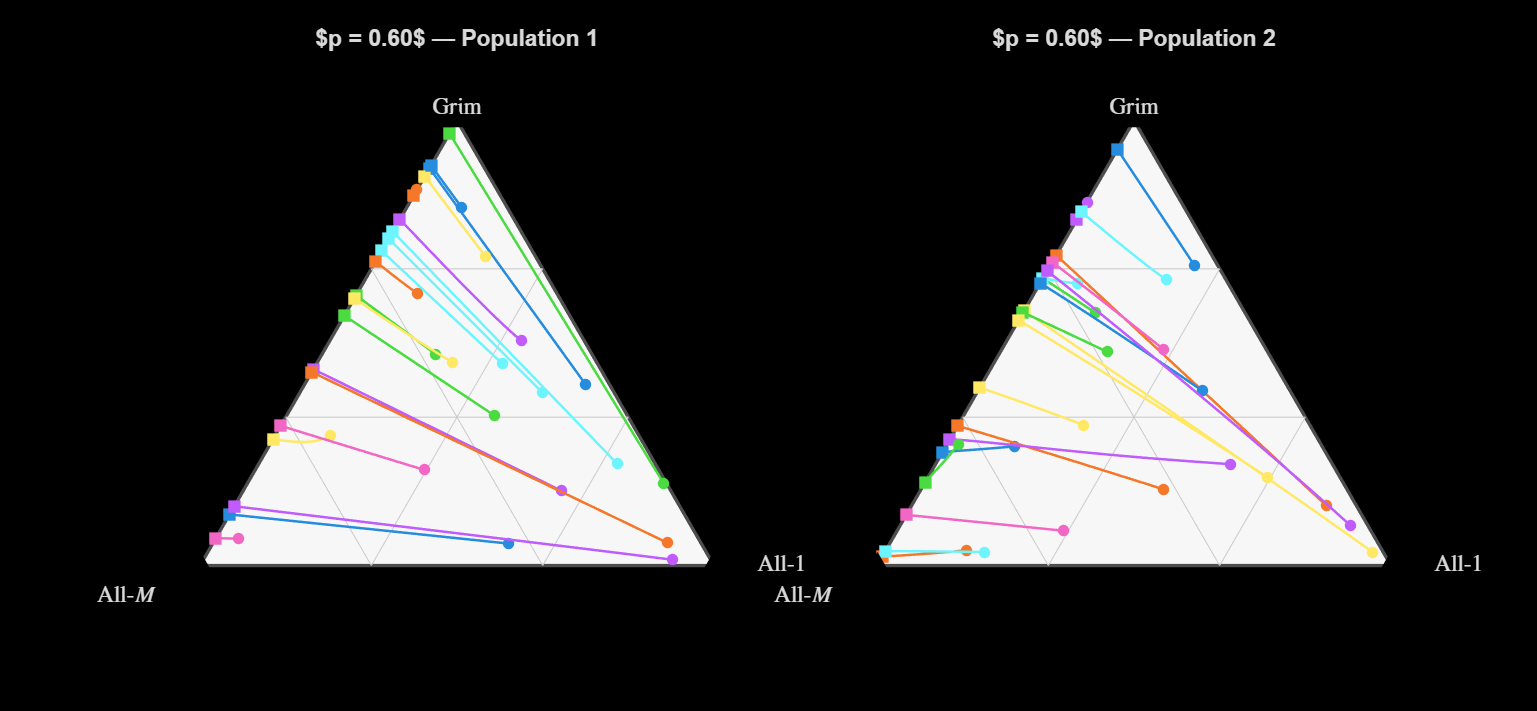
\includegraphics[width=\textwidth]{figures4/rep_phase_p060}
    \caption{$p=3/5$.}
  \end{subfigure}
  \caption{Phase portraits of the two-population replicator dynamics, Variation~4
           ($M=4$, $T=10$). Solid: Population~1. Dashed: Population~2.}
  \label{fig:v4_phase_both}
\end{figure}

\begin{figure}[H]
  \centering
  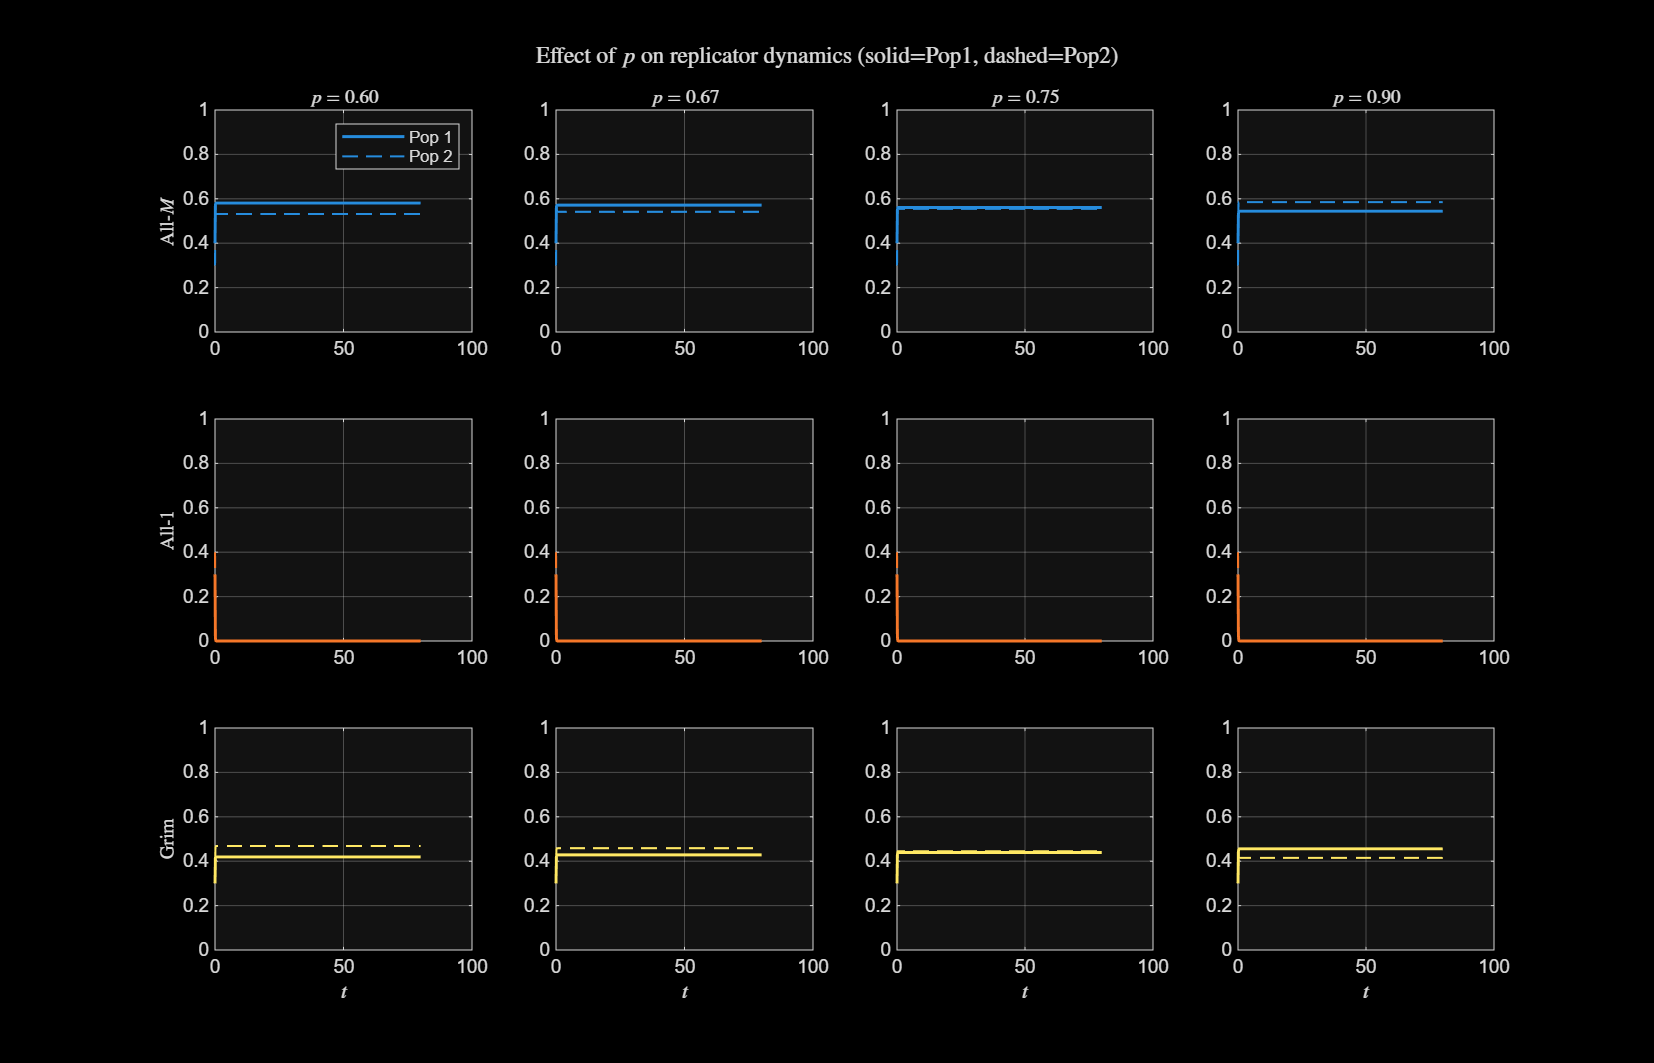
\includegraphics[width=\textwidth]{figures4/rep_overlay_vary_p}
  \caption{Effect of $p\in\{3/5,2/3,3/4,9/10\}$ on two-population replicator dynamics,
           Variation~4 ($M=4$, $T=10$).}
  \label{fig:v4_rep_vary_p}
\end{figure}

\begin{figure}[H]
  \centering
  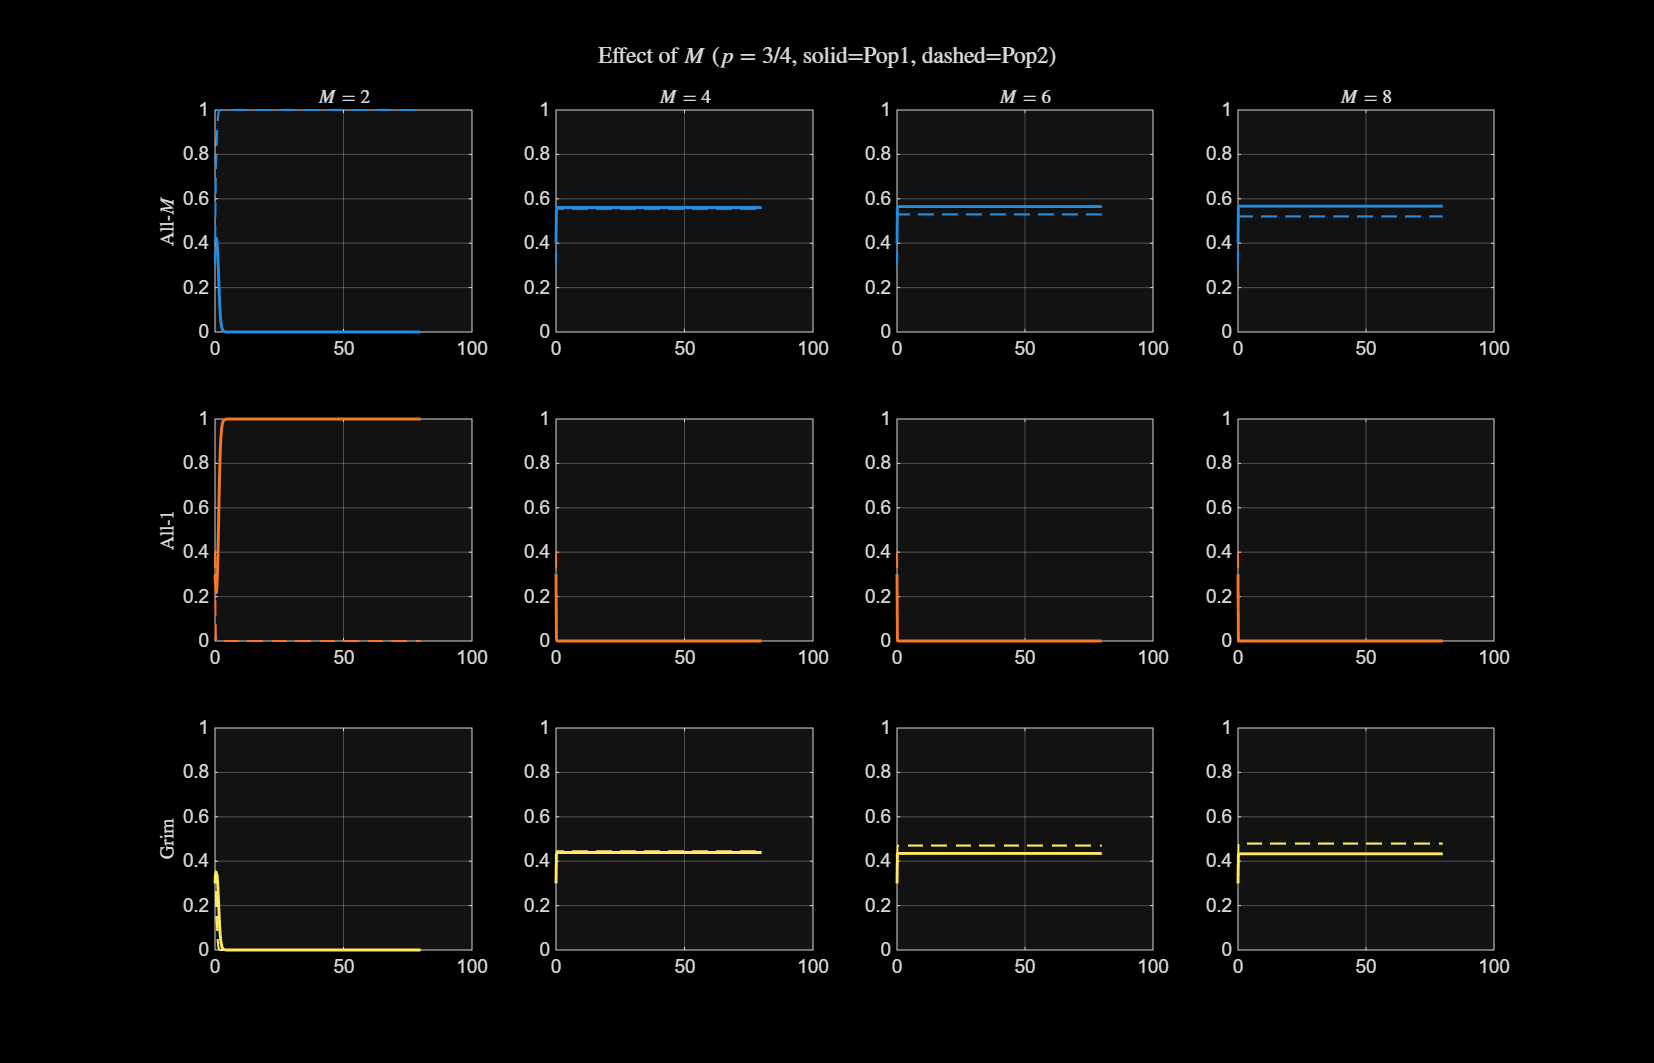
\includegraphics[width=\textwidth]{figures4/rep_overlay_vary_M}
  \caption{Effect of $M\in\{2,4,6,8\}$ on two-population replicator dynamics,
           Variation~4 ($p=3/4$, $T=10$).}
  \label{fig:v4_rep_vary_M}
\end{figure}

\begin{figure}[H]
  \centering
  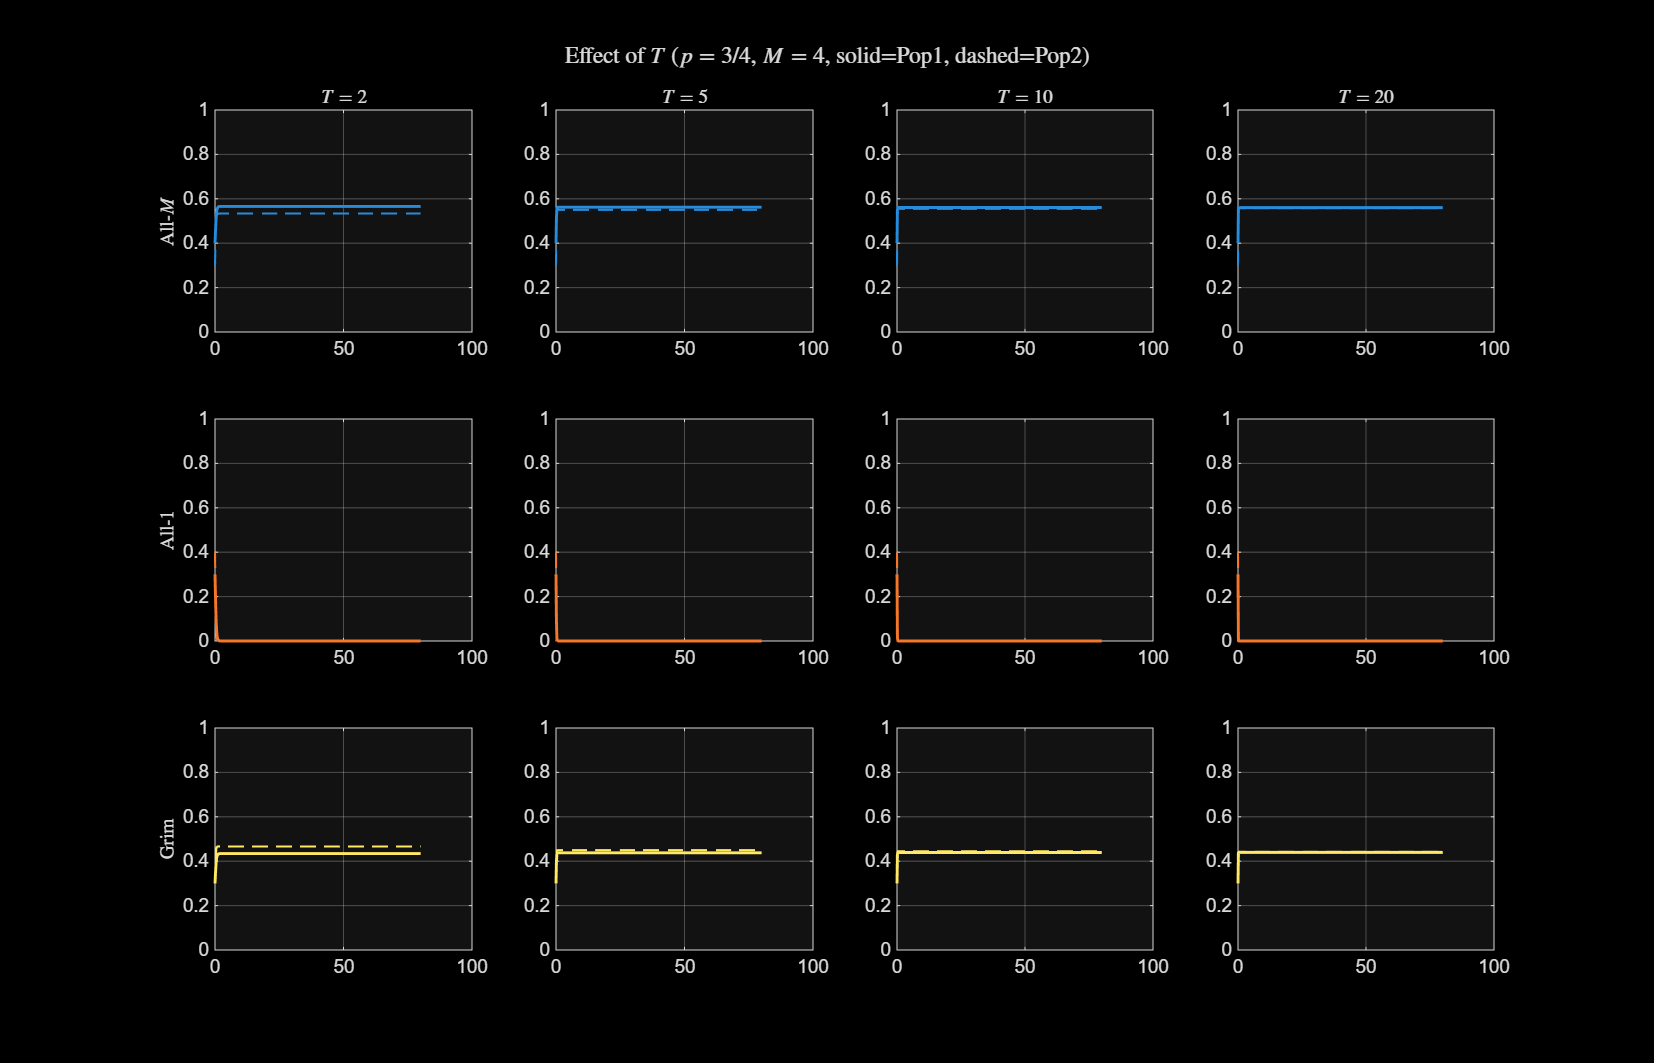
\includegraphics[width=\textwidth]{figures4/rep_overlay_vary_T}
  \caption{Effect of $T\in\{2,5,10,20\}$ on two-population replicator dynamics,
           Variation~4 ($p=3/4$, $M=4$).}
  \label{fig:v4_rep_vary_T}
\end{figure}

\subsection{Evolutionary Stable Strategies}

\begin{proposition}[Two-Population ESS]
\begin{enumerate}
  \item All-$1$ is the unique two-population ESS, iff $p>2/3$.
  \item Asymmetric NE such as $(e_1,e_3)$ are \emph{not} two-population ESS,
        because the strict ESS condition fails at equal payoffs $TM=TM$.
  \item No interior point of $\mathcal{F}$ is an ESS.
\end{enumerate}
\end{proposition}

\subsection{Two-Population Markov Chain}

The population state is $(\mathbf{s},\mathbf{t})$ where $\mathbf{s}\in\mathbb{Z}_{\geq0}^3$
with $\sum_m s_m=N_1$ and $\mathbf{t}$ with $\sum_n t_n=N_2$. Per-player payoffs:
\begin{align}
  q_m^{(1)}(\mathbf{s},\mathbf{t}) &= \sum_n t_n\,C(m,n), \\
  q_n^{(2)}(\mathbf{s},\mathbf{t}) &= \sum_m s_m\,C(m,n).
\end{align}

\begin{proposition}[Absorbing States]\label{prop:v4_abs}
For $M\geq 4$, $N_1,N_2\geq 2$, and large $T$, the absorbing states are:
\begin{enumerate}
  \item All states $(\mathbf{s},\mathbf{t})$ with $s_2=t_2=0$:
        $\mathcal{A} = \{(\mathbf{s},\mathbf{t}): s_1+s_3=N_1,\; t_1+t_3=N_2\}$.
        This face has $(N_1+1)(N_2+1)$ states.
  \item The pure All-$1$ state $((0,N_1,0),(0,N_2,0))$.
\end{enumerate}
\end{proposition}

The absorbing face $\mathcal{A}$ is \emph{two-dimensional} (independent
cooperation levels of the two populations), in contrast to the one-dimensional
$s_2=0$ face of the one-population model.

\begin{figure}[H]
  \centering
  \begin{subfigure}[b]{0.48\textwidth}
    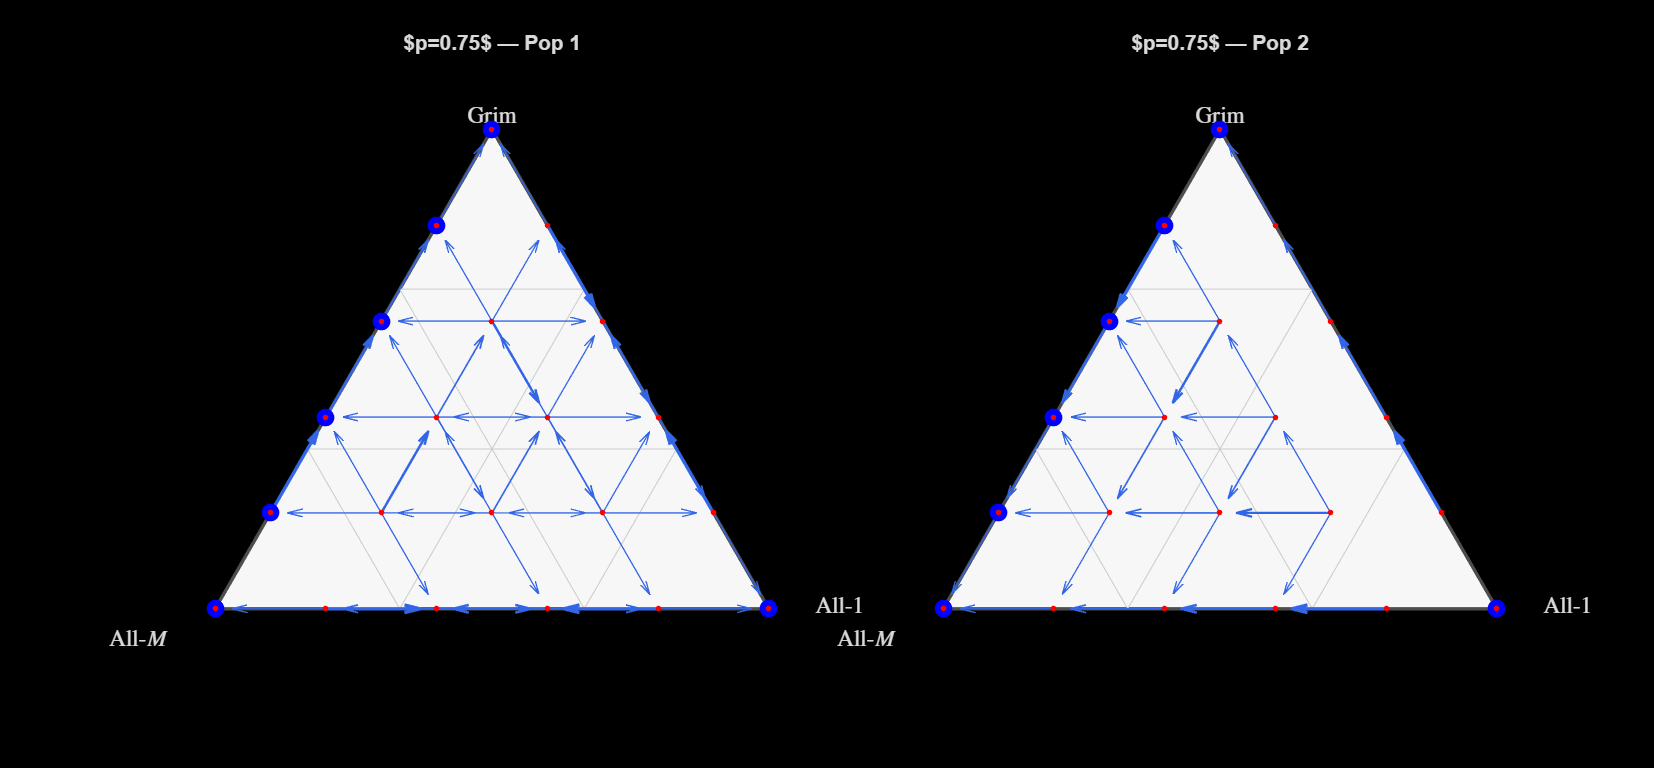
\includegraphics[width=\textwidth]{figures4/mark_stategraph_p075}
    \caption{$p=3/4$.}
  \end{subfigure}
  \hfill
  \begin{subfigure}[b]{0.48\textwidth}
    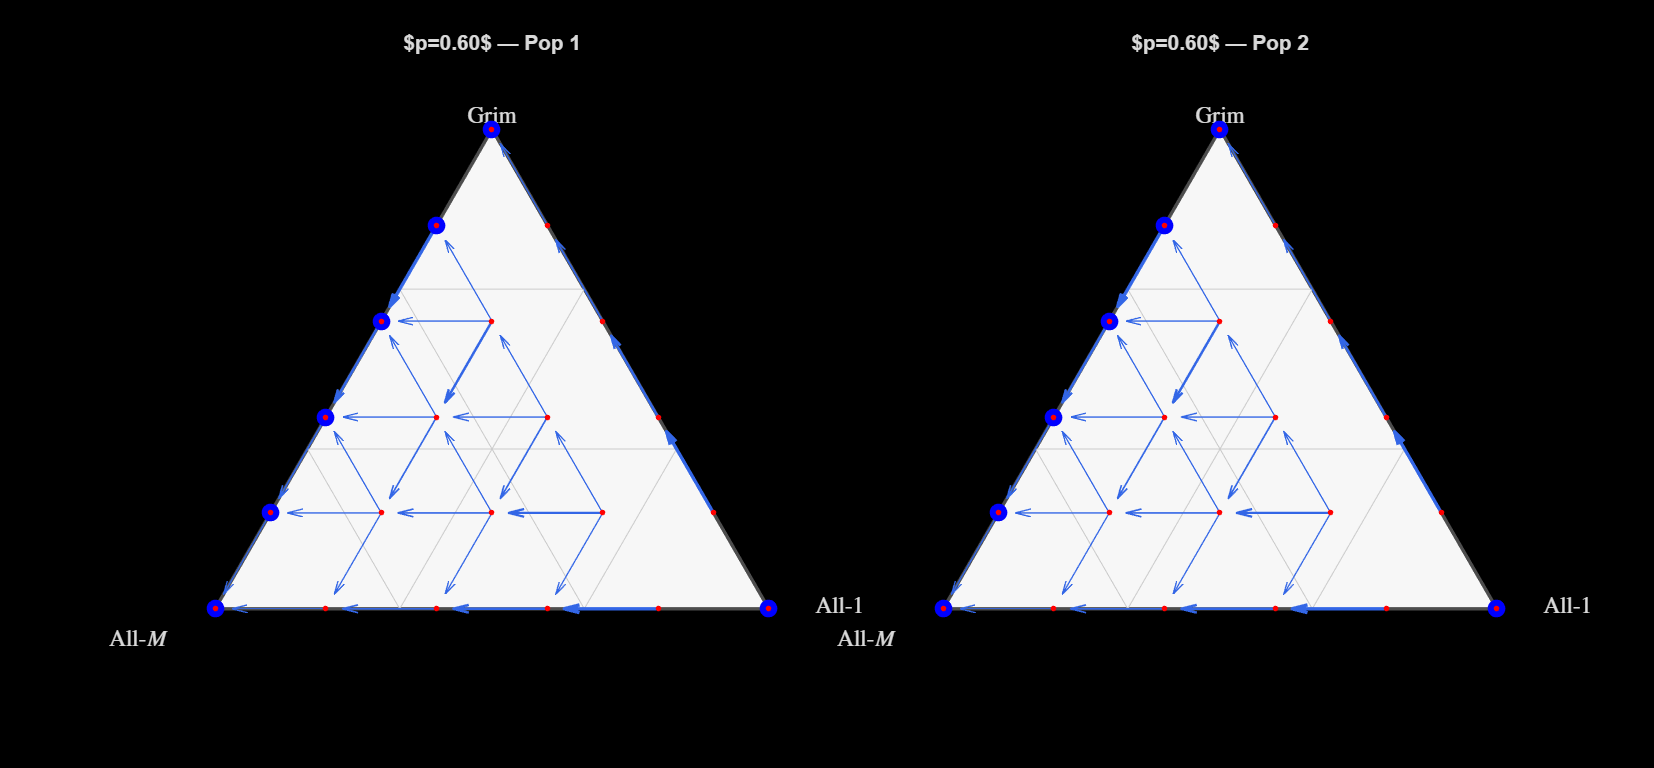
\includegraphics[width=\textwidth]{figures4/mark_stategraph_p060}
    \caption{$p=3/5$.}
  \end{subfigure}
  \caption{Two-population Markov state transition graphs, Variation~4
           ($M=4$, $T=10$, $N_1=N_2=5$).
           Blue: absorbing states. Red: transient.}
  \label{fig:v4_stategraph_both}
\end{figure}

\begin{figure}[H]
  \centering
  \begin{subfigure}[b]{0.48\textwidth}
    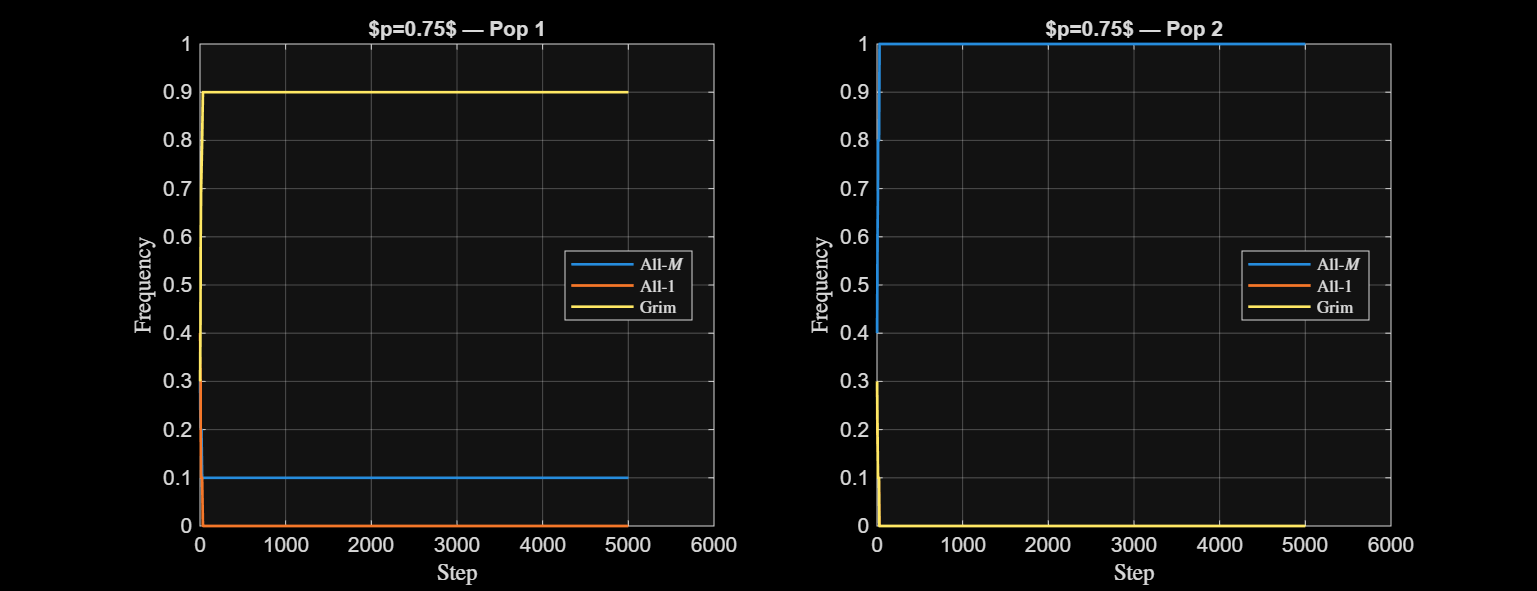
\includegraphics[width=\textwidth]{figures4/mark_timeseries_p075}
    \caption{$p=3/4$.}
  \end{subfigure}
  \hfill
  \begin{subfigure}[b]{0.48\textwidth}
    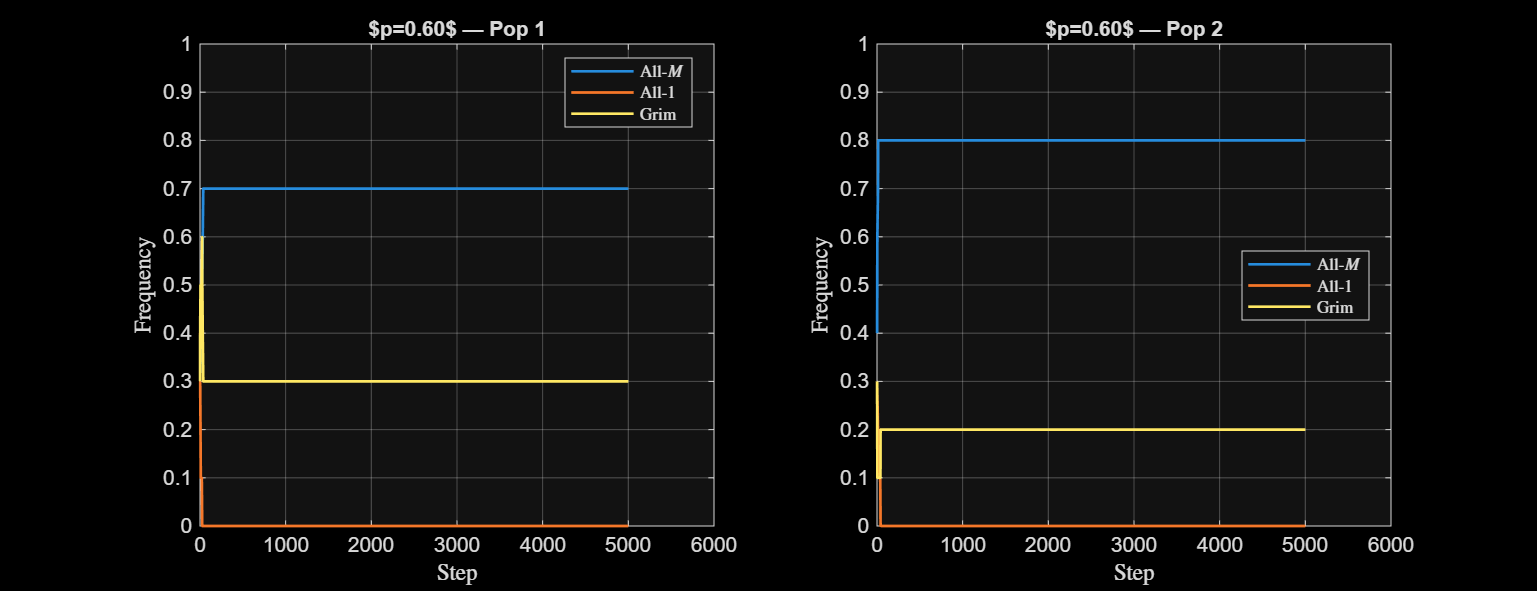
\includegraphics[width=\textwidth]{figures4/mark_timeseries_p060}
    \caption{$p=3/5$.}
  \end{subfigure}
  \caption{Two-population Markov dynamics time series, Variation~4
           ($M=4$, $T=10$, $N_1=N_2=10$, 5000 steps,
           $\mathbf{s}_0=(3,4,3)$, $\mathbf{t}_0=(4,3,3)$).
           Solid: Pop~1. Dashed: Pop~2.}
  \label{fig:v4_mark_timeseries}
\end{figure}

\begin{figure}[H]
  \centering
  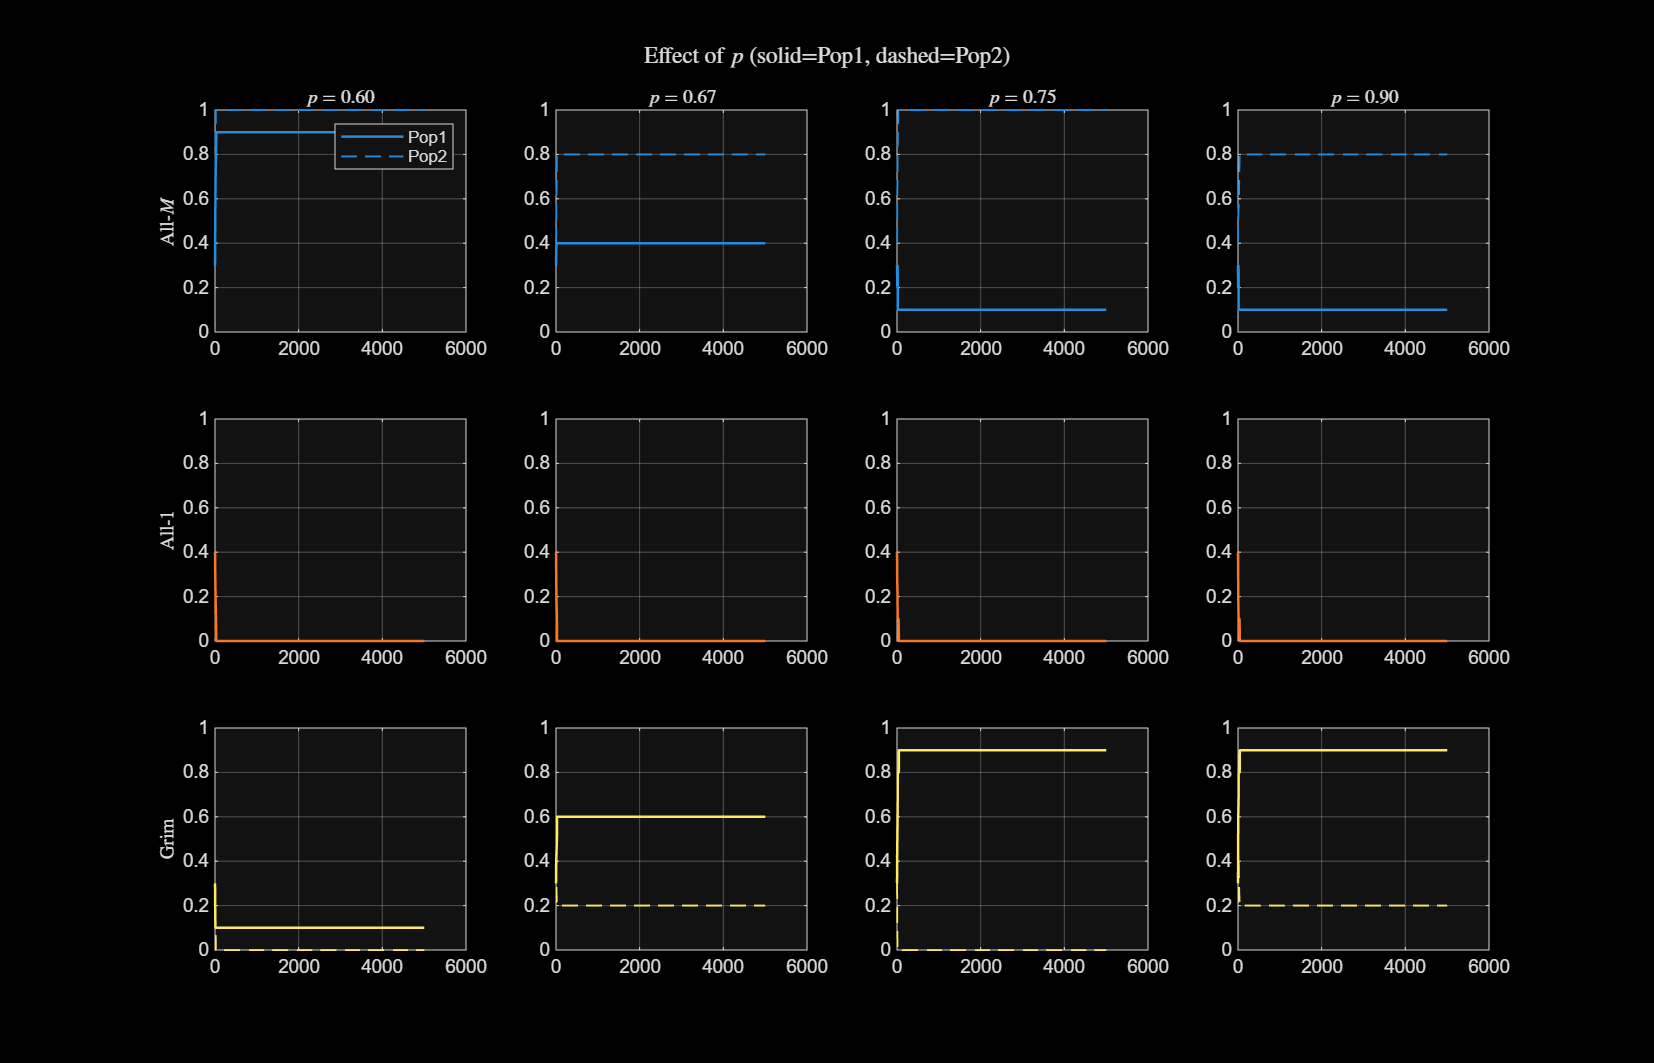
\includegraphics[width=\textwidth]{figures4/mark_overlay_vary_p}
  \caption{Effect of $p\in\{3/5,2/3,3/4,9/10\}$, Variation~4 ($M=4$, $T=10$, $N=10$).}
  \label{fig:v4_mark_vary_p}
\end{figure}

\begin{figure}[H]
  \centering
  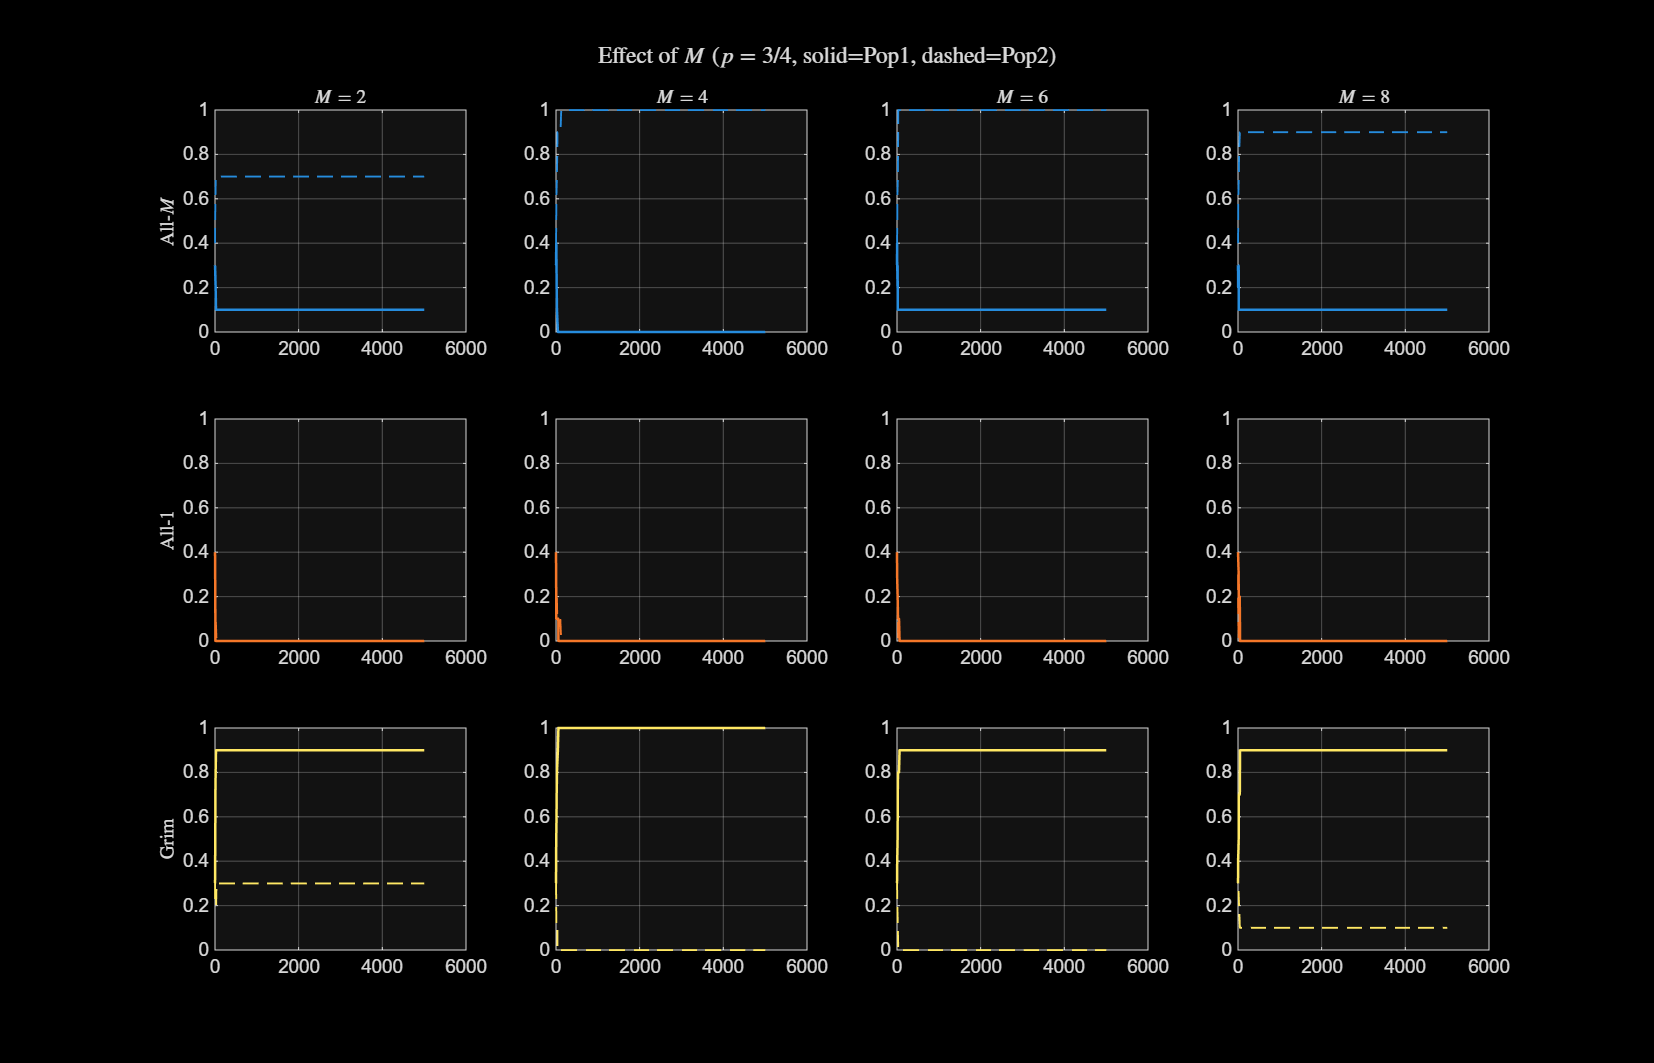
\includegraphics[width=\textwidth]{figures4/mark_overlay_vary_M}
  \caption{Effect of $M\in\{2,4,6,8\}$, Variation~4 ($p=3/4$, $T=10$, $N=10$).}
  \label{fig:v4_mark_vary_M}
\end{figure}

\begin{figure}[H]
  \centering
  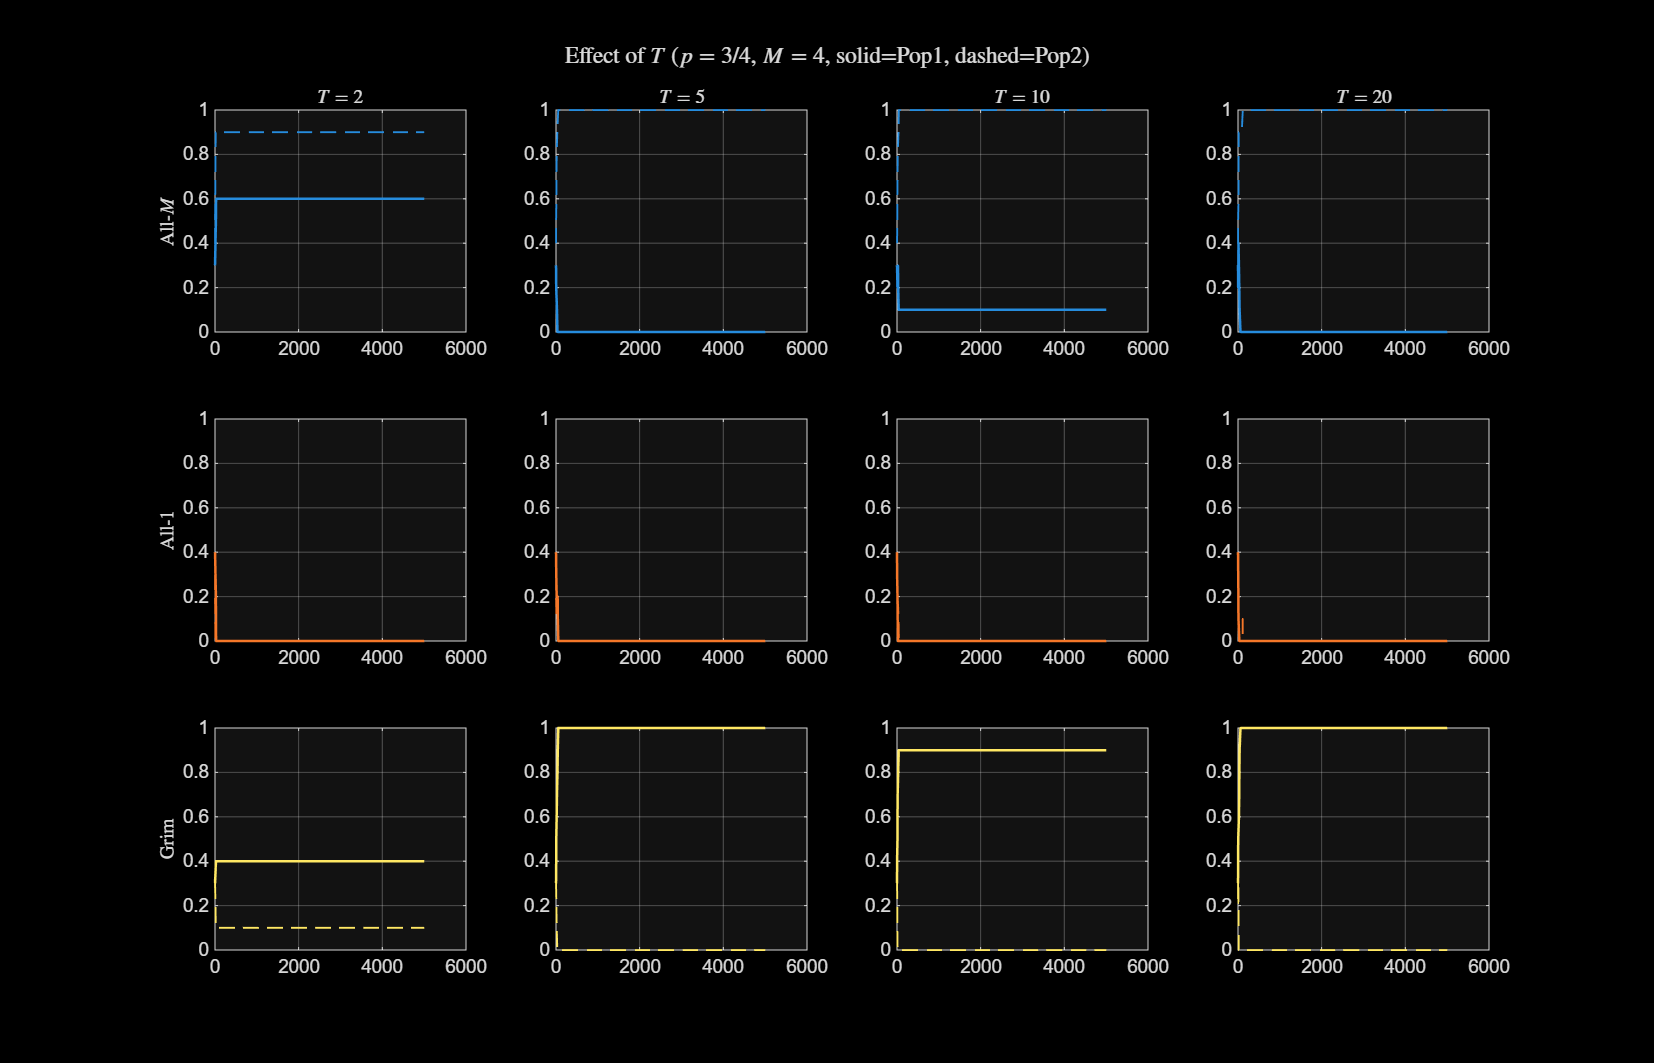
\includegraphics[width=\textwidth]{figures4/mark_overlay_vary_T}
  \caption{Effect of $T\in\{2,5,10,20\}$, Variation~4 ($p=3/4$, $M=4$, $N=10$).}
  \label{fig:v4_mark_vary_T}
\end{figure}

\begin{figure}[H]
  \centering
  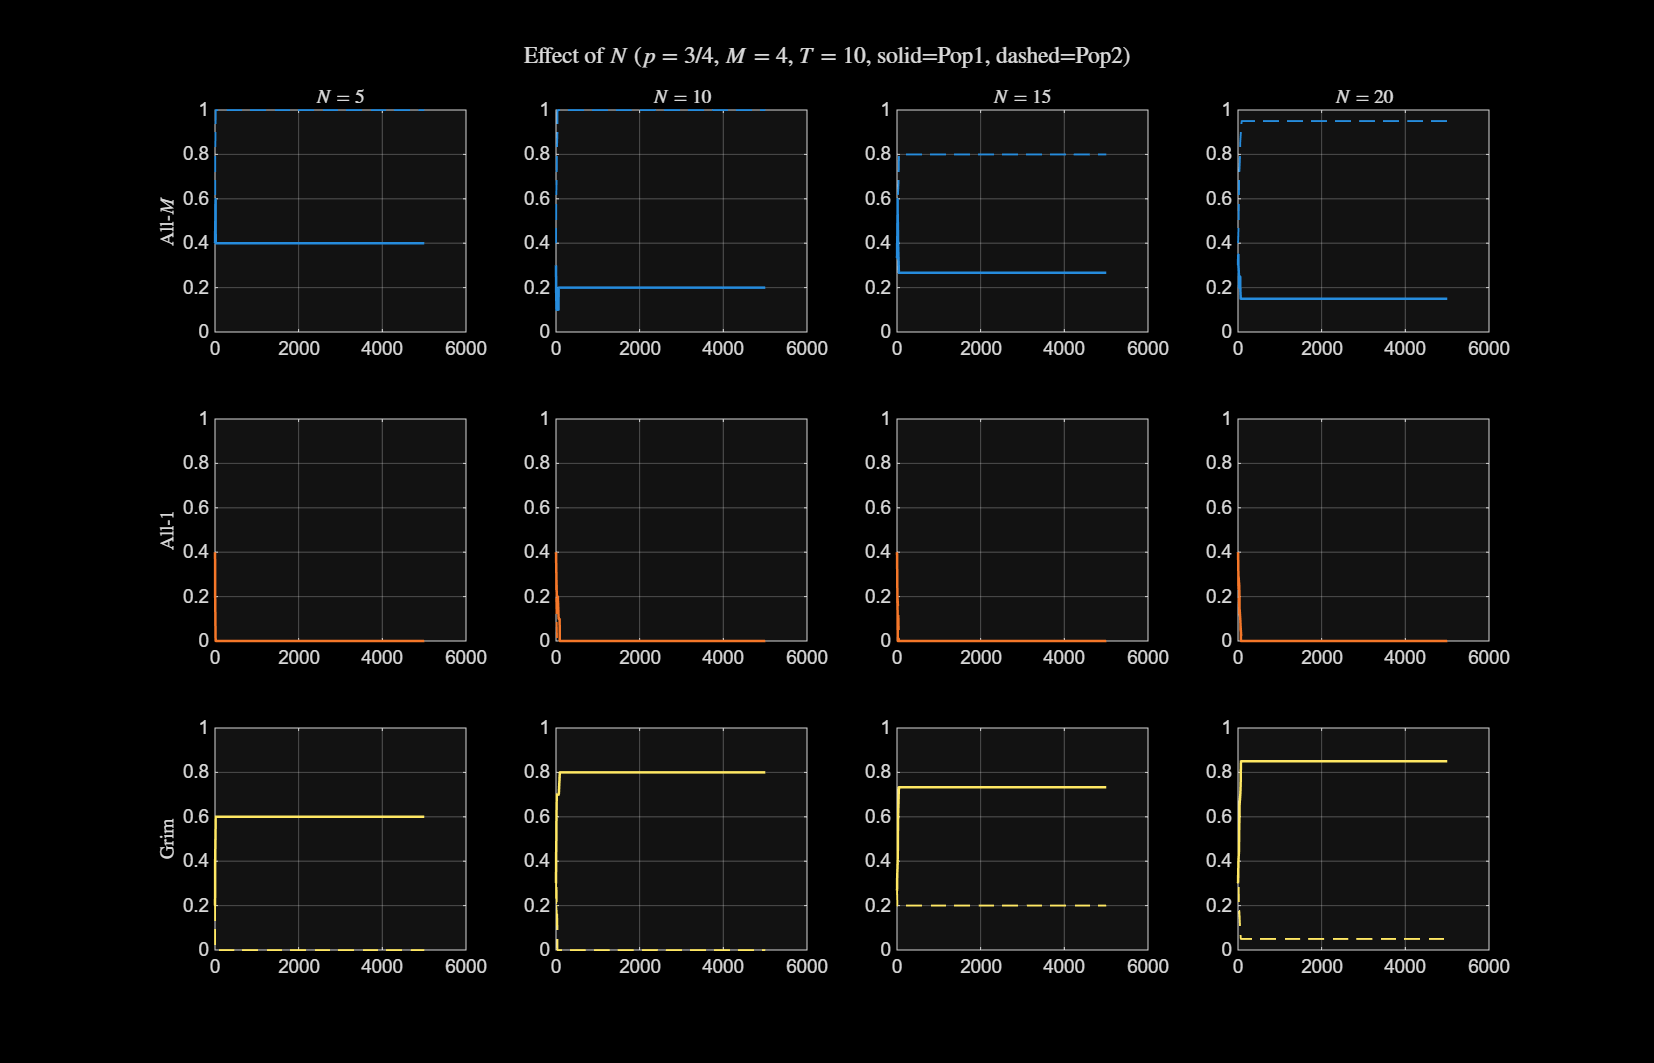
\includegraphics[width=\textwidth]{figures4/mark_overlay_vary_N}
  \caption{Effect of $N\in\{5,10,15,20\}$ ($N_1=N_2=N$),
           Variation~4 ($p=3/4$, $M=4$, $T=10$).}
  \label{fig:v4_mark_vary_N}
\end{figure}

\begin{figure}[H]
  \centering
  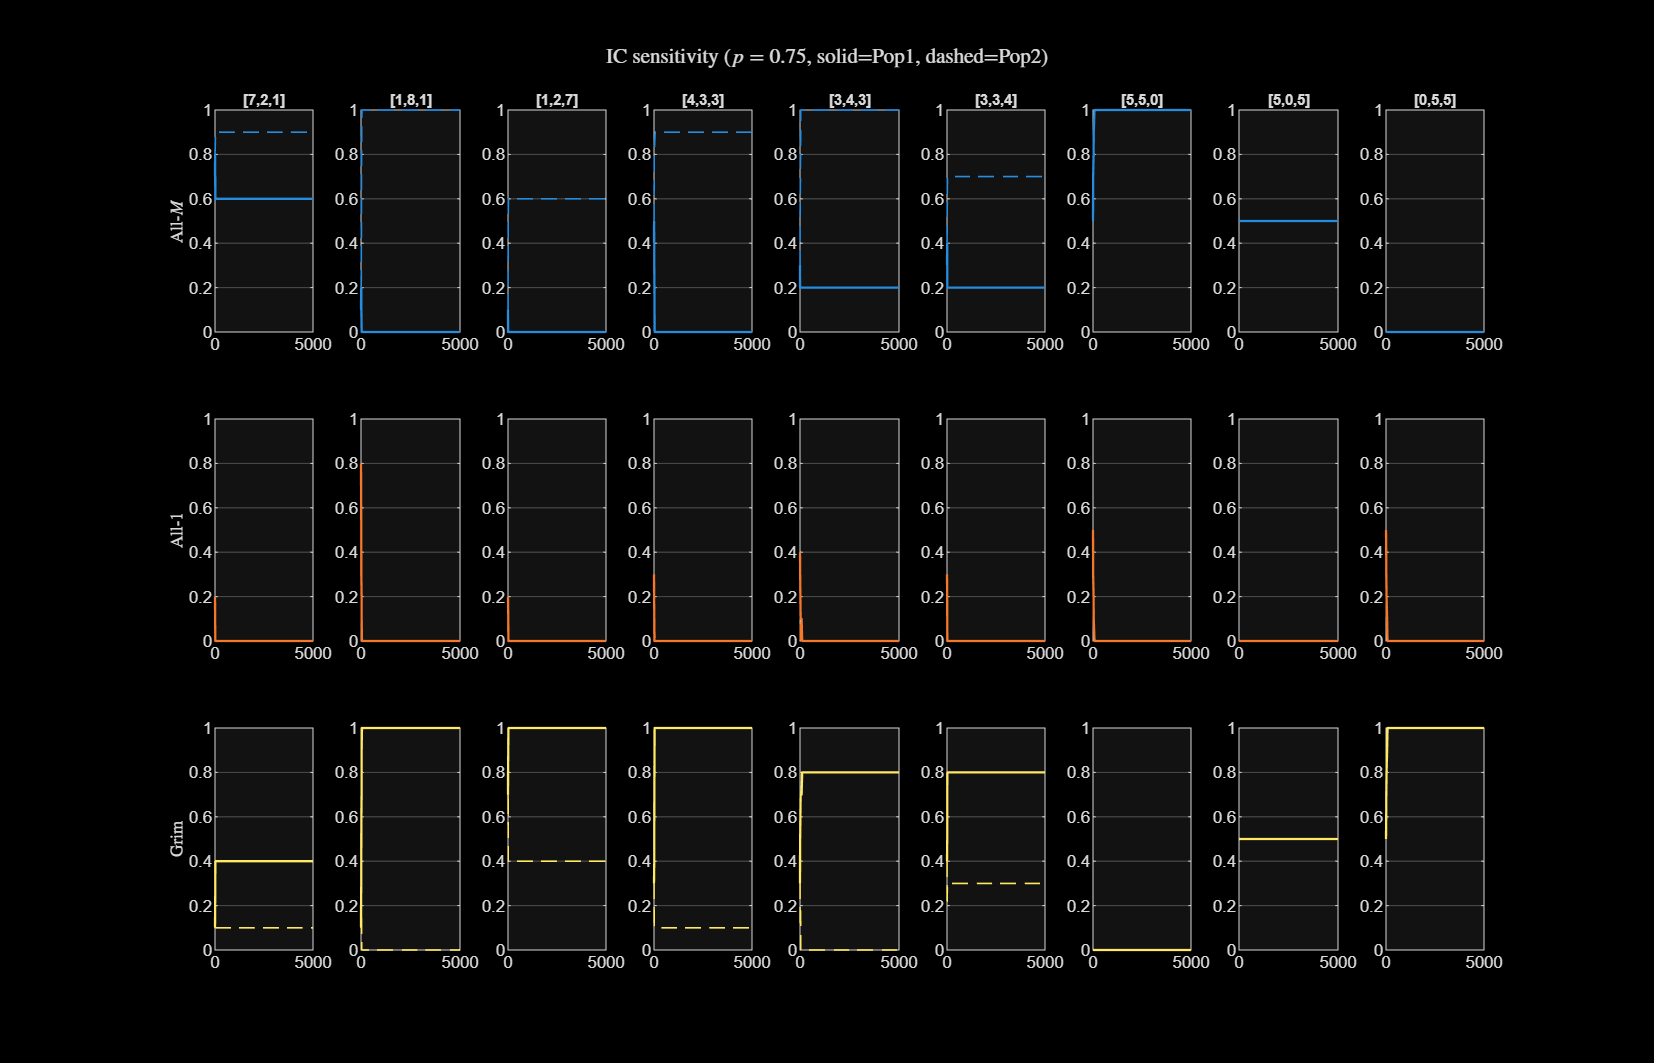
\includegraphics[width=\textwidth]{figures4/mark_overlay_vary_s0_p075}
  \caption{Initial state sensitivity ($p=3/4$, $M=4$, $T=10$, $N=10$), Variation~4.}
  \label{fig:v4_mark_s0_p075}
\end{figure}

\begin{figure}[H]
  \centering
  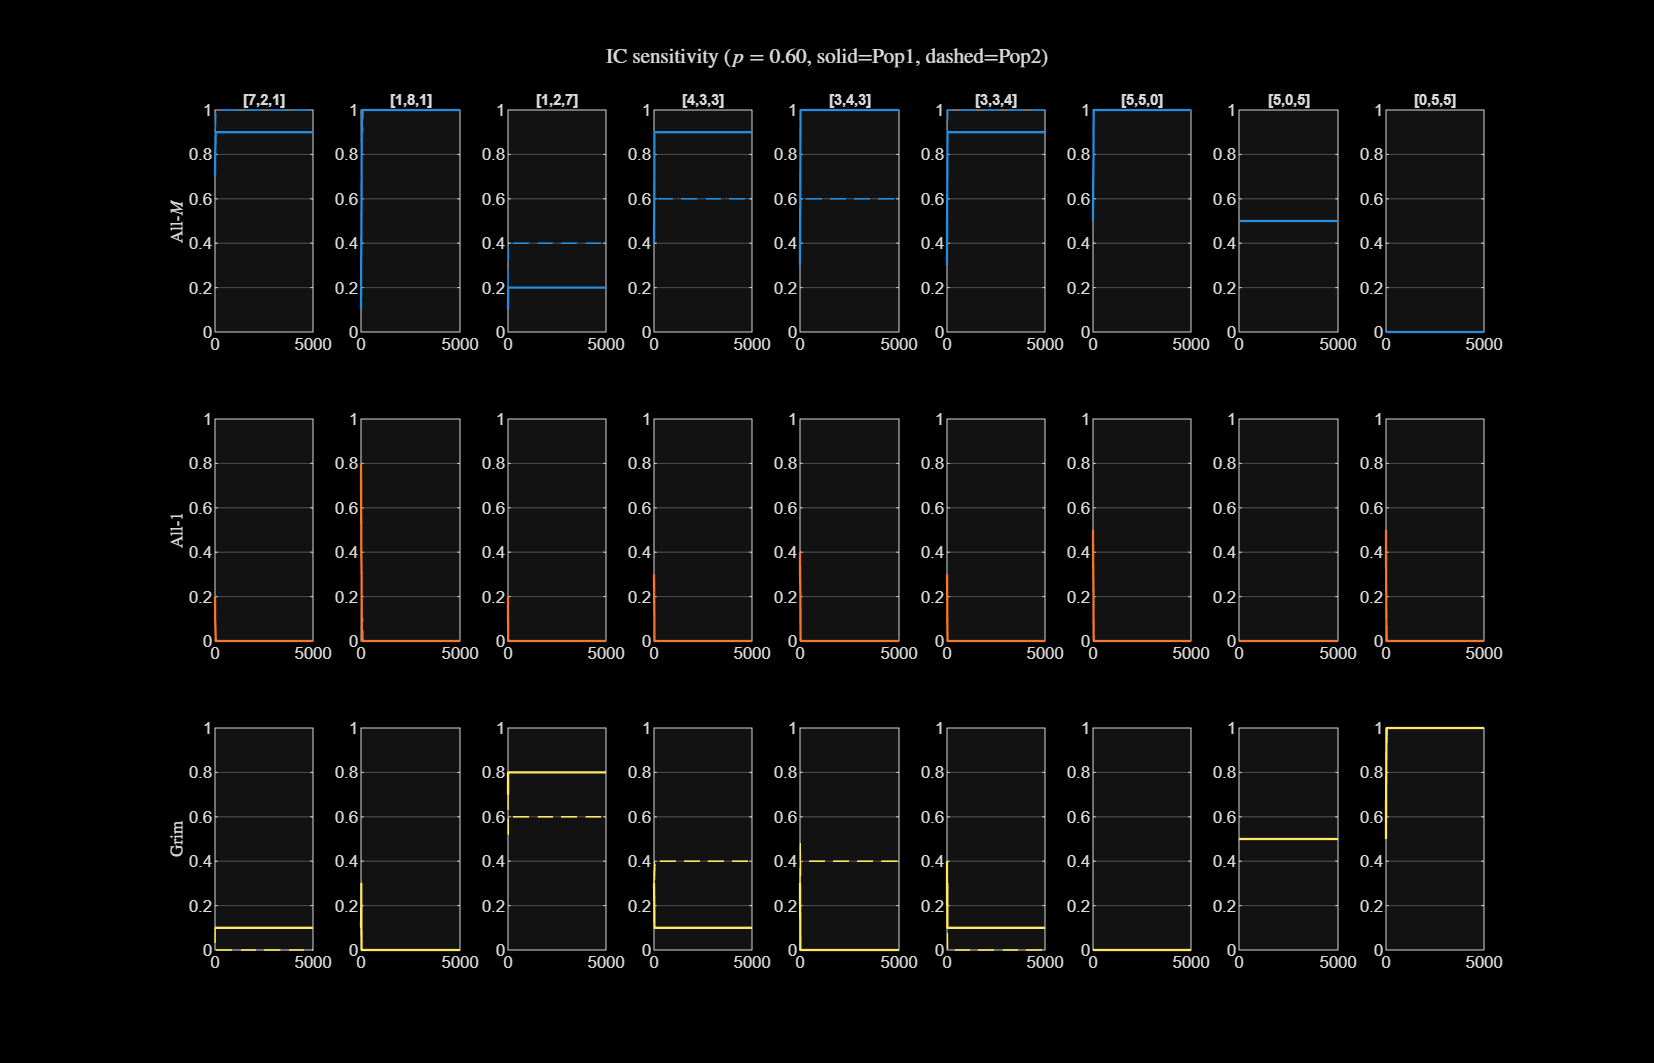
\includegraphics[width=\textwidth]{figures4/mark_overlay_vary_s0_p060}
  \caption{Initial state sensitivity ($p=3/5$, $M=4$, $T=10$, $N=10$), Variation~4.}
  \label{fig:v4_mark_s0_p060}
\end{figure}

\subsection{New Phenomena vs.\ One-Population Model}

\begin{table}[H]
\centering
\caption{Comparison: one-population vs.\ two-population ISC (Variation~4).}
\label{tab:v4_compare}
\small
\renewcommand{\arraystretch}{1.2}
\begin{tabular}{lll}
\toprule
Feature & One-population & Two-population \\
\midrule
Replicator dynamics   & $\dot x_m=x_m[(Cx)_m-x^\top Cx]$ &
                        Eqs.~\eqref{eq:v4_rep1}--\eqref{eq:v4_rep2} \\
Accessible NE         & Symmetric only & Symmetric and asymmetric \\
Absorbing face        & 1-D ($s_2=0$ line) & 2-D ($s_2=t_2=0$ face) \\
Total absorbing states & $N+1$ & $(N_1+1)(N_2+1)$ \\
Stability of $\mathcal{F}$ & Neutral (eigenvalue $= 0$) & Asymptotically stable \\
$p^*$ for All-$1$ stability & $2/3$ & $2/3$ (preserved) \\
\bottomrule
\end{tabular}
\end{table}

%============================================================
\section{Cross-Variation Remarks and Observations}
\label{sec:remarks}
%============================================================

\subsection{The Universal \texorpdfstring{$p = 2/3$}{p = 2/3} Threshold}

The critical threshold $p^* = 2/3$ appears in all four variations and governs
the stability of the all-defector equilibrium:
\begin{itemize}
  \item $p > 2/3$: the All-$1$ equilibrium is asymptotically stable (and is an
        ESS where applicable). All-$1$ can invade and resist invasion.
  \item $p < 2/3$: the All-$1$ equilibrium is unstable. Cooperating strategies
        invade All-$1$ and drive it out. The cooperative face or cooperative
        absorbing states become the long-run outcome.
  \item $p = 2/3$: a degenerate case; All-$1$ is unstable to Grim-type invasion
        in Variations~1--3.
\end{itemize}

This threshold arises mechanically from the payoff structure: against a
homogeneous All-$1$ population, a small Grim (or Grim-variant) mutant earns
$C(\text{Grim},2) - C(\text{All-}1,2) = (2-3p)$ more than the All-$1$
incumbents. The sign of this expression determines invasion success.

\subsection{Absorbing State Structure Across Variations}

The structure of absorbing states changes substantially across variations:

\begin{center}
\renewcommand{\arraystretch}{1.2}
\begin{tabular}{lll}
\toprule
Variation & Cooperator strategy & Absorbing states \\
\midrule
1 (All-$M/2$, numerical)  & All-$M/2$ & Three pure vertices only \\
2 (All-$M/2$, rigorous)   & All-$M/2$ & Three pure vertices only \\
3 (Five strategies)        & All-$M$, Grim, GrimP, GrimF & $\binom{N+3}{3}+1$ states \\
4 (Two populations)        & All-$M$, Grim & $(N_1+1)(N_2+1)+1$ states \\
\bottomrule
\end{tabular}
\end{center}

The key insight is that whenever cooperating strategies earn \emph{equal}
payoffs against each other (as in the original All-$M$/Grim pair, and in the
five-strategy and two-population extensions), the entire All-$1$-free face is
absorbing. When cooperating strategies earn \emph{unequal} payoffs in self-play
(as in Variations~1--2 with All-$M/2$), only pure vertices absorb.

\subsection{Grim and Cooperation}

Across all variations, Grim (and strategies with similar trigger structures) is
the most successful in evolutionary dynamics:
\begin{itemize}
  \item In Variations~1--2, Grim uniquely earns $TM$ in self-play (vs.\ $TM/2$
        for All-$M/2$), making it the dominant absorbing vertex and the unique
        ESS for all $p$.
  \item In Variation~3, all four cooperating strategies earn $TM$ against each
        other, but Grim best resists All-$1$ exploitation for $p > 2/3$.
  \item In Variation~4, both All-$M$ and Grim earn $TM$ against each other,
        creating a large absorbing face; neither dominates internally.
\end{itemize}

\subsection{Degeneracy and Multiplicity of Equilibria}

Payoff degeneracy plays a central structural role:
\begin{itemize}
  \item In Variations~1--2, degeneracy is absent among cooperators
        ($C(1,1) \neq C(3,3)$), leading to a unique dominant strategy (Grim).
  \item In Variations~3--4, degeneracy ($C(i,j)=TM$ for all cooperating $i,j$)
        creates a continuum of Nash equilibria and a large absorbing face,
        making the evolutionary outcome highly dependent on initial conditions
        within the cooperative region.
\end{itemize}

\subsection{One-Population vs.\ Two-Population Dynamics}

The two-population framework of Variation~4 introduces qualitatively new
phenomena:
\begin{itemize}
  \item \textbf{Asymmetric NE:} profiles such as (Pop~1 all All-$M$, Pop~2 all
        Grim) are genuine equilibria and can be reached from generic initial
        conditions.
  \item \textbf{Stronger cooperative stability:} the cooperative face $\mathcal{F}$
        is \emph{asymptotically} stable in the transverse directions (not just
        neutrally stable as in the one-population case).
  \item \textbf{Larger absorbing set:} $(N_1+1)(N_2+1)$ cooperative absorbing
        states instead of $N+1$.
\end{itemize}
Despite these differences, the $p^*=2/3$ threshold is completely preserved.

%============================================================
\section{Conclusions}
\label{sec:conclusions}
%============================================================

This report has presented four complementary evolutionary analyses of the
Iterated Symmetric Centipede game. The main findings, summarised across all
variations, are:

\begin{enumerate}
  \item \textbf{The $p=2/3$ threshold is universal.} In all four variations and
        under both replicator dynamics and Markov chain dynamics, the critical
        threshold $p^*=2/3$ governs whether the all-defector (All-$1$)
        equilibrium is stable. For $p>2/3$, defection is an ESS; for $p<2/3$,
        cooperation dominates.

  \item \textbf{Grim is the strongest cooperation-sustaining strategy.} In the
        three-strategy settings (Variations~1--2), Grim is the unique strictly
        dominant ESS for all $p$, because it achieves the highest self-play
        payoff $TM$. In the multi-strategy setting (Variation~3), Grim variants
        also best resist exploitation by All-$1$.

  \item \textbf{The All-$M/2$ modification fundamentally changes the absorbing
        structure} (Variations~1--2). Because All-$M/2$ earns less than Grim in
        self-play ($TM/2$ vs.\ $TM$), the $s_2=0$ face is no longer absorbing.
        Only the three pure vertices are. This highlights how even a moderate
        reduction in cooperation level can disrupt the evolutionary degeneracy
        structure.

  \item \textbf{Adding Grim variants creates cooperative degeneracy}
        (Variation~3). All four cooperating strategies (All-$M$, Grim,
        Grim-Patient, Grim-Forgiver) earn identical payoffs $TM$ against each
        other. This produces a continuum of Nash equilibria and a large absorbing
        face of dimension $\binom{N+3}{3}$, with no internal selection among
        cooperating strategies.

  \item \textbf{Two-population dynamics access asymmetric equilibria and
        strengthen cooperative stability} (Variation~4). The cooperative face is
        asymptotically stable (not just neutrally stable) and the absorbing face
        is two-dimensional, reflecting independent cooperation levels of the two
        populations.

  \item \textbf{Parameter sensitivity is consistent across variations.} Higher
        $p$ promotes All-$1$ stability; higher $M$ and $T$ amplify Grim's payoff
        advantage; initial conditions affect convergence speed but not the
        qualitative long-run outcome.

  \item \textbf{Learning and evolutionary interpretations are equivalent.}
        Under the reinforcement learning model of~\cite{BorgersSarin1997},
        individual agents converge to the replicator dynamic in large populations.
        Cooperation emerges as rational behaviour whenever $p < 2/3$.
\end{enumerate}

%============================================================
\begin{thebibliography}{10}

\bibitem{LK2026}
  I.~Lazaridis and A.~Kehagias,
  \textit{Iterated Symmetric Centipede: Learning and Evolutionary Games},
  Preprint, March 2026.

\bibitem{Rosenthal1981}
  R.\,W.~Rosenthal (1981).
  ``Games of perfect information, predatory pricing and the chain-store paradox.''
  \textit{Journal of Economic Theory}, 25, 92--100.

\bibitem{Axelrod1981}
  R.~Axelrod and W.\,D.~Hamilton (1981).
  ``The evolution of cooperation.''
  \textit{Science}, 211, 1390--1396.

\bibitem{Hofbauer1998}
  J.~Hofbauer and K.~Sigmund,
  \textit{Evolutionary Games and Population Dynamics},
  Cambridge University Press, 1998.

\bibitem{Sandholm2010}
  W.\,H.~Sandholm,
  \textit{Population Games and Evolutionary Dynamics},
  MIT Press, 2010.

\bibitem{BorgersSarin1997}
  T.~B\"{o}rgers and R.~Sarin (1997),
  ``Learning through reinforcement and replicator dynamics,''
  \textit{Journal of Economic Theory}, vol.~77, pp.~1--14.

\bibitem{Kemeny1969}
  J.\,G.~Kemeny and J.\,L.~Snell,
  \textit{Finite Markov Chains},
  Van Nostrand, Princeton, 1969.

\bibitem{Cressman2003}
  R.~Cressman,
  \textit{Evolutionary Dynamics and Extensive Form Games},
  MIT Press, 2003.

\bibitem{Krockow2016}
  E.\,M.~Krockow, A.\,M.~Colman and B.\,D.~Pulford (2016).
  ``Cooperation in repeated interactions: A systematic review of Centipede
  game experiments, 1992--2016.''
  \textit{European Review of Social Psychology}, 27, 231--282.

\bibitem{Hopkins2002}
  E.~Hopkins (2002).
  ``Two competing models of how people learn in games.''
  \textit{Econometrica}, 70, 2141--2166.

\end{thebibliography}

%============================================================
\appendix
%============================================================

\section{Appendix: Pentagon Barycentric Coordinates (Variation 3)}

The pentagon projection maps $\mathbf{x}=(x_1,\ldots,x_5)\in S_5$ to:
\[
  (X,Y) = \sum_{m=1}^5 x_m\,(\cos\theta_m,\,\sin\theta_m),
  \quad \theta_m = \frac{\pi}{2} - \frac{2\pi(m-1)}{5}.
\]
Pure state $\mathbf{e}_m$ maps to vertex $(\cos\theta_m,\sin\theta_m)$.
The cooperative face $\mathcal{F}=\{x_2=0\}$ maps to the convex hull of
$\{\theta_1,\theta_3,\theta_4,\theta_5\}$. The map is many-to-one: different
$\mathbf{x}$ may have the same image. The MATLAB function \texttt{pentaBary.m}
implements this projection.

\section{Appendix: Two-Population Replicator Dynamics --- Explicit Equations
(Variation 4)}

Writing out Equations~\eqref{eq:v4_rep1}--\eqref{eq:v4_rep2} with
$\bar\pi = x^\top Cy$:

\begin{align*}
\dot x_1 &= x_1\bigl[TM\,y_1 + 3(1-p)T\,y_2 + TM\,y_3 - \bar\pi\bigr],\\
\dot x_2 &= x_2\bigl[3pT\,y_1 + T\,y_2 + (3p+T-1)\,y_3 - \bar\pi\bigr],\\
\dot x_3 &= x_3\bigl[TM\,y_1 + (3(1-p)+T-1)\,y_2 + TM\,y_3 - \bar\pi\bigr],
\end{align*}
\begin{align*}
\dot y_1 &= y_1\bigl[TM\,x_1 + 3pT\,x_2 + TM\,x_3 - \bar\pi\bigr],\\
\dot y_2 &= y_2\bigl[3(1-p)T\,x_1 + T\,x_2 + (3(1-p)+T-1)\,x_3 - \bar\pi\bigr],\\
\dot y_3 &= y_3\bigl[TM\,x_1 + (3p+T-1)\,x_2 + TM\,x_3 - \bar\pi\bigr].
\end{align*}
Implemented in \texttt{repDyn2pop.m}.

\section{Appendix: Additional Strategies (Variation 3)}

The five-strategy framework is easily extended:
\begin{enumerate}
  \item \textbf{Tit-for-Tat:} begin with $\rho_M$; in each subsequent round
        play whatever OSC action the opponent used in the previous round.
  \item \textbf{Generous-Tit-for-Tat:} as Tit-for-Tat but forgive defection
        with probability $q=(1-p)/(pM-(1-p))$.
  \item \textbf{Always-$m$:} always play $\rho_m$ for fixed $m\in\{1,\ldots,M\}$.
\end{enumerate}

\end{document}